\documentclass[a4paper,12pt]{report}
\setcounter{secnumdepth}{3}  % Đánh số đến subsubsection
\setcounter{tocdepth}{3}
\usepackage[utf8]{vietnam}
\usepackage[left=3.5cm,right=2.5cm,top=2cm,bottom=2cm]{geometry} 
\setlength{\parindent}{0pt}
\usepackage{graphicx} 
\usepackage{tabularx}
\usepackage[hidelinks]{hyperref}

\usepackage[utf8]{inputenc}
\usepackage{array}
\usepackage{multirow}
\usepackage[table]{xcolor}
\usepackage{geometry}
\geometry{a4paper, margin=1in}
\renewcommand{\arraystretch}{1.5}
\usepackage{ragged2e}
\usepackage{xcolor}
\usepackage{tikz} 
\usepackage{scrextend}
\usepackage{makecell}
\usepackage{float}
\changefontsizes{14pt}
\usepackage{tocloft}
\usepackage{indentfirst}
\usepackage{longtable} % Thêm gói longtable
\usepackage{enumitem} % Để điều chỉnh khoảng cách trong itemize
\usepackage{lipsum} % Gói tạo văn bản giả (có thể bỏ nếu không cần)
\usepackage{booktabs}
% Tạo cột căn giữa có ngắt dòng
\newcolumntype{C}[1]{>{\centering\arraybackslash}p{#1}}

% Giảm khoảng cách trong itemize
\setlist[itemize]{topsep=0pt, partopsep=0pt, leftmargin=*, nosep}

\usetikzlibrary{calc}
\usepackage{titlesec}
% Định dạng tiêu đề chương và phần
% Thêm từ "Chương" trong nội dung chính
\titleformat{\chapter}[block]
  {\normalfont\Large\bfseries\centering}
  {CHƯƠNG~\thechapter:\ } % Thêm từ "Chương" trước số chương
  {0em}
  {}
\titleformat{\section}
  {\normalfont\large\bfseries}
  {\thesection}
  {1em}
  {}
\titleformat{\subsection}
  {\normalfont\normalsize\bfseries}
  {\thesubsection}
  {1em}
  {}
\titleformat{\subsubsection}
  {\normalfont\normalsize\bfseries}
  {\thesubsubsection}
  {1em}
  {}
% Giảm khoảng cách trước và sau tiêu đề chương
\titlespacing*{\chapter}{0pt}{-30pt}{10pt} % lùi lên 30pt, cách dưới 10pt

% Giảm khoảng cách giữa chương và section
\titlespacing*{\section}{0pt}{10pt}{5pt} % cách trên 10pt, dưới 5pt


% Tùy chỉnh mục lục
\renewcommand{\cftchapfont}{\normalfont\bfseries}
\renewcommand{\cftsecfont}{\normalfont}
\renewcommand{\cftsubsecfont}{\normalfont}
\renewcommand{\cftchappagefont}{\normalfont}
\renewcommand{\cftsecpagefont}{\normalfont}
\renewcommand{\cftsubsecpagefont}{\normalfont}
\renewcommand{\cftchapleader}{\cftdotfill{\cftdotsep}}
\renewcommand{\cftsecleader}{\cftdotfill{\cftdotsep}}
\renewcommand{\cftsubsecleader}{\cftdotfill{\cftdotsep}}

% Thêm từ "Chương" vào mục lục
\renewcommand{\cftchappresnum}{CHƯƠNG~} % Thêm từ "Chương" trước số chương trong mục lục
\renewcommand{\cftchapaftersnum}{:\quad } % Thêm dấu ":" sau số chương
\setlength{\cftchapnumwidth}{6em} % Điều chỉnh độ rộng để chứa từ "Chương"

% Thêm khoảng cách giữa chương và mục con trong mục lục
\setlength{\cftbeforesecskip}{0.5em} % Khoảng cách trước mỗi section (mục con)

% Khoảng cách trong mục lục
\cftsetindents{chapter}{0em}{7em}
\cftsetindents{section}{1em}{2em}
\cftsetindents{subsection}{2em}{3em}
\cftsetindents{subsubsection}{3em}{4em}

\begin{document}
\begin{titlepage}

    % ========== TRANG BÌA NGOÀI ==========
    \begin{tikzpicture}[remember picture,overlay,inner sep=0,outer sep=0]
        \draw[blue!70!black,line width=4pt] ([xshift=-1.5cm,yshift=-2cm]current page.north east) coordinate (A)--([xshift=1.5cm,yshift=-2cm]current page.north west) coordinate(B)--([xshift=1.5cm,yshift=2cm]current page.south west) coordinate (C)--([xshift=-1.5cm,yshift=2cm]current page.south east) coordinate(D)--cycle;

        \draw ([yshift=0.5cm,xshift=-0.5cm]A)-- ([yshift=0.5cm,xshift=0.5cm]B)--
        ([yshift=-0.5cm,xshift=0.5cm]B) --([yshift=-0.5cm,xshift=-0.5cm]B)--([yshift=0.5cm,xshift=-0.5cm]C)--([yshift=0.5cm,xshift=0.5cm]C)--([yshift=-0.5cm,xshift=0.5cm]C)-- ([yshift=-0.5cm,xshift=-0.5cm]D)--([yshift=0.5cm,xshift=-0.5cm]D)--([yshift=0.5cm,xshift=0.5cm]D)--([yshift=-0.5cm,xshift=0.5cm]A)--([yshift=-0.5cm,xshift=-0.5cm]A)--([yshift=0.5cm,xshift=-0.5cm]A);


        \draw ([yshift=-0.3cm,xshift=0.3cm]A)-- ([yshift=-0.3cm,xshift=-0.3cm]B)--
        ([yshift=0.3cm,xshift=-0.3cm]B) --([yshift=0.3cm,xshift=0.3cm]B)--([yshift=-0.3cm,xshift=0.3cm]C)--([yshift=-0.3cm,xshift=-0.3cm]C)--([yshift=0.3cm,xshift=-0.3cm]C)-- ([yshift=0.3cm,xshift=0.3cm]D)--([yshift=-0.3cm,xshift=0.3cm]D)--([yshift=-0.3cm,xshift=-0.3cm]D)--([yshift=0.3cm,xshift=-0.3cm]A)--([yshift=0.3cm,xshift=0.3cm]A)--([yshift=-0.3cm,xshift=0.3cm]A);

    \end{tikzpicture}
    \begin{center}
        \vspace{7pt}

        \textbf{TRƯỜNG ĐẠI HỌC SÀI GÒN}

        \vspace{7pt}
        \textbf{KHOA CÔNG NGHỆ THÔNG TIN}
    \end{center}
    \vspace{10pt}
    \begin{center}
        
\includegraphics[scale=0.2]{logoITSGU.png}

        \vspace{10pt}
        \fontsize{18pt}{17pt}\selectfont
        \textbf{HỌC PHẦN}

        \vspace{7pt}
        \textbf{HỆ THỐNG THÔNG TIN DOANH NGHIỆP}
    \end{center}
    \begin{center}
        \fontsize{18pt}{17pt}\selectfont
        \textbf{BÁO CÁO ĐỒ ÁN}
    \end{center}
    \begin{center}
        \fontsize{18pt}{17pt}\selectfont
        \textbf{\textrm{QUẢN LÝ KHO ĐIỆN THOẠI}}
    \end{center}

    \vspace{15pt}
    \textbf{GV hướng dẫn: LÊ NHỊ LÃM THÚY}

    \vspace{10pt}
    \textbf{Nhóm báo cáo: 07}

    \vspace{10pt}
    \textbf{Thành viên:}
    \begin{center}
        
        \begin{tabbing}
            \hspace{8cm}\=\hspace{3cm} \kill
            {\it \textbf{Họ và tên}}\>{\it \textbf{MSSV}}\\
            \begin{bfseries}Phan Cảnh Tuấn Đạt\end{bfseries}\> \begin{bfseries}3122410076\end{bfseries}\\
            \begin{bfseries}Trần Khánh Huyền\end{bfseries}\> \begin{bfseries}3122410156\end{bfseries}\\
            \begin{bfseries}Dương Bình Minh\end{bfseries}\> \begin{bfseries}3122410236\end{bfseries}\\
            \begin{bfseries}Nguyễn Hoàng Mai Vy\end{bfseries}\> \begin{bfseries}3122410490\end{bfseries}\\
            \begin{bfseries}Huỳnh Văn Phú\end{bfseries}\> \begin{bfseries}3122560057\end{bfseries}\\
    
        \end{tabbing}
    \end{center}
    \vspace{10pt}
    \begin{center}
        \textbf{TP. HỒ CHÍ MINH, THÁNG 04/2025}
    \end{center}
\end{titlepage}
% ==== cách để trang trống =====
\newpage
\thispagestyle{empty} % Xóa số trang nếu có
\mbox{} % Tạo nội dung rỗng
\newpage
% ========== TRANG BÌA TRONG ==========
\begin{titlepage}

    \begin{center}
        \vspace{7pt}

        \textbf{TRƯỜNG ĐẠI HỌC SÀI GÒN}

        \vspace{7pt}
        \textbf{KHOA CÔNG NGHỆ THÔNG TIN}
    \end{center}
    \vspace{10pt}
    \begin{center}
        
\includegraphics[scale=0.2]{logoITSGU.png}

        \vspace{10pt}
        \fontsize{18pt}{17pt}\selectfont
        \textbf{HỌC PHẦN}

        \vspace{7pt}
        \textbf{HỆ THỐNG THÔNG TIN DOANH NGHIỆP}
    \end{center}
    \begin{center}
        \fontsize{18pt}{17pt}\selectfont
        \textbf{BÁO CÁO ĐỒ ÁN}
    \end{center}
    \begin{center}
        \fontsize{18pt}{17pt}\selectfont
        \textbf{\textrm{QUẢN LÝ KHO ĐIỆN THOẠI}}
    \end{center}

    \vspace{15pt}
    \textbf{GV hướng dẫn: LÊ NHỊ LÃM THÚY}

    \vspace{10pt}
    \textbf{Nhóm báo cáo: 07}

    \vspace{10pt}
    \textbf{Thành viên:}
    \begin{tabbing}
        \hspace{8cm}\=\hspace{3cm}\=\hspace{3cm} \kill
        {\it \textbf{Họ và tên}}\>{\it \textbf{MSSV}}\\
        \begin{bfseries}Phan Cảnh Tuấn Đạt\end{bfseries}\> \begin{bfseries}3122410076\end{bfseries}\\
        \begin{bfseries}Trần Khánh Huyền\end{bfseries}\> \begin{bfseries}3122410156\end{bfseries}\\
        \begin{bfseries}Dương Bình Minh\end{bfseries}\> \begin{bfseries}3122410236\end{bfseries}\\
        \begin{bfseries}Nguyễn Hoàng Mai Vy\end{bfseries}\> \begin{bfseries}3122410490\end{bfseries}\\
        \begin{bfseries}Huỳnh Văn Phú\end{bfseries}\> \begin{bfseries}3122560057\end{bfseries}\\

    \end{tabbing}
    \vspace{70pt}
    \begin{center}
        \textbf{TP. HỒ CHÍ MINH, THÁNG 04/2025}
    \end{center}
\end{titlepage}
% ==== cách để trang trống =====
\newpage
\thispagestyle{empty} % Xóa số trang nếu có
\mbox{} % Tạo nội dung rỗng
\newpage
\setcounter{page}{1} %đánh lại số 1
% =========== Nhận xét của giảng viên =======
\chapter*{NHẬN XÉT CỦA GIẢNG VIÊN}

\vspace{0.5cm}

\noindent\makebox[\textwidth]{\dotfill}

\vspace{0.5cm}
\noindent\makebox[\textwidth]{\dotfill}

\vspace{0.5cm}
\noindent\makebox[\textwidth]{\dotfill}

\vspace{0.5cm}
\noindent\makebox[\textwidth]{\dotfill}

\vspace{0.5cm}
\noindent\makebox[\textwidth]{\dotfill}

\vspace{0.5cm}
\noindent\makebox[\textwidth]{\dotfill}

\vspace{0.5cm}
\noindent\makebox[\textwidth]{\dotfill}

\vspace{0.5cm}
\noindent\makebox[\textwidth]{\dotfill}

\vspace{0.5cm}
\noindent\makebox[\textwidth]{\dotfill}

\vspace{0.5cm}
\noindent\makebox[\textwidth]{\dotfill}

\vspace{0.5cm}
\noindent\makebox[\textwidth]{\dotfill}

\vspace{0.5cm}
\noindent\makebox[\textwidth]{\dotfill}

\vspace{0.5cm}
\noindent\makebox[\textwidth]{\dotfill}

\vspace{2cm}
\begin{flushright}
    \textbf{Giảng viên hướng dẫn}\\[0.2cm]
    (Ký tên và ghi rõ họ tên)
\end{flushright}

% =========== Lời cảm ơn ============
\newpage
\chapter*{\centering LỜI CẢM ƠN}
\addcontentsline{toc}{chapter}{LỜI CẢM ƠN}

\justifying
\quad Chúng em xin chân thành cảm ơn đến cô \textbf{Lê Nhị Lãm Thúy} – giảng~viên bộ môn “Hệ thống thông tin doanh nghiệp” thuộc \textbf{Khoa Công Nghệ Thông Tin}, trường Đại học Sài Gòn, đã trang bị cho chúng em những kiến thức, kỹ năng cơ bản cần có để có thể hoàn thành đồ án này.

\vspace{1em}

\quad Tuy nhiên, trong quá trình hoàn thiện đồ án, với vốn kiến~thức cũng như kinh nghiệm còn rất khiêm tốn và là bước đầu làm quen với công~việc nghiên~cứu mang tính thực nghiệm, chúng em vẫn còn nhiều thiếu sót, hạn~chế trong việc tìm hiểu và xây dựng đồ án này. Rất mong được sự quan tâm, góp ý của cô để đồ án của chúng em được đầy đủ và hoàn chỉnh hơn.

\vspace{1em}

\quad Xin kính chúc cô \textbf{Lê Nhị Lãm Thúy} dồi dào sức khỏe và hạnh phúc để tiếp tục thực hiện sứ mệnh cao đẹp của mình là truyền đạt kiến thức cho thế hệ mai sau.

\vspace{1em}

\quad Xin chân thành cảm ơn.

\vspace{2em}

\begin{flushright}
    TP.HCM, ngày 26 tháng 04 năm 2025

    \vspace{1em}
    \textit{Sinh viên thực hiện} \\
    \vspace{1em}
    Nguyễn Hoàng Mai Vy\\
    \vspace{0.5em}
    Huỳnh Văn Phú\\
    \vspace{0.5em}
    Phan Cảnh Tuấn Đạt\\
    \vspace{0.5em}
    Trần Khánh Huyền\\
    \vspace{0.5em}
    Dương Bình Minh
\end{flushright}

%PHẦN NÀY LÀM MỤC LỤC TỰ ĐỘNG
% ========== MỤC LỤC ==========
%\thispagestyle{empty}
\newpage
\begin{center}
    \Large\textbf{MỤC LỤC}
\end{center}
\vspace{-115pt}

\renewcommand{\contentsname}{} % Ẩn tiêu đề mặc định
\tableofcontents
\newpage

%%%%%%%%%%%%%%%%%%%%%%%%%%

% =========Danh mục viết tắt ========
\clearpage
\chapter*{\centering DANH MỤC TỪ VIẾT TẮT}
\addcontentsline{toc}{chapter}{DANH MỤC TỪ VIẾT TẮT}

\vspace{2em}

\begin{tabbing}
    \hspace{2.5cm} \= \kill
    \textbf{CSDL} \> Cơ sở dữ liệu \\
    \textbf{ERD} \> Entity Relationship Diagram \\
    \textbf{BFD} \> Business Function Diagram \\
    \textbf{DFD} \> Data Flow Diagram \\
    \textbf{QL} \> Quản lý \\
    \textbf{NV} \> Nhân viên \\
    \textbf{KH} \> Khách hàng \\
    \textbf{HTTT} \> Hệ thống thông tin \\
\end{tabbing}

%========== Phân công ==============
\clearpage
\noindent\makebox[\textwidth]{%
    \begin{tabular}{|>{\centering\arraybackslash}c|
        >{\centering\arraybackslash}p{5cm}|
        >{\centering\arraybackslash}p{2cm}|
        >{\centering\arraybackslash}p{7cm}|}
        \hline
        \textbf{Mã sinh viên} & \textbf{Họ và tên}  & \textbf{Tỉ lệ phần trăm} &
        \textbf{Công việc thực hiện} \newline
        \textbf{(Liệt kê công việc dự kiến thực hiện trong đồ án)}               \\
        \hline
        3122410076            & Phan Cảnh Tuấn Đạt  &                          & \\
        \hline
        3122410156            & Trần Khánh Huyền    &                          & \\
        \hline
        3122410236            & Dương Binh Minh     &                          & \\
        \hline
        3122410490            & Nguyễn Hoàng Mai Vy &                          & \\
        \hline
        3122560057            & Huỳnh Văn Phú       &                          & \\
        \hline
    \end{tabular}
}
% ========== Phân công công việc ========
\clearpage
\noindent
\begin{center}
    \begin{longtable}{|>{\centering\arraybackslash}c|
        >{\centering\arraybackslash}p{7cm}|
        >{\centering\arraybackslash}p{7cm}|}
        \hline
        \textbf{Tuần}                                         &
        \textbf{Công việc thực hiện} \newline
        (Liệt kê công việc dự kiến thực hiện trong từng tuần) &
        \textbf{Dự kiến tuần sau} \newline
        (Liệt kê công việc dự kiến thực hiện trong tuần tiếp theo) \\
        \hline
        1                                                     &
        \begin{itemize}
            \item Lập nhóm
            \item Lựa chọn đề tài
            \item Phân công công việc
        \end{itemize}
                                                              &
        \begin{itemize}
            \item Phân tích mô tả doanh nghiệp và xác định các yêu cầu
            \item Viết báo cáo phần giới thiệu
            \item Thiết kế cơ sở dữ liệu
        \end{itemize}  \\
        \hline
        2                                                     &
        \begin{itemize}
            \item Tiếp tục thiết kế ERD
            \item Lập mô tả doanh nghiệp và xác~định các chức năng, yêu cầu của hệ thống
            \item Thiết kế bố cục báo cáo
        \end{itemize}
                                                              &
        \begin{itemize}
            \item Tiếp tục thiết kế ERD toàn cục
            \item Viết báo cáo phần giới thiệu doanh nghiệp
            \item Viết báo cáo phần giới thiệu phần mềm
            \item Xây dựng bảng câu hỏi khảo sát
        \end{itemize}             \\
        \hline
        3                                                     &
        \begin{itemize}
            \item Tiếp tục phân tích, thiết kế ERD toàn cục
            \item Viết bào cáo phần giới thiệu doanh nghiệp
            \item Viết báo cáo phần giới thiệu phần mềm
            \item Xây dựng bảng câu hỏi khảo sát
            \item Tiếp tục xác định chức năng cho hệ thống
        \end{itemize}
                                                              &
        \begin{itemize}
            \item Thiết kế DFD mức 0, 1, 2
            \item Thiết kế BFD
            \item Xây dựng giao diện
        \end{itemize}                              \\
        \hline
        4                                                     &
        \begin{itemize}
            \item Thiết kế DFD mức ngữ cảnh
            \item Thiết kế BFD
            \item Tiếp tục chỉnh sửa, hoàn thiện ERD
            \item Phân bố cục giao diện
        \end{itemize}
                                                              &
        \begin{itemize}
            \item Hoàn thành thiết kế ERD
            \item Thiết kế DFD mức 1, 2
            \item Code giao diện
        \end{itemize}                               \\
        \hline
        5                                                     &
        \begin{itemize}
            \item Hoàn thành thiết kế ERD
            \item Phân chia code giao diện
        \end{itemize}
                                                              &
        \begin{itemize}
            \item Thiết kế DFD mức 1, 2
            \item Code giao diện
        \end{itemize}                                 \\
        \hline
        6                                                     &
        \begin{itemize}
            \item Code giao diện
            \item Thu thập dữ liệu mẫu
            \item Thiết kế DFD mức 1
        \end{itemize}
                                                              &
        \begin{itemize}
            \item Thiết kế DFD mức 1, 2
            \item Code giao diện
            \item Thiết kế CSDL phân tán
        \end{itemize}                                \\
        \hline
        7                                                     &
        \begin{itemize}
            \item Thiết kế DFD mức 2
            \item Code giao diện, chức năng
            \item Thiết kế CSDL phân tán
        \end{itemize}
                                                              &
        \begin{itemize}
            \item Thiết kế, cài đặt CSDL phân~tán
            \item Code giao diện, chức năng
        \end{itemize}                       \\
        \hline
    \end{longtable}
\end{center}
% ========== Kế hoạch thực hiện chi tiết ============
\clearpage
\chapter*{\centering KẾ HOẠCH THỰC HIỆN CHI TIẾT}

\noindent
\begin{center}
    \begin{longtable}{|>{\centering\arraybackslash}p{3cm}|
        >{\centering\arraybackslash}p{5.5cm}|
        >{\centering\arraybackslash}p{5.5cm}|
        >{\centering\arraybackslash}p{1.5cm}|}
        %\caption{\textbf{KẾ HOẠCH THỰC HIỆN CHI TIẾT}} \label{tab:ke_hoach_thuc_hien} \\
        \hline
        \textbf{Tuần 1}               &
        \textbf{Công việc phân công \newline
            (Công việc được phân~công thực hiện chi tiết theo từng tuần)
        }                             &
        \textbf{Công việc hoàn thành} &
        \textbf{Phần trăm hoàn thành}         \\
        \hline
        Phan Cảnh Tuấn Đạt            &
        \begin{itemize}
            \item Chọn nhóm
            \item Lên kế hoạch làm đồ án
        \end{itemize}  &
        \begin{itemize}
            \item Chọn nhóm
            \item Lên kế hoạch làm đồ án
        \end{itemize}
                                      & 100\% \\
        \hline
        Trần Khánh Huyền              &
        \begin{itemize}
            \item Chọn nhóm
            \item Lên kế hoạch làm đồ án
        \end{itemize}  &
        \begin{itemize}
            \item Chọn nhóm
            \item Lên kế hoạch làm đồ án
        \end{itemize}
                                      & 100\% \\
        \hline
        Dương Bình Minh               &
        \begin{itemize}
            \item Chọn nhóm
            \item Lên kế hoạch làm đồ án
        \end{itemize}
                                      &
        \begin{itemize}
            \item Chọn nhóm
            \item Lên kế hoạch làm đồ án
        \end{itemize}
                                      & 100\% \\
        \hline
        Nguyễn Hoàng Mai Vy           &
        \begin{itemize}
            \item Chọn nhóm
            \item Lên kế hoạch làm đồ án
        \end{itemize}
                                      &
        \begin{itemize}
            \item Chọn nhóm
            \item Lên kế hoạch làm đồ án
        \end{itemize}
                                      & 100\% \\
        \hline
        Huỳnh Văn Phú                 &
        \begin{itemize}
            \item Chọn nhóm
            \item Lên kế hoạch làm đồ án
        \end{itemize}
                                      &
        \begin{itemize}
            \item Chọn nhóm
            \item Lên kế hoạch làm đồ án
        \end{itemize}  & 100\%           \\
        \hline
    \end{longtable}
\end{center}

\vspace{1em}

\noindent
\begin{center}
    \begin{longtable}{|>{\centering\arraybackslash}p{3cm}|
        >{\centering\arraybackslash}p{5.5cm}|
        >{\centering\arraybackslash}p{5.5cm}|
        >{\centering\arraybackslash}p{1.5cm}|}
        \hline
        \textbf{Tuần 2}                &
        \textbf{Công việc phân công \newline
            (Công việc được phân~công thực hiện chi tiết theo từng tuần)
        }                              &
        \textbf{Công việc hoàn thành}  &
        \textbf{Phần trăm hoàn thành}          \\
        \hline
        Phan Cảnh Tuấn Đạt             &
        \begin{itemize}
            \item Phân công công việc
            \item Thiết kế giao diện chung
            \item Thiết kế ERD
        \end{itemize} &
        \begin{itemize}
            \item Thiết kế giao diện chung
            \item Thiết kế ERD
        \end{itemize}
                                       & 100\% \\
        \hline
        Trần Khánh Huyền               &
        \begin{itemize}
            \item Thiết kế giao diện chung
            \item Thiết kế ERD
        \end{itemize} &
        \begin{itemize}
            \item Thiết kế giao diện chung
            \item Thiết kế ERD
        \end{itemize}
                                       & 100\% \\
        \hline
        Dương Bình Minh                &
        \begin{itemize}
            \item Thiết kế giao diện chung
            \item Thiết kế ERD
        \end{itemize}
                                       &
        \begin{itemize}
            \item Thiết kế giao diện chung
            \item Thiết kế ERD
        \end{itemize}
                                       & 100\% \\
        \hline
        Nguyễn Hoàng Mai Vy            &
        \begin{itemize}
            \item Thiết kế giao diện chung
            \item Thiết kế ERD
        \end{itemize}
                                       &
        \begin{itemize}
            \item Thiết kế giao diện chung
            \item Thiết kế ERD
        \end{itemize}
                                       & 100\% \\
        \hline
        Huỳnh Văn Phú                  &
        \begin{itemize}
            \item Thiết kế giao diện chung
            \item Thiết kế ERD
        \end{itemize}
                                       &
        \begin{itemize}
            \item Thiết kế giao diện chung
            \item Thiết kế ERD
        \end{itemize} & 100\%          \\
        \hline
    \end{longtable}
\end{center}

\vspace{1em}

\noindent
\begin{center}
    \begin{longtable}{|>{\centering\arraybackslash}p{3cm}|
        >{\centering\arraybackslash}p{5.5cm}|
        >{\centering\arraybackslash}p{5.5cm}|
        >{\centering\arraybackslash}p{1.5cm}|}
        \hline
        \textbf{Tuần 3}                                                    &
        \textbf{Công việc phân công \newline
            (Công việc được phân~công thực hiện chi tiết theo từng tuần)
        }                                                                  &
        \textbf{Công việc hoàn thành}                                      &
        \textbf{Phần trăm hoàn thành}                                              \\
        \hline
        Phan Cảnh Tuấn Đạt                                                 &
        \begin{itemize}
            \item Tạo bảng câu hỏi khảo~sát doanh nghiệp
            \item Viết báo cáo phần giới~thiệu
            \item Phân chia code giao~diện
        \end{itemize}                       &
        \begin{itemize}
            \item Tạo bảng câu hỏi khảo~sát doanh nghiệp
            \item Viết báo cáo phần giới~thiệu
            \item Phân chia code giao~diện
        \end{itemize}
                                                                           & 100\% \\
        \hline
        Trần Khánh Huyền                                                   &
        \begin{itemize}
            \item Tham gia tạo bảng câu~hỏi khảo sát, trả lời câu~hỏi khảo sát
            \item Tham gia viết báo cáo phần giới thiệu
        \end{itemize} &
        \begin{itemize}
            \item Tham gia tạo bảng câu~hỏi khảo sát, trả lời câu~hỏi khảo sát
            \item Tham gia viết báo cáo phần giới thiệu
        \end{itemize}
                                                                           & 100\% \\
        \hline
        Dương Bình Minh                                                    &
        \begin{itemize}
            \item Tham gia tạo bảng câu~hỏi khảo sát, trả lời câu~hỏi khảo sát
        \end{itemize}
                                                                           &
        \begin{itemize}
            \item Tham gia tạo bảng câu~hỏi khảo sát, trả lời câu~hỏi khảo sát
        \end{itemize}
                                                                           & 100\% \\
        \hline
        Nguyễn Hoàng Mai Vy                                                &
        \begin{itemize}
            \item Tham gia tạo bảng câu~hỏi khảo sát, trả lời câu~hỏi khảo sát
            \item Tham gia viết báo cáo phần giới thiệu
        \end{itemize}
                                                                           &
        \begin{itemize}
            \item Tham gia tạo bảng câu~hỏi khảo sát, trả lời câu~hỏi khảo sát
            \item Tham gia viết báo cáo phần giới thiệu
        \end{itemize}
                                                                           & 100\% \\
        \hline
        Huỳnh Văn Phú                                                      &
        \begin{itemize}
            \item Tham gia tạo bảng câu~hỏi khảo sát, trả lời câu~hỏi khảo sát
        \end{itemize}
                                                                           &
        \begin{itemize}
            \item Tham gia tạo bảng câu~hỏi khảo sát, trả lời câu~hỏi khảo sát
        \end{itemize} & 100\%          \\
        \hline
    \end{longtable}
\end{center}

\vspace{1em}

\noindent
\begin{center}
    \begin{longtable}{|>{\centering\arraybackslash}p{3cm}|
        >{\centering\arraybackslash}p{5.5cm}|
        >{\centering\arraybackslash}p{5.5cm}|
        >{\centering\arraybackslash}p{1.5cm}|}
        \hline
        \textbf{Tuần 4}                                                                                                               &
        \textbf{Công việc phân công \newline
            (Công việc được phân~công thực hiện chi tiết theo từng tuần)
        }                                                                                                                             &
        \textbf{Công việc hoàn thành}                                                                                                 &
        \textbf{Phần trăm hoàn thành}                                                                                                         \\
        \hline
        Phan Cảnh Tuấn Đạt                                                                                                            &
        \begin{itemize}
            \item Tiếp tục thiết kế ERD
            \item Thiết kế DFD mức ngữ~cảnh
            \item Code giao diện chung, giao diện phần quản~lý nhân viên, quản lý nhập~- xuất
        \end{itemize}                                             &
        \begin{itemize}
            \item Tiếp tục thiết kế ERD
            \item Thiết kế DFD mức ngữ~cảnh
            \item Code giao diện chung, giao diện phần quản~lý nhân viên, quản lý nhập~- xuất
        \end{itemize}
                                                                                                                                      & 100\% \\
        \hline
        Trần Khánh Huyền                                                                                                              &
        \begin{itemize}
            \item Tiếp tục thiết kế ERD
            \item Thiết kế BFD
            \item Code giao diện phần tính lương, quản lý thông tin cá nhân(nộp đơn nghỉ phép, xem/ in bảng lương thánh, năm của cá nhân)
        \end{itemize} &
        \begin{itemize}
            \item Tiếp tục thiết kế ERD
            \item Thiết kế BFD
            \item Code giao diện phần tính lương, quản lý thông tin cá nhân(nộp đơn nghỉ phép, xem/ in bảng lương thánh, năm của cá nhân)
        \end{itemize}
                                                                                                                                      & 100\% \\
        \hline
        Dương Bình Minh                                                                                                               &
        \begin{itemize}
            \item Tiếp tục thiết kế ERD
            \item Code giao diện phần đăng nhập, quản lý nhà cung cấp
        \end{itemize}
                                                                                                                                      &
        \begin{itemize}
            \item Tiếp tục thiết kế ERD
            \item Code giao diện phần đăng nhập, quản lý nhà cung cấp
        \end{itemize}
                                                                                                                                      & 100\% \\
        \hline
        Nguyễn Hoàng Mai Vy                                                                                                           &
        \begin{itemize}
            \item Tiếp tục thiết kế ERD
            \item Code giao diện phần thống kê
        \end{itemize}
                                                                                                                                      &
        \begin{itemize}
            \item Tiếp tục thiết kế ERD
            \item Code giao diện phần thống kê
        \end{itemize}
                                                                                                                                      & 100\% \\
        \hline
        Huỳnh Văn Phú                                                                                                                 &
        \begin{itemize}
            \item Tiếp tục thiết kế ERD
            \item Code giao diện phần quản lý sản phẩm
        \end{itemize}
                                                                                                                                      &
        \begin{itemize}
            \item Tiếp tục thiết kế ERD
            \item Code giao diện phần quản lý sản phẩm
        \end{itemize}                                                                                    & 100\%                              \\
        \hline
    \end{longtable}
\end{center}

\vspace{1em}

\noindent
\begin{center}
    \begin{longtable}{|>{\centering\arraybackslash}p{3cm}|
        >{\centering\arraybackslash}p{5.5cm}|
        >{\centering\arraybackslash}p{5.5cm}|
        >{\centering\arraybackslash}p{1.5cm}|}
        \hline
        \textbf{Tuần 5}                                                                                                               &
        \textbf{Công việc phân công \newline
            (Công việc được phân~công thực hiện chi tiết theo từng tuần)
        }                                                                                                                             &
        \textbf{Công việc hoàn thành}                                                                                                 &
        \textbf{Phần trăm hoàn thành}                                                                                                         \\
        \hline
        Phan Cảnh Tuấn Đạt                                                                                                            &
        \begin{itemize}
            \item Hoàn thiện ERD
            \item Hoàn thiện DFD mức ngữ cảnh
            \item Code giao diện chung, giao diện phần quản~lý nhân viên, quản lý nhập~- xuất
        \end{itemize}                                             &
        \begin{itemize}
            \item Hoàn thiện ERD
            \item Hoàn thiện DFD mức ngữ cảnh
            \item Code giao diện chung, giao diện phần quản~lý nhân viên, quản lý nhập~- xuất
        \end{itemize}
                                                                                                                                      & 100\% \\
        \hline
        Trần Khánh Huyền                                                                                                              &
        \begin{itemize}
            \item Hoàn thiện ERD
            \item Hoàn thiện DFD mức ngữ cảnh
            \item Code giao diện phần tính lương, quản lý thông tin cá nhân(nộp đơn nghỉ phép, xem/ in bảng lương thánh, năm của cá nhân)
        \end{itemize} &
        \begin{itemize}
            \item Hoàn thiện ERD
            \item Hoàn thiện DFD mức ngữ cảnh
            \item Code giao diện phần tính lương, quản lý thông tin cá nhân(nộp đơn nghỉ phép, xem/ in bảng lương thánh, năm của cá nhân)
        \end{itemize}
                                                                                                                                      & 100\% \\
        \hline
        Dương Bình Minh                                                                                                               &
        \begin{itemize}
            \item Hoàn thiện ERD
            \item Hoàn thiện DFD mức ngữ cảnh
            \item Code giao diện phần đăng nhập, quản lý nhà cung cấp
        \end{itemize}
                                                                                                                                      &
        \begin{itemize}
            \item Hoàn thiện ERD
            \item Hoàn thiện DFD mức ngữ cảnh
            \item Code giao diện phần đăng nhập, quản lý nhà cung cấp
        \end{itemize}
                                                                                                                                      & 100\% \\
        \hline
        Nguyễn Hoàng Mai Vy                                                                                                           &
        \begin{itemize}
            \item Hoàn thiện ERD
            \item Hoàn thiện DFD mức ngữ cảnh
            \item Code giao diện phần thống kê
        \end{itemize}
                                                                                                                                      &
        \begin{itemize}
            \item Hoàn thiện ERD
            \item Hoàn thiện DFD mức ngữ cảnh
            \item Code giao diện phần thống kê
        \end{itemize}
                                                                                                                                      & 100\% \\
        \hline
        Huỳnh Văn Phú                                                                                                                 &
        \begin{itemize}
            \item Hoàn thiện ERD
            \item Hoàn thiện DFD mức ngữ cảnh
            \item Code giao diện phần quản lý sản phẩm
        \end{itemize}
                                                                                                                                      &
        \begin{itemize}
            \item Hoàn thiện ERD
            \item Hoàn thiện DFD mức ngữ cảnh
            \item Code giao diện phần quản lý sản phẩm
        \end{itemize}                                                                                    & 100\%                              \\
        \hline
    \end{longtable}
\end{center}

\vspace{1em}

\noindent
\begin{center}
    \begin{longtable}{|>{\centering\arraybackslash}p{3cm}|
        >{\centering\arraybackslash}p{5.5cm}|
        >{\centering\arraybackslash}p{5.5cm}|
        >{\centering\arraybackslash}p{1.5cm}|}
        \hline
        \textbf{Tuần 6}                                                                                                               &
        \textbf{Công việc phân công \newline
            (Công việc được phân~công thực hiện chi tiết theo từng tuần)
        }                                                                                                                             &
        \textbf{Công việc hoàn thành}                                                                                                 &
        \textbf{Phần trăm hoàn thành}                                                                                                         \\
        \hline
        Phan Cảnh Tuấn Đạt                                                                                                            &
        \begin{itemize}
            \item Thiết kễ DFD mức 1
            \item Hoàn thiện CSDL
            \item Code giao diện chung, giao diện phần quản lý nhân viên, quản lý nhập~- xuất
        \end{itemize}                                             &
        \begin{itemize}
            \item Thiết kế DFD mức 1
            \item Hoàn thiện CSDL
            \item Code giao diện chung, giao diện phần quản lý nhân viên, quản lý nhập~- xuất
        \end{itemize}
                                                                                                                                      & 100\% \\
        \hline
        Trần Khánh Huyền                                                                                                              &
        \begin{itemize}
            \item Hoàn thiện CSDL
            \item Code giao diện phần tính lương, quản lý thông tin cá nhân(nộp đơn nghỉ phép, xem/ in bảng lương thánh, năm của cá nhân)
        \end{itemize} &
        \begin{itemize}
            \item Hoàn thiện CSDL
            \item Code giao diện phần tính lương, quản lý thông tin cá nhân(nộp đơn nghỉ phép, xem/ in bảng lương thánh, năm của cá nhân)
        \end{itemize}
                                                                                                                                      & 100\% \\
        \hline
        Dương Bình Minh                                                                                                               &
        \begin{itemize}
            \item Code giao diện phần đăng nhập, quản lý nhà cung cấp
        \end{itemize}
                                                                                                                                      &
        \begin{itemize}
            \item Code giao diện phần đăng nhập, quản lý nhà cung cấp
        \end{itemize}
                                                                                                                                      & 100\% \\
        \hline
        Nguyễn Hoàng Mai Vy                                                                                                           &
        \begin{itemize}
            \item Code giao diện phần thống kê
        \end{itemize}
                                                                                                                                      &
        \begin{itemize}
            \item Code giao diện phần thống kê
        \end{itemize}
                                                                                                                                      & 100\% \\
        \hline
        Huỳnh Văn Phú                                                                                                                 &
        \begin{itemize}
            \item Code giao diện phần quản lý sản phẩm
        \end{itemize}
                                                                                                                                      &
        \begin{itemize}
            \item Code giao diện phần quản lý sản phẩm
        \end{itemize}                                                                                    & 100\%                              \\
        \hline
    \end{longtable}
\end{center}

\vspace{1em}

\noindent
\begin{center}
    \begin{longtable}{|>{\centering\arraybackslash}p{3cm}|
        >{\centering\arraybackslash}p{5.5cm}|
        >{\centering\arraybackslash}p{5.5cm}|
        >{\centering\arraybackslash}p{1.5cm}|}
        \hline
        \textbf{Tuần 7}                                                                                                               &
        \textbf{Công việc phân công \newline
            (Công việc được phân~công thực hiện chi tiết theo từng tuần)
        }                                                                                                                             &
        \textbf{Công việc hoàn thành}                                                                                                 &
        \textbf{Phần trăm hoàn thành}                                                                                                         \\
        \hline
        Phan Cảnh Tuấn Đạt                                                                                                            &
        \begin{itemize}
            \item Phân tích, thiết kế CSDL phân tán
            \item Hoàn thành thiết kế DFD mức 1
            \item Code giao diện chung, giao diện phần quản~lý nhân viên, quản lý nhập~- xuất
        \end{itemize}                                             &
        \begin{itemize}
            \item Phân tích, thiết kế CSDL phân tán
            \item Hoàn thành thiết kế DFD mức 1
            \item Code giao diện chung, giao diện phần quản~lý nhân viên, quản lý nhập~- xuất
        \end{itemize}
                                                                                                                                      & 100\% \\
        \hline
        Trần Khánh Huyền                                                                                                              &
        \begin{itemize}
            \item Code giao diện phần tính lương, quản lý thông tin cá nhân(nộp đơn nghỉ phép, xem/ in bảng lương thánh, năm của cá nhân)
        \end{itemize} &
        \begin{itemize}
            \item Code giao diện phần tính lương, quản lý thông tin cá nhân(nộp đơn nghỉ phép, xem/ in bảng lương thánh, năm của cá nhân)
        \end{itemize}
                                                                                                                                      & 100\% \\
        \hline
        Dương Bình Minh                                                                                                               &
        \begin{itemize}
            \item Code giao diện phần đăng nhập, quản lý nhà cung cấp
        \end{itemize}
                                                                                                                                      &
        \begin{itemize}
            \item Code giao diện phần đăng nhập, quản lý nhà cung cấp
        \end{itemize}
                                                                                                                                      & 100\% \\
        \hline
        Nguyễn Hoàng Mai Vy                                                                                                           &
        \begin{itemize}
            \item Code giao diện phần thống kê
        \end{itemize}
                                                                                                                                      &
        \begin{itemize}
            \item Code giao diện phần thống kê
        \end{itemize}
                                                                                                                                      & 100\% \\
        \hline
        Huỳnh Văn Phú                                                                                                                 &
        \begin{itemize}
            \item Code giao diện phần quản lý sản phẩm
        \end{itemize}
                                                                                                                                      &
        \begin{itemize}
            \item Code giao diện phần quản lý sản phẩm
        \end{itemize}                                                                                    & 100\%                              \\
        \hline
    \end{longtable}
\end{center}

\vspace{1em}

\noindent
\begin{center}
    \begin{longtable}{|>{\centering\arraybackslash}p{3cm}|
        >{\centering\arraybackslash}p{5.5cm}|
        >{\centering\arraybackslash}p{5.5cm}|
        >{\centering\arraybackslash}p{1.5cm}|}
        \hline
        \textbf{Tuần 8}                                                                                                               &
        \textbf{Công việc phân công \newline
            (Công việc được phân~công thực hiện chi tiết theo từng tuần)
        }                                                                                                                             &
        \textbf{Công việc hoàn thành}                                                                                                 &
        \textbf{Phần trăm hoàn thành}                                                                                                         \\
        \hline
        Phan Cảnh Tuấn Đạt                                                                                                            &
        \begin{itemize}
            \item Phân tích, thiết kế CSDL phân tán
            \item Hoàn thành thiết kế DFD mức 1
            \item Thiết kế DFD mức 2 chức năng đăng nhập, quản lý nhân viên, quản~lý nhập - xuất
            \item Code giao diện chung, giao diện phần quản~lý nhân viên, quản lý nhập~- xuất
        \end{itemize}                                          &
        \begin{itemize}
            \item Phân tích, thiết kế CSDL phân tán
            \item Hoàn thiện thiết kế DFD mức 1
            \item Thiết kế DFD mức 2 chức năng đăng nhập, quản lý nhân viên, quản~lý nhập - xuất
            \item Code giao diện chung, giao diện phần quản~lý nhân viên, quản lý nhập~- xuất
        \end{itemize}
                                                                                                                                      & 100\% \\
        \hline
        Trần Khánh Huyền                                                                                                              &
        \begin{itemize}
            \item Phân tích, thiết kế CSDL phân tán
            \item Thiết kế DFD mức 2 chức năng quản lý bảng chấm công, bảng lương
            \item Code giao diện phần tính lương, quản lý thông tin cá nhân(nộp đơn nghỉ phép, xem/ in bảng lương thánh, năm của cá nhân)
        \end{itemize} &
        \begin{itemize}
            \item Phân tích, thiết kế CSDL phân tán
            \item Thiết kế DFD mức 2 chức năng quản lý bảng chấm công, bảng lương
            \item Code giao diện phần tính lương, quản lý thông tin cá nhân(nộp đơn nghỉ phép, xem/ in bảng lương thánh, năm của cá nhân)
        \end{itemize}
                                                                                                                                      & 100\% \\
        \hline
        Dương Bình Minh                                                                                                               &
        \begin{itemize}
            \item Thiết kế DFD mức 2 chức năng quản lý thông~tin cá nhân, quản~lý nhà cung cấp
            \item Code giao diện phần đăng nhập, quản lý nhà~cung cấp
        \end{itemize}
                                                                                                                                      &
        \begin{itemize}
            \item Thiết kế DFD mức 2 chức năng quản lý thông~tin cá nhân, quản~lý nhà cung cấp
            \item Code giao diện phần đăng nhập, quản lý nhà~cung cấp
        \end{itemize}
                                                                                                                                      & 100\% \\
        \hline
        Nguyễn Hoàng Mai Vy                                                                                                           &
        \begin{itemize}
            \item Thiết kế DFD mức 2 chức năng thống kê
            \item Code giao diện phần thống kê
        \end{itemize}
                                                                                                                                      &
        \begin{itemize}
            \item Thiết kế DFD mức 2 chức năng thống kê
            \item Code giao diện phần thống kê
        \end{itemize}
                                                                                                                                      & 100\% \\
        \hline
        Huỳnh Văn Phú                                                                                                                 &
        \begin{itemize}
            \item Thiết kế DFD mức 2 chức năng quản lý sản~phẩm
            \item Code giao diện phần quản lý sản phẩm
        \end{itemize}
                                                                                                                                      &
        \begin{itemize}
            \item Thiết kế DFD mức 2 chức năng quản lý sản~phẩm
            \item Code giao diện phần quản lý sản phẩm
        \end{itemize}                                                                           & 100\%                                       \\
        \hline
    \end{longtable}
\end{center}

\vspace{1em}

\noindent
\begin{center}
    \begin{longtable}{|>{\centering\arraybackslash}p{3cm}|
        >{\centering\arraybackslash}p{5.5cm}|
        >{\centering\arraybackslash}p{5.5cm}|
        >{\centering\arraybackslash}p{1.5cm}|}
        \hline
        \textbf{Tuần 9}                                                                                                               &
        \textbf{Công việc phân công \newline
            (Công việc được phân~công thực hiện chi tiết theo từng tuần)
        }                                                                                                                             &
        \textbf{Công việc hoàn thành}                                                                                                 &
        \textbf{Phần trăm hoàn thành}                                                                                                         \\
        \hline
        Phan Cảnh Tuấn Đạt                                                                                                            &
        \begin{itemize}
            \item Phân tích, thiết kế CSDL phân tán
            \item Cập nhật CSDL
            \item Code giao diện chung, giao diện phần quản lý nhân viên, quản lý nhập~- xuất
        \end{itemize}                                             &
        \begin{itemize}
            \item Phân tích, thiết kế CSDL phân tán
            \item Cập nhật CSDL
            \item Code giao diện chung, giao diện phần quản lý nhân viên, quản lý nhập~- xuất
        \end{itemize}
                                                                                                                                      & 100\% \\
        \hline
        Trần Khánh Huyền                                                                                                              &
        \begin{itemize}
            \item Phân tích, thiết kế CSDL phân tán
            \item Cập nhật CSDL
            \item Code giao diện phần tính lương, quản lý thông tin cá nhân(nộp đơn nghỉ phép, xem/ in bảng lương thánh, năm của cá nhân)
        \end{itemize} &
        \begin{itemize}
            \item Phân tích, thiết kế CSDL phân tán
            \item Cập nhật CSDL
            \item Code giao diện phần tính lương, quản lý thông tin cá nhân(nộp đơn nghỉ phép, xem/ in bảng lương thánh, năm của cá nhân)
        \end{itemize}
                                                                                                                                      & 100\% \\
        \hline
        Dương Bình Minh                                                                                                               &
        \begin{itemize}
        \item Thiết kế DFD mức 2 chức năng quản~lý thông~tin cá nhân, quản~lý nhà cung cấp
            \item Code giao diện phần đăng nhập, quản lý nhà~cung cấp
        \end{itemize}
                                                                                                                                      &
        \begin{itemize}
            \item Thiết kế DFD mức 2 chức năng quản~lý thông~tin cá nhân, quản~lý nhà cung cấp
            \item Code giao diện phần đăng nhập, quản lý nhà~cung cấp
        \end{itemize}
                                                                                                                                      & 100\% \\
        \hline
        Nguyễn Hoàng Mai Vy                                                                                                           &
        \begin{itemize}
            \item Thiết kế DFD mức 2 chức năng thống kê
            \item Code giao diện phần thống kê
        \end{itemize}
                                                                                                                                      &
        \begin{itemize}
            \item Thiết kế DFD mức 2 chức năng thống kê
            \item Code giao diện phần thống kê
        \end{itemize}
                                                                                                                                      & 100\% \\
        \hline
        Huỳnh Văn Phú                                                                                                                 &
        \begin{itemize}
            \item Thiết kế DFD mức 2 chức năng quản lý sản~phẩm
            \item Code giao diện phần quản lý sản phẩm
        \end{itemize}
                                                                                                                                      &
        \begin{itemize}
            \item Thiết kế DFD mức 2 chức năng quản lý sản~phẩm
            \item Code giao diện phần quản lý sản phẩm
        \end{itemize}                                                                           & 100\%                                       \\
        \hline
    \end{longtable}
\end{center}

\vspace{1em}

\noindent
\begin{center}
    \begin{longtable}{|>{\centering\arraybackslash}p{3cm}|
        >{\centering\arraybackslash}p{5.5cm}|
        >{\centering\arraybackslash}p{5.5cm}|
        >{\centering\arraybackslash}p{1.5cm}|}
        \hline
        \textbf{Tuần 10}                                                                                                               &
        \textbf{Công việc phân công \newline
            (Công việc được phân~công thực hiện chi tiết theo từng tuần)
        }                                                                                                                              &
        \textbf{Công việc hoàn thành}                                                                                                  &
        \textbf{Phần trăm hoàn thành}                                                                                                          \\
        \hline
        Phan Cảnh Tuấn Đạt                                                                                                             &
        \begin{itemize}
            \item Phân tích, thiết kế CSDL phân tán
            \item Cập nhật CSDL
            \item Code giao diện chung, giao diện phần quản~lý nhân viên, quản lý nhập~- xuất
        \end{itemize}                                              &
        \begin{itemize}
            \item Phân tích, thiết kế CSDL phân tán
            \item Cập nhật CSDL
            \item Code giao diện chung, giao diện phần quản~lý nhân viên, quản lý nhập~- xuất
        \end{itemize}
                                                                                                                                       & 100\% \\
        \hline
        Trần Khánh Huyền                                                                                                               &
        \begin{itemize}
            \item Phân tích, thiết kế CSDL phân tán
            \item Cập nhật CSDL
            \item Code giao diện phần tính lương, quản lý thông tin cá nhân (nộp đơn nghỉ phép, xem/ in bảng lương thánh, năm của cá nhân)
        \end{itemize} &
        \begin{itemize}
            \item Phân tích, thiết kế CSDL phân tán
            \item Cập nhật CSDL
            \item Code giao diện phần tính lương, quản lý thông tin cá nhân (nộp đơn nghỉ phép, xem/ in bảng lương thánh, năm của cá nhân)
        \end{itemize}
                                                                                                                                       & 100\% \\
        \hline
        Dương Bình Minh                                                                                                                &
        \begin{itemize}
            \item Thiết kế DFD mức 2 chức năng quản lý thông~tin cá nhân, quản~lý nhà cung cấp
            \item Code giao diện phần đăng nhập, quản lý nhà~cung cấp
        \end{itemize}
                                                                                                                                       &
        \begin{itemize}
            \item Thiết kế DFD mức 2 chức năng quản lý thông~tin cá nhân, quản~lý nhà cung cấp
            \item Code giao diện phần đăng nhập, quản lý nhà~cung cấp
        \end{itemize}
                                                                                                                                       & 100\% \\
        \hline
        Nguyễn Hoàng Mai Vy                                                                                                            &
        \begin{itemize}
            \item Thiết kế DFD mức 2 chức năng thống kê
            \item Code giao diện phần thống kê
        \end{itemize}
                                                                                                                                       &
        \begin{itemize}
            \item Thiết kế DFD mức 2 chức năng thống kê
            \item Code giao diện phần thống kê
        \end{itemize}
                                                                                                                                       & 100\% \\
        \hline
        Huỳnh Văn Phú                                                                                                                  &
        \begin{itemize}
            \item Thiết kế DFD mức 2 chức năng quản lý sản~phẩm
            \item Code giao diện phần quản lý sản phẩm
        \end{itemize}
                                                                                                                                       &
        \begin{itemize}
            \item Thiết kế DFD mức 2 chức năng quản lý sản~phẩm
            \item Code giao diện phần quản lý sản phẩm
        \end{itemize}                                                                            & 100\%                                       \\
        \hline
    \end{longtable}
\end{center}
% ========== NỘI DUNG ==========
\chapter{GIỚI THIỆU}
\section{Lý do chọn đề tài}
\quad Trong thời đại công nghệ phát triển mạnh mẽ, việc ứng dụng phần mềm vào quản lý kho hàng trở thành một xu hướng tất yếu để nâng cao hiệu~quả vận hành và tối ưu hóa quy trình kinh doanh. Đối với các cửa hàng và doanh~nghiệp kinh doanh điện thoại, kho hàng đóng vai trò quan trọng trong việc đảm bảo khả năng cung ứng sản phẩm và quản lý hàng tồn kho một cách hiệu quả.

\vspace{0.8em}

\quad Tuy nhiên, thực tế cho thấy nhiều cửa hàng vẫn áp dụng phương pháp quản lý kho truyền thống như ghi chép sổ sách hoặc sử dụng các công cụ đơn~giản như Excel. Những phương pháp này tồn tại nhiều bất cập như sai~sót trong quá trình nhập – xuất hàng, khó kiểm soát số lượng tồn kho, tốn nhiều thời gian xử lý dữ liệu và không đảm bảo tính bảo mật thông tin. Ngoài ra, việc quản lý nhân sự, theo dõi công nhật và tính lương cũng gặp nhiều khó khăn do thiếu một hệ thống tập trung để giám sát và cập nhật dữ liệu kịp thời.

\vspace{0.8em}

\quad Xuất phát từ những vấn đề trên, việc xây dựng phần mềm quản lý kho~hàng bán điện thoại là cần thiết nhằm tự động hóa quy trình nhập~–~xuất hàng, giúp cập nhật dữ liệu nhanh chóng và chính xác, giảm thiểu sai sót trong kiểm kê hàng hóa, đồng thời hỗ trợ việc quản lý nhân sự hiệu~quả hơn. Phần mềm này không chỉ giúp doanh nghiệp tiết kiệm thời gian mà còn nâng cao hiệu suất làm việc, tối ưu hóa hoạt động kinh doanh và đảm bảo tính bảo mật trong quản lý dữ liệu.
\section{Phạm vi đề tài}
\quad Phần mềm quản lý kho hàng bán điện thoại được xây dựng nhằm hỗ~trợ các cửa hàng, doanh nghiệp trong việc quản lý hàng hóa, nhân sự và quy~trình nhập – xuất kho một cách hiệu quả. Phạm vi của đề tài tập trung vào các chức năng chính bao gồm quản lý sản phẩm, quản lý nhân sự, quản~lý nhập~–~xuất kho, quản lý nhà cung cấp, quản lý tài khoản và quản lý công~nhật để tính~lương nhân viên trong các hệ thống, doanh nghiệp kinh~doanh mặt~hàng điện thoại di động với quy mô vừa và nhỏ...

\vspace{0.8em}

\quad Về đối tượng sử dụng, phần mềm hướng đến ba nhóm nhân sự chính là nhân viên kho, quản lý kho và quản lý nhân sự. Nhân viên kho sẽ chịu trách nhiệm nhập – xuất hàng, kiểm kê số lượng sản phẩm và cập nhật tình trạng kho. Quản lý kho có quyền giám sát hoạt động của nhân viên, kiểm~tra báo~cáo tồn kho và phê duyệt các giao dịch nhập – xuất hàng. Quản~lý nhân~sự sẽ đảm nhận việc quản lý tài khoản nhân viên, theo dõi công nhật và tính lương dựa trên dữ liệu làm việc thực tế.

\vspace{0.8em}

\quad Phần mềm sẽ được phát triển dưới dạng ứng dụng Java dành cho máy~tính, sử dụng giao diện đồ họa trực quan để giúp người dùng dễ dàng thao tác. Dữ liệu được lưu trữ và xử lý trên hệ thống cơ sở dữ liệu nhằm đảm bảo tính chính xác và bảo mật. Tuy nhiên, đề tài chỉ tập trung vào quy trình quản~lý nội bộ của kho hàng mà chưa tích hợp các chức năng thương mại điện tử hay kết nối với hệ thống bán hàng trực tuyến.
\section{Mục tiêu}
\quad Phần mềm quản lý kho hàng bán điện thoại được phát triển nhằm tối~ưu~hóa quy trình quản lý kho, giúp cửa hàng và doanh nghiệp kinh doanh điện~thoại nâng cao hiệu suất làm việc, giảm thiểu sai sót và tiết kiệm thời~gian trong các nghiệp vụ liên quan.

\vspace{0.8em}

\quad Đảm bảo quản lý sản phẩm hiệu quả thông qua việc lưu trữ, cập nhật và kiểm soát thông tin hàng hóa như tên sản phẩm, số lượng tồn kho, giá~nhập, giá bán và nhà cung cấp. Hỗ trợ quy trình nhập – xuất kho một cách chính~xác, giúp nhân viên kho dễ dàng theo dõi tình trạng hàng hóa, đồng thời giúp quản lý kho kiểm soát các giao dịch xuất – nhập và tránh thất thoát.

\vspace{0.8em}

\quad Cung cấp chức năng quản lý nhân sự, trong đó bao gồm phân quyền tài~khoản theo vai trò như nhân viên kho, quản lý kho và quản lý nhân sự, đảm bảo mỗi người dùng có quyền hạn phù hợp với công việc được giao. Hỗ~trợ theo dõi công nhật và tính lương nhân viên dựa trên số ngày làm việc hoặc ca làm việc, giúp quản lý nhân sự dễ dàng tính toán và chi trả lương đúng hạn.

\vspace{0.8em}

\quad Tăng cường khả năng lưu trữ và bảo mật dữ liệu bằng cách sử dụng cơ~sở dữ liệu để đảm bảo tính toàn vẹn của thông tin, giúp người quản lý dễ dàng truy xuất và kiểm tra dữ liệu khi cần thiết. Phần mềm sẽ được thiết kế với giao diện thân thiện, trực quan, giúp người dùng dễ dàng thao tác mà không cần nhiều kiến thức chuyên môn về công nghệ.

\chapter{TỔNG QUAN VỀ DOANH~NGHIỆP}
\section{Giới thiệu về doanh nghiệp}
\quad Công ty TNHH một thành viên MobiLogics được thành lập vào năm 2025. Từ khi công ty được hình thành, đã mở ra một làn sóng mới trong lĩnh vực quản lý kho điện thoại. Công ty đã áp dụng khoa học kỹ thuật và công nghệ vào việc quản lý doanh nghiệp. Khi vừa thành lập doanh nghiệp đã được được những thành tựu nhất định. Với doanh số khủng từ những ngày thành lập công ty mạnh mẽ trở thành top 1 trong lĩnh vực quản lý kho điện thoại. Khiến các tập đoàn lớn như Apple, Samsung phải học hỏi theo. Trung bình công ty có 10 nhân sự hoạt động được phân chia theo công việc rõ ràng và trật tự giúp công ty đạt hiệu suất cao. Doanh số tháng vừa rồi đạt đỉnh 15~tỷ~USD với tốc độ tăng trưởng 200\%.

\vspace{0.8em}

\quad MobiLogix là hệ thống kho hàng chuyên nghiệp trực thuộc chuỗi cửa hàng bán lẻ điện thoại di động, đảm nhận vai trò quan trọng trong việc quản lý và vận hành hàng hóa. Với mạng lưới nhiều kho hàng đặt tại các khu vực chiến~lược, MobiLogix đảm bảo quá trình nhập - xuất diễn ra nhanh chóng, chính xác và hiệu quả. Mỗi kho có quy mô khoảng 20 nhân viên, bao gồm các bộ phận như quản lý kho, nhân viên kiểm kê, nhân viên vận chuyển và hành chính, hoạt động theo mô hình hiện đại nhằm tối ưu hóa hiệu suất làm~việc.

\vspace{0.8em}

\quad MobiLogix tập trung vào việc quản lý toàn diện các hoạt động quan trọng trong kho hàng, bao gồm kiểm soát quy trình nhập - xuất từ nhà cung~cấp đến cửa hàng bán lẻ, điều phối nhân sự hợp lý để nâng cao hiệu quả vận~hành, thống kê số lượng hàng hóa nhằm tối ưu chuỗi cung ứng, cũng như theo dõi tình trạng và vị trí lưu trữ sản phẩm. Với sự chuyên nghiệp và ứng dụng công nghệ trong quản lý, MobiLogix cam kết mang đến giải pháp kho vận~chuyển hiệu quả, góp phần nâng cao chất lượng phân phối sản phẩm đến tay khách~hàng một cách nhanh chóng và chính xác nhất.

\section{Khảo sát hiện trạng của doanh nghiệp}
\subsection{Bảng câu hỏi khái quát}
- Mục đích: Có được cái nhìn khái quát về các chức năng có thể được xây~dựng của phần mềm.
%======= Bảng câu hỏi ===============
\clearpage
\noindent
\begin{center}
    \begin{longtable}{|>{\centering\arraybackslash}c|
        >{\centering\arraybackslash}p{4cm}|
        >{\centering\arraybackslash}p{6.5cm}|
        >{\centering\arraybackslash}p{4cm}|}
        \hline
        \textbf{STT}                                                                      &
        \textbf{Chủ đề}                                                                   &
        \textbf{Yêu cầu}                                                                  &
        \textbf{Đối tượng khảo~sát}                                                                                                \\
        \hline
        1                                                                                 & Quy trình nhập~hàng
                                                                                          &
        \begin{itemize}
            \item Lựa chọn được nhà cung~cấp
            \item Nắm rõ được quy trình nhập~hàng
        \end{itemize}
                                                                                          & QL, NV                                 \\
        \hline
        2                                                                                 & Quy trình xuất~hàng
                                                                                          &
        \begin{itemize}
            \item Lựa chọn được kho xuất
            \item Nắm rõ được quy trình xuất~hàng
        \end{itemize}
                                                                                          & QL, NV                                 \\
        \hline
        3                                                                                 & Quy trình quản lý kho
                                                                                          &
        \begin{itemize}
            \item Nắm rõ cách thức vận hành kho
            \item Nắm rõ được quy trình xuất~hàng
        \end{itemize}
                                                                                          & QL, NV                                 \\
        \hline
        4                                                                                 & Quy trình thanh~toán
                                                                                          &
        \begin{itemize}
            \item Hiểu rõ các hình thức thanh~toán
            \item Ghi nhận thông tin và xử lý các tình huống thanh toán
        \end{itemize}
                                                                                          & QL, NV, KH                             \\
        \hline
        5                                                                                 & Quy trình thống kê
                                                                                          &
        \begin{itemize}
            \item Nắm rõ nguyên tắc thống kê
            \item Thống kê chính xác số liệu nhập - xuất kho của kho~hàng
        \end{itemize}                     & QL, NV                                                               \\
        \hline
        6                                                                                 & Quy trình quản lý nhân viên
                                                                                          &
        \begin{itemize}
            \item Nắm rõ thông tin nhân viên
            \item Lưu trữ, bảo mật tài khoản nhân viên
            \item Quản lý được công nhật của nhân viên, đơn xin nghỉ phép của nhân viên
            \item Thực hiện phân quyền cho tài khoản của nhân viên
        \end{itemize}       & QL                                                 \\
        \hline
        7                                                                                 & Quy trình quản lý thông tin khách~hàng
                                                                                          &
        \begin{itemize}
            \item Quản lý, bảo mật tốt thông~tin cá nhân của khách hàng, tài khoản khách hàng
            \item Lưu trữ lịch sử mua hàng của khách hàng
        \end{itemize} & QL, NV                                           \\
        \hline
    \end{longtable}
\end{center}

\subsection{Bảng câu hỏi chi tiết}
- Mục đích: Khảo sát để hiểu rõ hơn nhu cầu và mong muốn của nhân~viên kho hàng đối với giao diện phần mềm, nhằm thiết kế một hệ thống thân~thiện, dễ sử dụng và hiệu quả.

\vspace{0.8em}

- Đối tượng khảo sát: Nhân viên kho, Quản lý kho, Quản lý nhân sự.

%==== Bảng câu hỏi chi tiết ===========
\begin{longtable}{|c|p{8cm}|p{7cm}|}
    \hline
    \textbf{STT} & \textbf{Câu hỏi}                                                                                                        & \textbf{Trả lời}                                                                                                         \\
    \hline
    \multicolumn{3}{|l|}{\textbf{I. Giao diện}}                                                                                                                                                                                                                       \\
    \hline
    1            & Bạn mong muốn phần mềm có giao~diện như thế nào?                                                                        & Thiết kế đơn giản, tập trung vào hiệu suất làm việc                                                                      \\
    \hline
    2            & Bạn thích bố cục màn hình hiển thị theo kiểu nào?                                                                       & Dạng sách dạng bảng (table) với các cột rõ ràng                                                                          \\
    \hline
    3            & Bạn có muốn phần mềm hỗ trợ chế độ "Giao diện tối" (Dark Mode) không?                                                   & Không                                                                                                                    \\
    \hline
    4            & Bạn muốn phần mềm có thanh tìm~kiếm thông minh để tra cứu nhanh thông tin không?                                        & Có                                                                                                                       \\
    \hline
    5            & Bạn thích giao diện phần mềm theo tông màu nào?                                                                         & Sáng (nền trắng, chữ đen)                                                                                                \\
    \hline
    6            & Bạn muốn các menu chính của phần~mềm được hiển thị theo kiểu nào?                                                       & Thanh menu dọc bên trái (Sidebar)                                                                                        \\
    \hline
    7            & Bạn thích sử dụng các nút bấm trong phần mềm theo kiểu nào?                                                             & Biểu tượng và mô tả khi di chuột vào                                                                                     \\
    \hline
    8            & Khi hiển thị danh sách sản~phẩm/hàng~hóa, bạn có muốn có ảnh minh họa không?                                            & Có                                                                                                                       \\
    \hline
    9            & Bạn muốn các biểu tượng (icons) trên phần mềm trông như thế nào?                                                        & To, rõ ràng, có chữ mô tả đi kèm                                                                                         \\
    \hline
    \multicolumn{3}{|l|}{\textbf{II. Chức năng}}                                                                                                                                                                                                                      \\
    \hline
    \multicolumn{3}{|l|}{\textbf{1. Về sản phẩm}}                                                                                                                                                                                                                     \\
    \hline
    1.1          & Bạn mong muốn hệ thống quản lý sản~phẩm có những chức năng nào?                                                         &
    \begin{itemize}
        \item Thêm/sửa/xóa sản phẩm
        \item Tìm kiếm, lọc sản phẩm
        \item Báo cáo thống kê về sản phẩm
    \end{itemize}                                                                                                                                                                                                                                 \\
    \hline
    1.2          & Hệ thống có cần hỗ trợ phân loại sản~phẩm theo danh mục không?                                                          & Có                                                                                                                       \\
    \hline
    1.3          & Bạn có cần theo dõi lịch sử thay đổi thông tin sản phẩm không?                                                          & Không                                                                                                                    \\
    \hline
    1.4          & Bạn có cần quản lý sản phẩm theo nhiều phiên bản (ví dụ: cùng một sản phẩm nhưng khác màu sắc, dung~lượng, kích thước)? & Có                                                                                                                       \\
    \hline
    1.5          & Bạn có muốn hệ thống hỗ trợ tự động cập nhật giá sản phẩm khi có thay đổi từ nhà cung cấp không?                        & Không                                                                                                                    \\
    \hline
    1.6          & Khi nhập sản phẩm mới, bạn muốn hệ~thống hỗ trợ điền thông tin gì một cách tự động?                                     & Không cần tự động                                                                                                        \\
    \hline
    1.7          & Bạn có cần chức năng kiểm tra sản~phẩm trùng lặp trong hệ thống không?                                                  & Có (cảnh báo khi thêm sản phẩm đã tồn tại)                                                                               \\
    \hline
    1.8          & Bạn có cần hệ thống hỗ trợ quản lý sản phẩm theo tình trạng không?                                                      & Có (còn hàng, hết hàng, ngừng kinh doanh, đang nhập hàng)                                                                \\
    \hline
    1.9          & Bạn muốn hệ thống quản lý số lượng sản phẩm theo đơn vị nào?                                                            & Cái                                                                                                                      \\
    \hline
    \multicolumn{3}{|l|}{\textbf{2. Về nhập hàng}}                                                                                                                                                                                                                    \\
    \hline
    2.1          & Khi nhập hàng từ nhà cung cấp, anh/chị thường làm theo quy trình nào?                                                   & Mô tả các bước từ khi nhận hàng, kiểm tra số lượng, giá cả, đến cập nhật vào sổ sách                                    \\
    \hline
    2.2          & Làm thế nào để anh/chị kiểm tra xem số lượng và giá nhập có đúng với đơn đặt hàng?                                      & So sánh với đơn đặt hàng, dùng sổ sách, Excel hay phần mềm                                                              \\
    \hline
    2.3          & Nếu phát hiện hàng thiếu hoặc sai giá, anh/chị xử lý ra sao?                                                            & Báo quản lý kho để ghi nhận lỗi, điều chỉnh sổ sách                                                                     \\
    \hline
    2.4          & Khi cần tra cứu lần nhập hàng cũ, anh/chị tìm thế nào?                                                                  & Theo ngày, mã hàng, nhà cung cấp                                                                                        \\
    \hline
    2.5          & Có khó khăn gì khi theo dõi lịch sử nhập hàng không?                                                                    & Mất thời gian, khó tìm kiếm, sai sót dữ liệu                                                                            \\
    \hline
    2.6          & Có cần cảnh báo khi nhập hàng trùng lặp hoặc có lỗi không?                                                              & Nhập trùng mã, sai nhà cung cấp, giá bất thường                                                                         \\
    \hline
    \multicolumn{3}{|l|}{\textbf{3. Về xuất hàng}}                                                                                                                                                                                                                    \\
    \hline
    3.1          & Khi có đơn hàng, anh/chị kiểm tra tồn kho thế nào?                                                                      & Xem sổ sách, Excel, kiểm kho trực~tiếp                                                                                  \\
    \hline
    3.2          & Nếu kho hết hàng, anh/chị xử lý ra sao?                                                                                 & Báo khách, đặt hàng thêm, ghi danh sách chờ                                                                             \\
    \hline
    3.3          & Khi xuất hàng, cần nhập những thông~tin gì?                                                                             & Số lượng, mã hàng, khách, đơn~giá                                                                                       \\
    \hline
    3.4          & Khi cần tra cứu xuất hàng cũ, anh/chị tìm theo gì?                                                                      & Ngày, mã hàng, khách, nhân viên                                                                                         \\
    \hline
    3.5          & Đã từng gặp sai sót khi xuất hàng chưa? Xử lý thế nào?                                                                  & Có, chỉnh sửa trên phầm mềm cũ                                                                                          \\
    \hline
    3.6          & Có cần in phiếu xuất kho không? Nội dung cần có?                                                                        & Mã hàng, khách, số lượng, giá…                                                                                          \\
    \hline
    \multicolumn{3}{|l|}{\textbf{4. Về nhân viên}}                                                                                                                                                                                                                    \\
    \hline
    4.1          & Anh/chị thường cập nhật thông tin nhân viên bằng cách nào?                                                              & Dùng sổ tay, file Excel hay phần~mềm khác                                                                                \\
    \hline
    4.2          & Khi có nhân viên mới, anh/chị nhập thông tin gì?                                                                        & Họ tên, ngày sinh, giới tính, địa~chỉ, số điện thoại, email, chức~vụ, hình ảnh, trạng thái, mật khẩu đăng nhập hệ thống \\
    \hline
    4.3          & Khi có nhân viên nghỉ việc, anh/chị xử~lý thông tin đó ra sao?                                                          & Người quản lý nhân sự sẽ thực~hiện duyệt đơn. Sau đó hệ~thống sẽ chỉnh lại trạng thái của nhân viên đó                  \\
    \hline
    4.4          & Trước đây bạn có hình thức chấm công như thế nào?                                                                       & Ghi nhận theo ngày                                                                                                       \\
    \hline
    4.5          & Khi thay đổi lương, chức vụ nhân viên, anh/chị muốn hệ thống tự động cập~nhật không?                                    & Có                                                                                                                       \\
    \hline
    \multicolumn{3}{|l|}{\textbf{5. Về kho}}                                                                                                                                                                                                                          \\
    \hline
    5.1          & Bạn có bao nhiêu kho hàng cần quản~lý trong hệ thống?                                                                   & Dưới 10 kho, số lượng                                                                                                    \\
    \hline
    5.2          & Bạn có cần phân quyền cho nhân viên theo từng kho không?                                                                & Có                                                                                                                       \\
    \hline
    5.3          & Bạn muốn theo dõi số~lượng sản phẩm trong kho theo cách nào?                                                            & Theo từng kho riêng lẻ tổng số~lượng trên toàn hệ thống                                                                  \\
    \hline
    5.4          & Bạn có cần hệ thống cảnh báo khi số~lượng sản phẩm trong kho xuống dưới mức tối thiểu không?                            & Có (thiết lập ngưỡng cảnh báo)                                                                                           \\
    \hline
    5.5          & Bạn có cần quản lý vị trí cụ thể của sản phẩm trong kho không?                                                          & Không                                                                                                                    \\
    \hline
    5.6          & Bạn có cần chức năng chuyển hàng giữa các kho không?                                                                    & Không                                                                                                                    \\
    \hline
    5.7          & Bạn muốn kiểm soát trạng thái hàng~hóa trong kho như thế nào?                                                           &
    \begin{itemize}
        \item Hàng có sẵn
        \item Hàng chờ nhập
        \item Hàng chờ xuất
    \end{itemize}                                                                                                                                                                                                                                                \\
    \hline
    5.8          & Kho hàng cần có những tính năng nào để hỗ trợ công việc tốt hơn?                                                        & Theo dõi nhập/xuất hàng dễ~dàng                                                                                       \\
    \hline
    5.9          & Phần mềm kho hàng nên có giao diện như thế nào để dễ sử dụng?                                                           & Hỗ trợ tìm kiếm nhanh và lọc dữ~liệu dễ dàng                                                                            \\
    \hline
    5.10         & Những đề xuất cải thiện hệ thống quản~lý kho hiện tại?                                                                  & Bổ sung tính năng cảnh báo khi hàng tồn kho sắp hết                                                                    \\
    \hline
    5.11         & Làm thế nào để đảm bảo  hàng hoá trong kho hàng luôn được kiểm soát chính xác?                                          & Sử dụng phần mềm quản lý kho để cập nhật thông tin theo thời~gian thực                                                  \\
    \hline
    \multicolumn{3}{|l|}{\textbf{6. Về thống kê}}                                                                                                                                                                                                                     \\
    \hline
    6.1          & Công ty hiện theo dõi số lượng hàng tồn kho bằng cách nào?                                                              & Dùng Excel, ghi tay, hay phần~mềm nào khác                                                                              \\
    \hline
    6.2          & Anh/chị có cần báo cáo tổng hợp hàng tồn kho theo tuần/tháng không?                                                     & Có, theo tháng, quý, năm                                                                                               \\
    \hline
    6.3          & Anh/chị có cần biểu đồ trực quan để dễ nhìn không?                                                                      & Muốn thấy xu hướng nhập/xuất hàng, doanh thu                                                                            \\
    \hline
    6.4          & Anh/chị có cần xuất báo cáo ra file không?                                                                              & Cần file Excel, PDF hay in trực tiếp                                                                                    \\
    \hline
    6.5          & Khi kiểm tra số liệu, anh/chị có gặp khó khăn gì không?                                                                 & Quá nhiều dữ liệu, khó tìm kiếm, mất thời gian tổng hợp                                                                 \\
    \hline
    \multicolumn{3}{|l|}{\textbf{7. Thanh toán}}                                                                                                                                                                                                                      \\
    \hline
    7.1          & Những phương thức thanh toán nào được sử dụng phổ biến nhất?                                                            &
    \begin{itemize}
        \item Thanh toán tiền mặt
        \item Chuyển khoản ngân hàng
        \item Thanh toán qua ví điện tử (Momo, ZaloPay, VNPay, ...)
    \end{itemize}                                                                                                                                                                                                        \\
    \hline
    7.2          & Làm thế nào để cải thiện trải nghiệm thanh toán cho khách hàng?                                                         & Cung cấp nhiều phương thức thanh toán linh hoạt.                                                                         \\
    \hline
    7.3          & Những khó khăn thường gặp khi thực hiện thanh toán?                                                                     & Lỗi hệ thống làm chậm quá trình thanh toán.                                                                              \\
    \hline
\end{longtable}
\subsection{Tổng kết kết quả và khảo sát}
\begin{itemize}
    \item Nhân viên kho:
          \begin{itemize}
              \item Xem, sửa thông tin cúa chính mình
              \item Nộp đơn xin phép, nghỉ ốm đau, thai sản, nghỉ việc
              \item Xem được cách tính lương, lương mỗi tháng của chính mình
              \item In bảng lương theo tháng
              \item In bảng lương theo năm
          \end{itemize}
    \item Quản lý kho:
          \begin{itemize}
              \item Xem, sửa thông tin của chính mình
              \item Nộp đơn xin nghỉ phép, nghỉ ốm đau, thai sản, nghỉ việc
              \item Xem được cách tính lương, lương mỗi tháng của chính mình
              \item In bảng lương theo tháng
              \item In bảng lương theo năm
              \item Quản lý nhà cung cấp
              \item Xem thông tin nhân viên đang làm việc tại kho
              \item Tìm kiếm nhân viên đang làm việc tại kho
              \item Xem thống kê
          \end{itemize}
    \item Quản lý nhân sự
          \begin{itemize}
              \item Xem, sửa thông tin của chính mình
              \item Nộp đơn xin nghỉ phép, nghỉ ốm đau, thai sản, nghỉ việc
              \item Xem được cách tính lương, lương mỗi tháng của chính mình
              \item In bảng lương theo tháng
              \item In bảng lương theo năm
              \item Thêm/xóa/sửa/tìm kiếm/xem thông tin của nhân viên
              \item Thực hiện chấm công cho nhân viên
              \item Thực hiện tính lương cho nhân viên
          \end{itemize}
    \item Admin
          \begin{itemize}
              \item Xem, sửa thông tin của chính mình
              \item Nộp đơn xin nghỉ phép, nghỉ ốm đau, thai sản, nghỉ việc
              \item Xem được cách tính lương, lương mỗi tháng của chính mình
              \item In bảng lương theo tháng
              \item In bảng lương theo năm
              \item Quản lý nhà cung cấp
              \item Xem thông tin nhân viên đang làm việc tại kho
              \item Tìm kiếm nhân viên đang làm việc tại kho
              \item Xem thống kê
              \item Thêm/xóa/sửa/tìm kiếm/xem thông tin của nhân viên
              \item Thực hiện chấm công cho nhân viên
              \item Thực hiện tính lương cho nhân viên
          \end{itemize}
\end{itemize}
\chapter{TỔNG QUAN VỀ PHẦN~MỀM}
\section{Đối tượng sử dụng}
\quad Phần mềm quản lý kho hàng bán điện thoại được thiết kế để phục vụ các đối tượng sử dụng chính trong doanh nghiệp, bao gồm:

\vspace{0.8em}

\begin{itemize}
    \item Nhân viên kho: Là người trực tiếp làm việc với hàng hóa trong kho, chịu~trách nhiệm nhập – xuất hàng, kiểm kê số lượng tồn kho và cập~nhật tình trạng sản phẩm vào hệ thống. Nhân viên kho cần có quyền truy cập để thực hiện các thao tác nhập dữ liệu sản phẩm, kiểm tra tồn kho và báo~cáo số lượng hàng hóa.
    \item Quản lý kho: Là người giám sát hoạt động của kho hàng, kiểm tra các giao~dịch nhập – xuất do nhân viên kho thực hiện, phê duyệt các yêu cầu xuất kho và theo dõi báo cáo tồn kho. Quản lý kho có quyền cao hơn nhân~viên~kho, có thể truy~cập vào các chức năng thống kê, báo cáo và điều chỉnh thông tin hàng hóa khi cần.
    \item Quản lý nhân sự: Là người chịu trách nhiệm quản lý nhân viên trong kho, bao gồm việc tạo tài khoản, phân quyền người dùng, theo dõi công nhật và tính lương nhân viên dựa trên dữ liệu làm việc thực tế. Quản lý nhân~sự có quyền xem và chỉnh sửa thông tin nhân viên, theo dõi lịch sử làm việc và thực hiện các nghiệp vụ liên quan đến quản lý nhân sự.
\end{itemize}
\section{Yêu cầu phi chức năng}
\begin{itemize}
    \item Giao diện người dùng: Thiết kế giao diện hiện đại, dễ sử dụng và thân~thiện với người dùng.
    \item Tính bảo mật: Hệ thống phải có cơ chế phân quyền người dùng theo vai~trò (nhân viên kho, quản lý kho, quản lý nhân sự) để đảm bảo mỗi người chỉ có quyền truy cập vào các chức năng phù hợp. Dữ liệu quan trọng như tài~khoản, mật khẩu phải được mã hóa.
    \item Khả năng mở rộng: Hệ thống cần được thiết kế linh hoạt để có thể mở~rộng thêm các tính năng mới trong tương lai mà không làm ảnh hưởng đến các chức năng hiện có.
    \item Dễ sử dụng: Giao diện phần mềm phải trực quan, đơn giản, dễ thao tác ngay cả với những người không có nhiều kinh nghiệm về công nghệ.
    \item Khả năng sao lưu và phục hồi dữ liệu: Hệ thống phải có cơ chế sao lưu tự~động hoặc thủ công để đảm bảo dữ liệu không bị mất khi có sự cố xảy~ra.
\end{itemize}
\section{Yêu cầu chức năng}
\subsection{Đối với quản lý nhân sự}
\begin{itemize}
    \item Chức năng đăng nhập/quên mật khẩu.
    \item Chức năng quản lý nhân viên:
          \begin{itemize}
              \item Thêm, xóa nhân sự, tạo tài khoản và phân quyền cho nhân viên
              \item Thay đổi chức vụ, sửa thông tin nhân sự
              \item Tính lương cho mỗi nhân sự
              \item Duyệt nhân sự xin nghỉ việc, nghỉ phép, nghỉ thai sản
              \item Chấm công cho nhân viên
          \end{itemize}
    \item Chức năng thống kê: Thống kê tình hình nhân sự, lương, thưởng nhân sự theo tháng, năm.
\end{itemize}
\subsection{Đối với nhân viên kho}
\begin{itemize}
    \item Chức năng quản lý phiếu nhập: Thêm phiếu nhập, xoá/sửa phiếu nhập chưa thành công.
    \item Chức năng quản lý phiếu xuất: Thêm, xóa sửa phiếu xuất.
    \item Chức năng quản lý thông tin cá nhân:
          \begin{itemize}
              \item Xem, sửa thông tin cá nhân.
              \item Nộp đơn xin nghỉ phép ốm đau, nghỉ thai sản, nghỉ việc.
              \item Xem cách tính lương và lương tháng của cá nhân.
              \item In bảng lương theo tháng, năm.
          \end{itemize}
    \item -	Chức năng thống kê: Thống kê và in báo cáo thống kê số lượng sản phẩm đã xuất theo tháng, quý, năm.
\end{itemize}
\subsection{Đối với quản lý kho}
\quad Bao gồm tất cả các chức năng của nhân viên kho và một số chức năng khác:

\vspace{0.8em}

\begin{itemize}
    \item Chức năng quản lý sản phẩm: Thêm, xoá, sản phẩm; thêm, xoá, sửa thông tin sản phẩm.
    \item Chức năng quản lý nhà cung cấp: Thêm, xoá, sửa nhà cung cấp.
    \item Chức năng quản lý phiếu nhập: Thêm, xoá, sửa phiếu nhập và xác nhận phiếu nhập đã hoàn thành.
    \item Chức năng quản lý phiếu xuất: Thêm, xoá, sửa phiếu xuất.
    \item Chức năng quản lý thông tin cá nhân:
          \begin{itemize}
              \item Xem, sửa thông tin cá nhân.
              \item Nộp đơn xin nghỉ phép ốm đau, nghỉ thai sản, nghỉ việc.
              \item Xem cách tính lương và lương tháng của cá nhân.
              \item In bảng lương theo tháng, năm.
          \end{itemize}
    \item Chức năng thống kê:
          \begin{itemize}
              \item Thống kê số lượng sản phẩm đã xuất theo tháng, quý, năm.
              \item Thống kê được lợi nhuận của doanh nghiệp theo tháng, quý, năm.
              \item In báo cáo thống kê theo tháng, năm về sản phẩm.
          \end{itemize}
\end{itemize}
\subsection{Đối với giám đốc quản lý (admin)}
\quad Bao gồm tất cả các chức năng của phần mềm và phân quyền cho nhân~viên
\subsection{Cách chấm công nhân viên}
\quad Quy trình chấm công nhân viên của quản lý nhân sự được thực hiện như sau: Mỗi nhân viên được mặc định 24 ngày làm việc trong một tháng. Mức~lương cơ bản và hệ số lương áp dụng theo thỏa thuận ghi trong hợp~đồng lao động.
\begin{itemize}
    \item \textbf{Chấm công theo nghỉ phép:} Dựa trên đơn xin nghỉ của nhân viên, quản lý nhân sự sẽ phân loại ngày nghỉ thành ba hình thức sau:
    \begin{itemize}
        \item Nghỉ không phép: Áp dụng cho các trường hợp nhân viên tự ý nghỉ mà không có đơn xin phép. Những ngày nghỉ này không được tính lương.
        \item Nghỉ có phép không lương: Áp dụng khi nhân viên có đơn xin nghỉ nhưng lý do không hợp lệ theo hợp đồng lao động hoặc bộ luật lao động. Những ngày nghỉ này không được tính lương.
        \item Nghỉ có phép có lương: Áp dụng khi nhân viên có đơn xin nghỉ và lý do phù hợp với quy định trong hợp đồng lao động và pháp luật. Những ngày nghỉ này vẫn được tính lương như ngày làm việc bình thường.
    \end{itemize}
    \item \textbf{Chấm công theo tăng ca:} Đối với các ngày nhân viên làm thêm giờ, quản lý sẽ ghi nhận tăng ca theo ba loại sau:
        \begin{itemize}
            \item Tăng ca ngày thường: Khi nhân viên tăng ca vào ngày làm việc bình thường. Mức lương tăng ca được tính theo hệ số 1.0, tương ứng với lương một giờ công bình thường.
            \item Tăng ca ngày Chủ nhật: Khi nhân viên làm việc vào ngày Chủ nhật. Lương tăng ca được tính theo hệ số 2.0, tương đương gấp đôi mức lương một giờ bình thường.
            \item Tăng ca ngày lễ: Khi nhân viên làm việc vào các ngày lễ được quy định nghỉ theo pháp luật. Mức lương tăng ca áp dụng hệ số 3.0, tức gấp ba lần mức lương một giờ làm việc bình thường. Đặc biệt, nếu ngày lễ rơi vào Chủ nhật, nhân viên vẫn được tính là “Tăng ca ngày lễ” và hưởng mức lương theo hệ số 3.0.
        \end{itemize}
\end{itemize}
\subsection{Cách tính lương nhân viên}
\quad Quy trình tính lương một tháng của nhân viên sẽ dựa trên bảng chấm công của nhân viên trong tháng đó. Mỗi nhân viên được mặc định 24 ngày làm việc trong một tháng. Mức lương cơ bản và hệ số lương áp dụng theo thỏa thuận ghi trong hợp đồng lao động.

\quad Phiếu lương của mỗi nhân viên sẽ bao gồm các mục sau đây:
\begin{itemize}
    \item Lương cơ bản được quy định dựa trên chức vụ của nhân viên khi vào làm.
    \item Hệ số lương sẽ được thoả thuận và ghi nhận trong hợp đồng lao động giữa công ty và nhân đó.
    \item Lương thực tế: Là khoản lương tương ứng với số ngày nhân viên đi làm thực tế trong tháng (không bao gồm các ngày nghỉ không phép hoặc nghỉ phép không lương). \newline
            Công thức tính lương thực tế:
            \begin{center}
                \small
                Lương thực tế = (Lương cơ bản x Hệ số lương) / 24 x Số ngày đi làm thực tế
            \end{center} 
    \item Lương tăng ca: Được tính riêng theo từng loại tăng ca, với hệ số khác nhau:
    \begin{itemize}
        \item Tăng ca ngày thường:
        \begin{center}
            \small
            Tăng ca ngày thường = (Lương cơ bản × Hệ số) / (24 × 8) × Số giờ tăng ca
        \end{center}
        \item Tăng ca ngày Chủ nhật:
        \begin{center}
            \small
            Tăng ca ngày chủ nhật = (Lương cơ bản × Hệ số) / (24 × 8) × 2 × Số giờ tăng ca
        \end{center}
        \item Tăng ca ngày lễ:
        \begin{center}
            \small
            Tăng ca ngày lễ = (Lương cơ bản × Hệ số) / (24 × 8) × 3 × Số giờ tăng ca \newline
        (Nếu ngày lễ trùng với Chủ nhật, vẫn được tính là tăng ca ngày lễ)
        \end{center}
        \item Lưu ý: “24 × 8” là tổng số giờ làm việc tiêu chuẩn trong một tháng (24~ngày, mỗi ngày 8 giờ).
    \end{itemize}
    \item Phụ cấp: Bao gồm các khoản hỗ trợ cố định từ công ty như:
    \begin{itemize}
        \item Phụ cấp ăn trưa
        \item Phụ cấp đi lại
    \end{itemize}
    \item Thưởng: Là khoản tiền được công ty trao thêm dựa trên hiệu quả công việc, thành tích, hoặc theo chính sách khen thưởng nội bộ. Mức thưởng có thể được tính theo phần trăm lương cơ bản.
    \item Các khoản khấu trừ: Gồm những khoản bắt buộc hoặc tạm ứng như:
    \begin{itemize}
        \item Thuế thu nhập cá nhân (TNCN)
        \item Bảo hiểm y tế (BHYT)
        \item Bảo hiểm xã hội (BHXH)
        \item Bảo hiểm tai nạn (nếu có)
        \item Khoản tạm ứng lương (nếu nhân viên có tạm ứng trước đó)
    \end{itemize}
    \item Tổng thu nhập: Là tổng của các khoản:
    \begin{center}
        \small
        Tổng thu nhập = Lương thực tế + Lương tăng ca + Phụ cấp + Thưởng
    \end{center}
    \item Lương thực nhận: Là số tiền cuối cùng mà nhân viên được nhận sau khi trừ đi các khoản khấu trừ. Công thức:
    \begin{center}
        \small
        Lương thực nhận = Tổng thu nhập – Các khoản khấu trừ
    \end{center}
\end{itemize}
\chapter{PHÂN TÍCH VÀ THIẾT KẾ HỆ~THỐNG}
\section{Mô hình hóa xử lý}
\subsection{Sơ đồ chức năng (BFD)}
\begin{figure}[H]
    \centering
    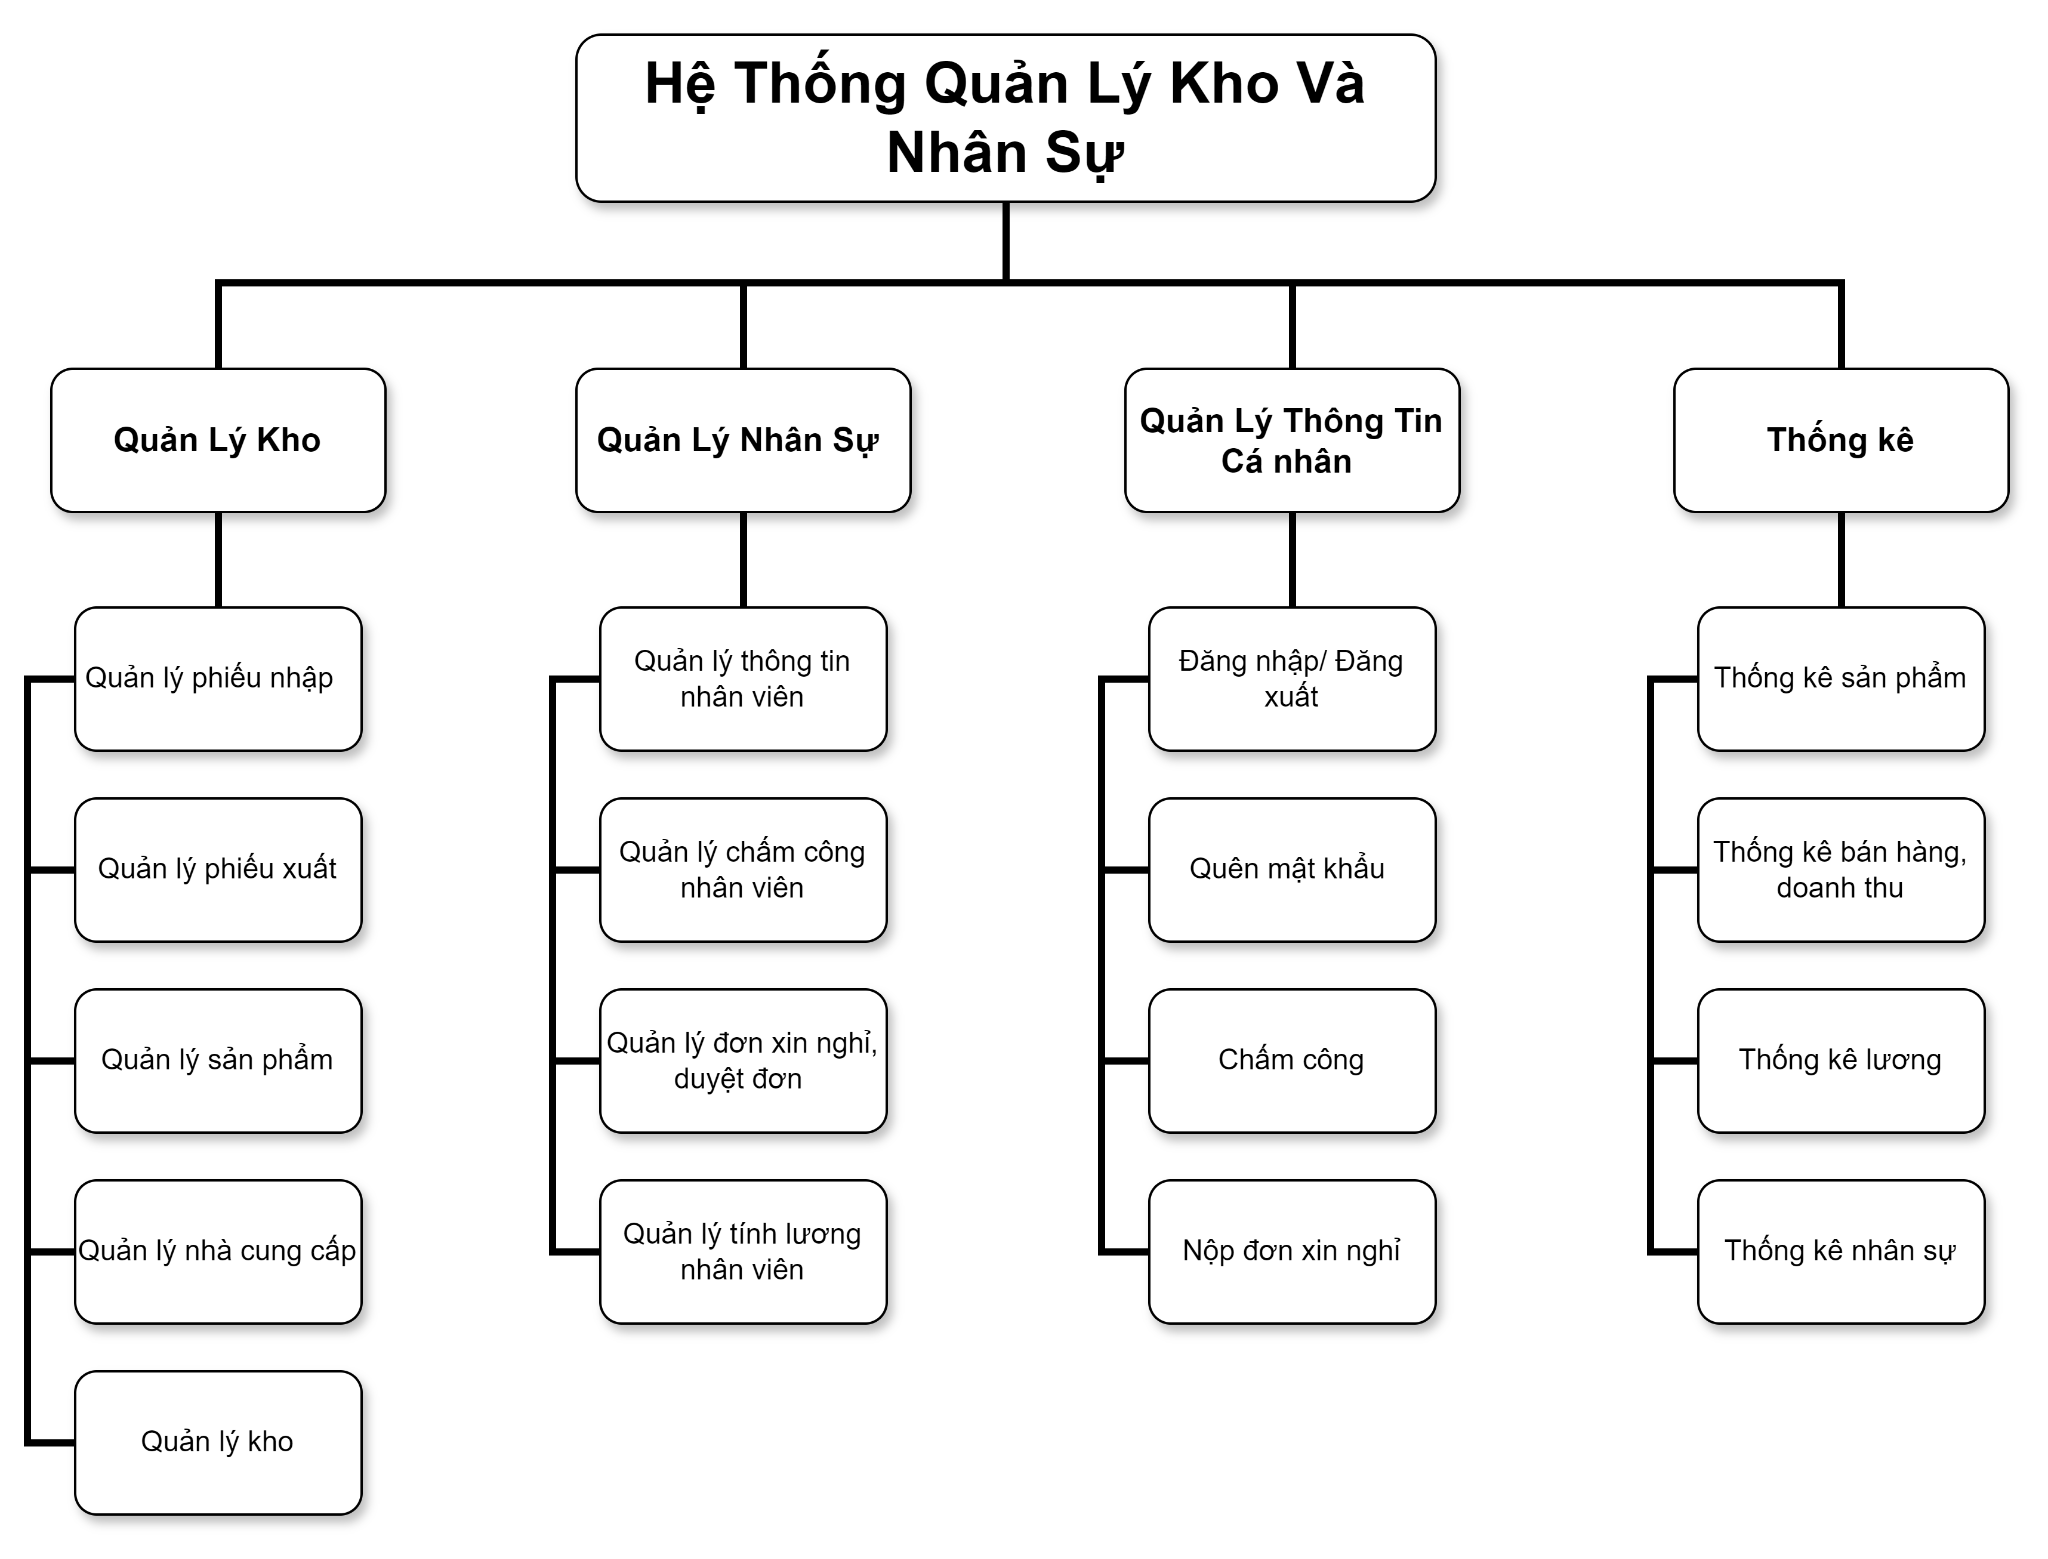
\includegraphics[width=1\linewidth]{image/Bao-cao-HTTTDN/BFD.png}
    \caption{Sơ đồ BFD.}
    \label{fig:image/Bao-cao-HTTTDN/BFD.png}
\end{figure}

\subsection{Sơ đồ ngữ cảnh}
\begin{figure}[H]
    \centering
    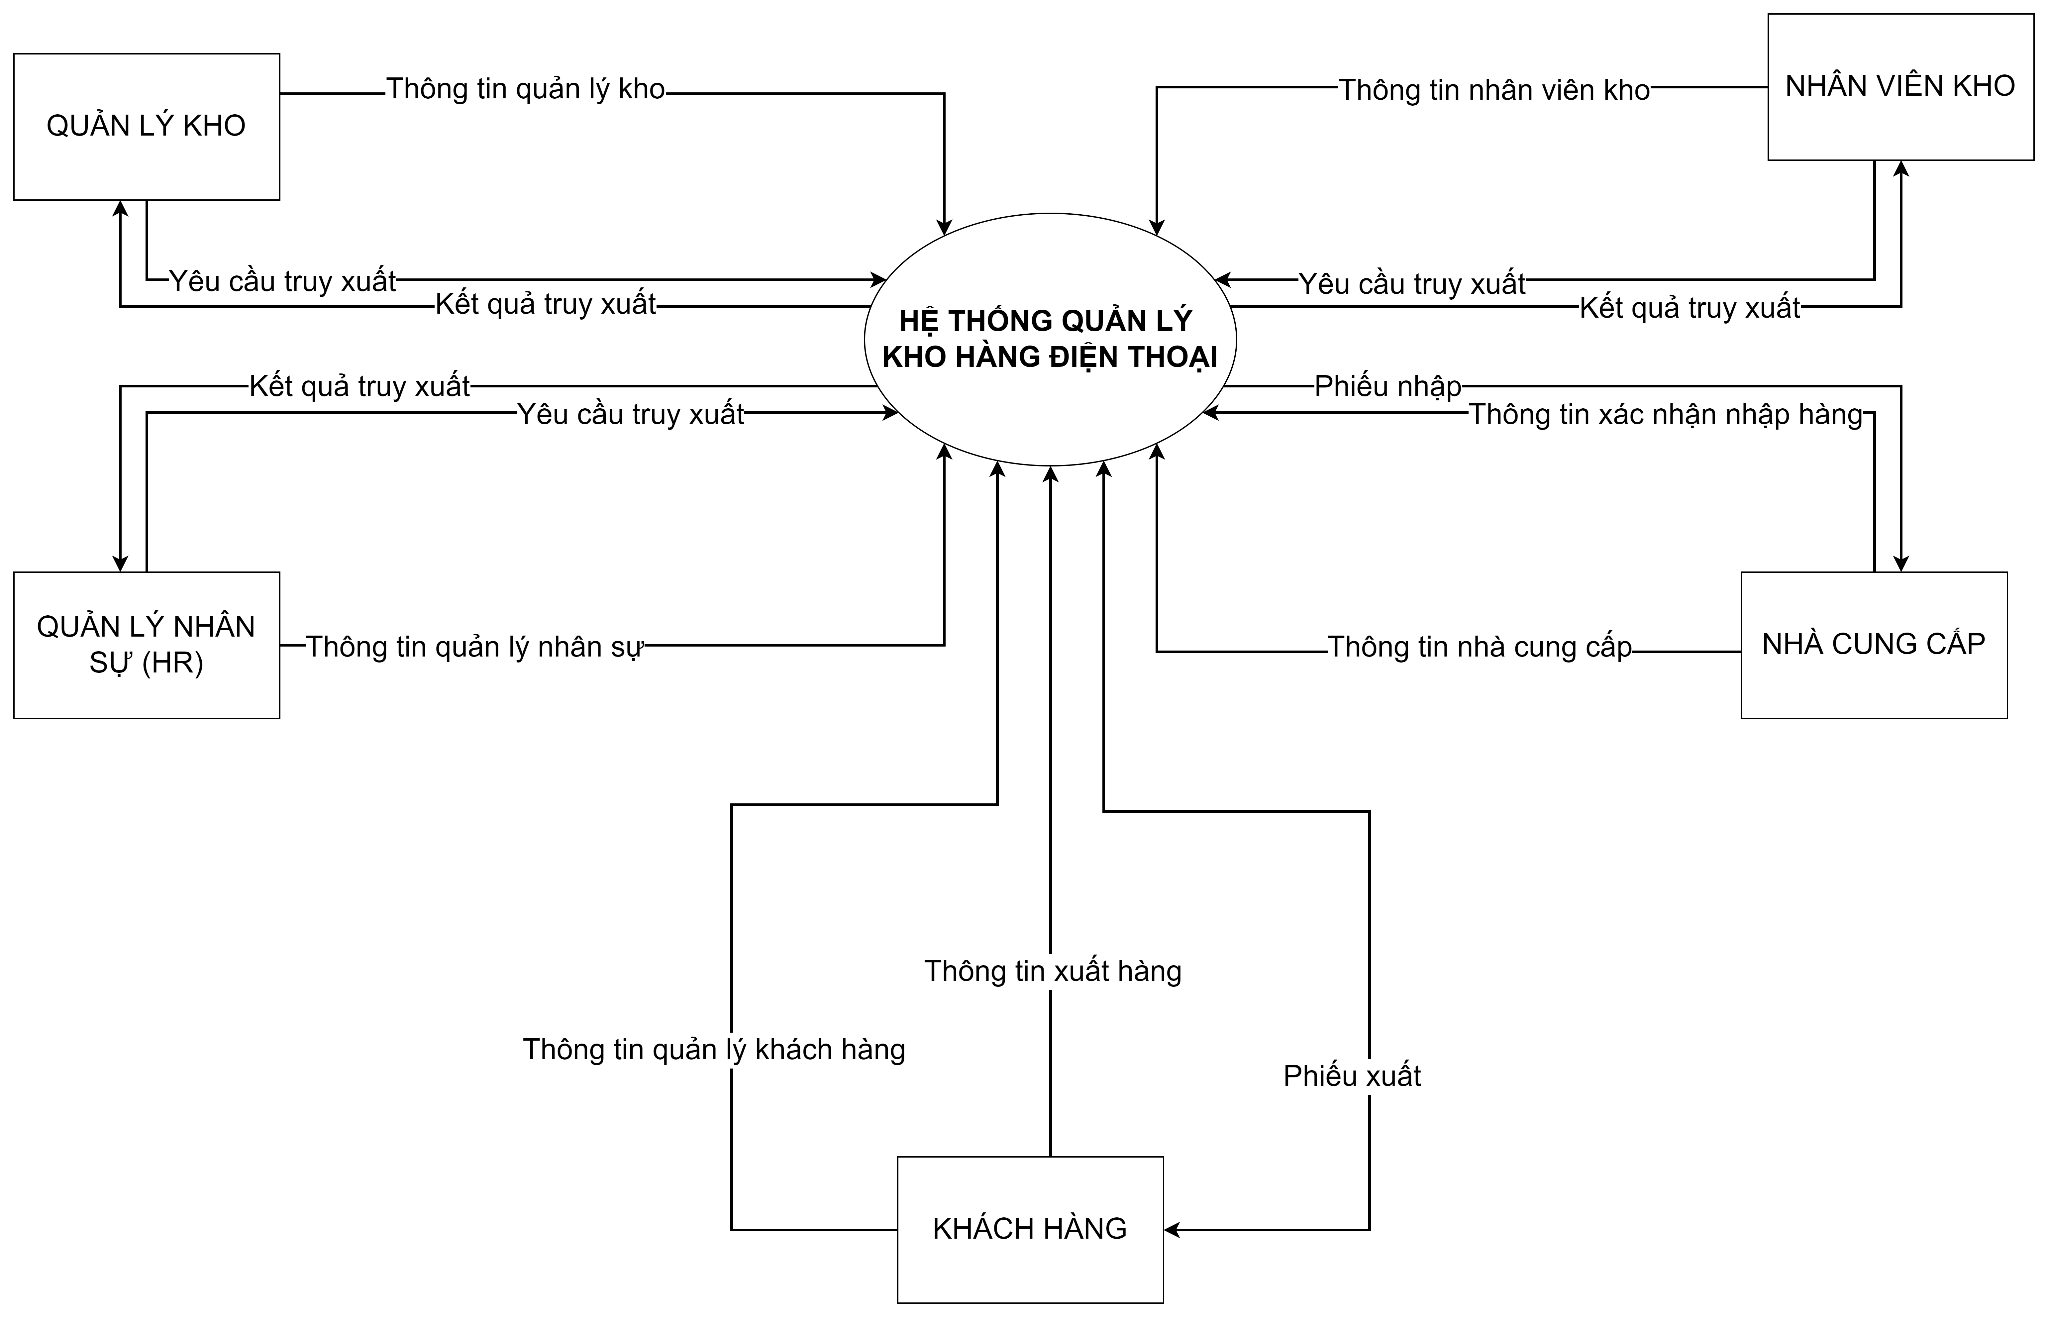
\includegraphics[width=1\linewidth]{image/Bao-cao-HTTTDN/SoDoNguCanh.png}
    \caption{Sơ đồ ngữ cảnh.}
    \label{fig:image/Bao-cao-HTTTDN/SoDoNguCanh}
\end{figure}
\subsection{Sơ đồ luồng dữ liệu mức đỉnh (DFD)}
\begin{figure}[H]
    \centering
    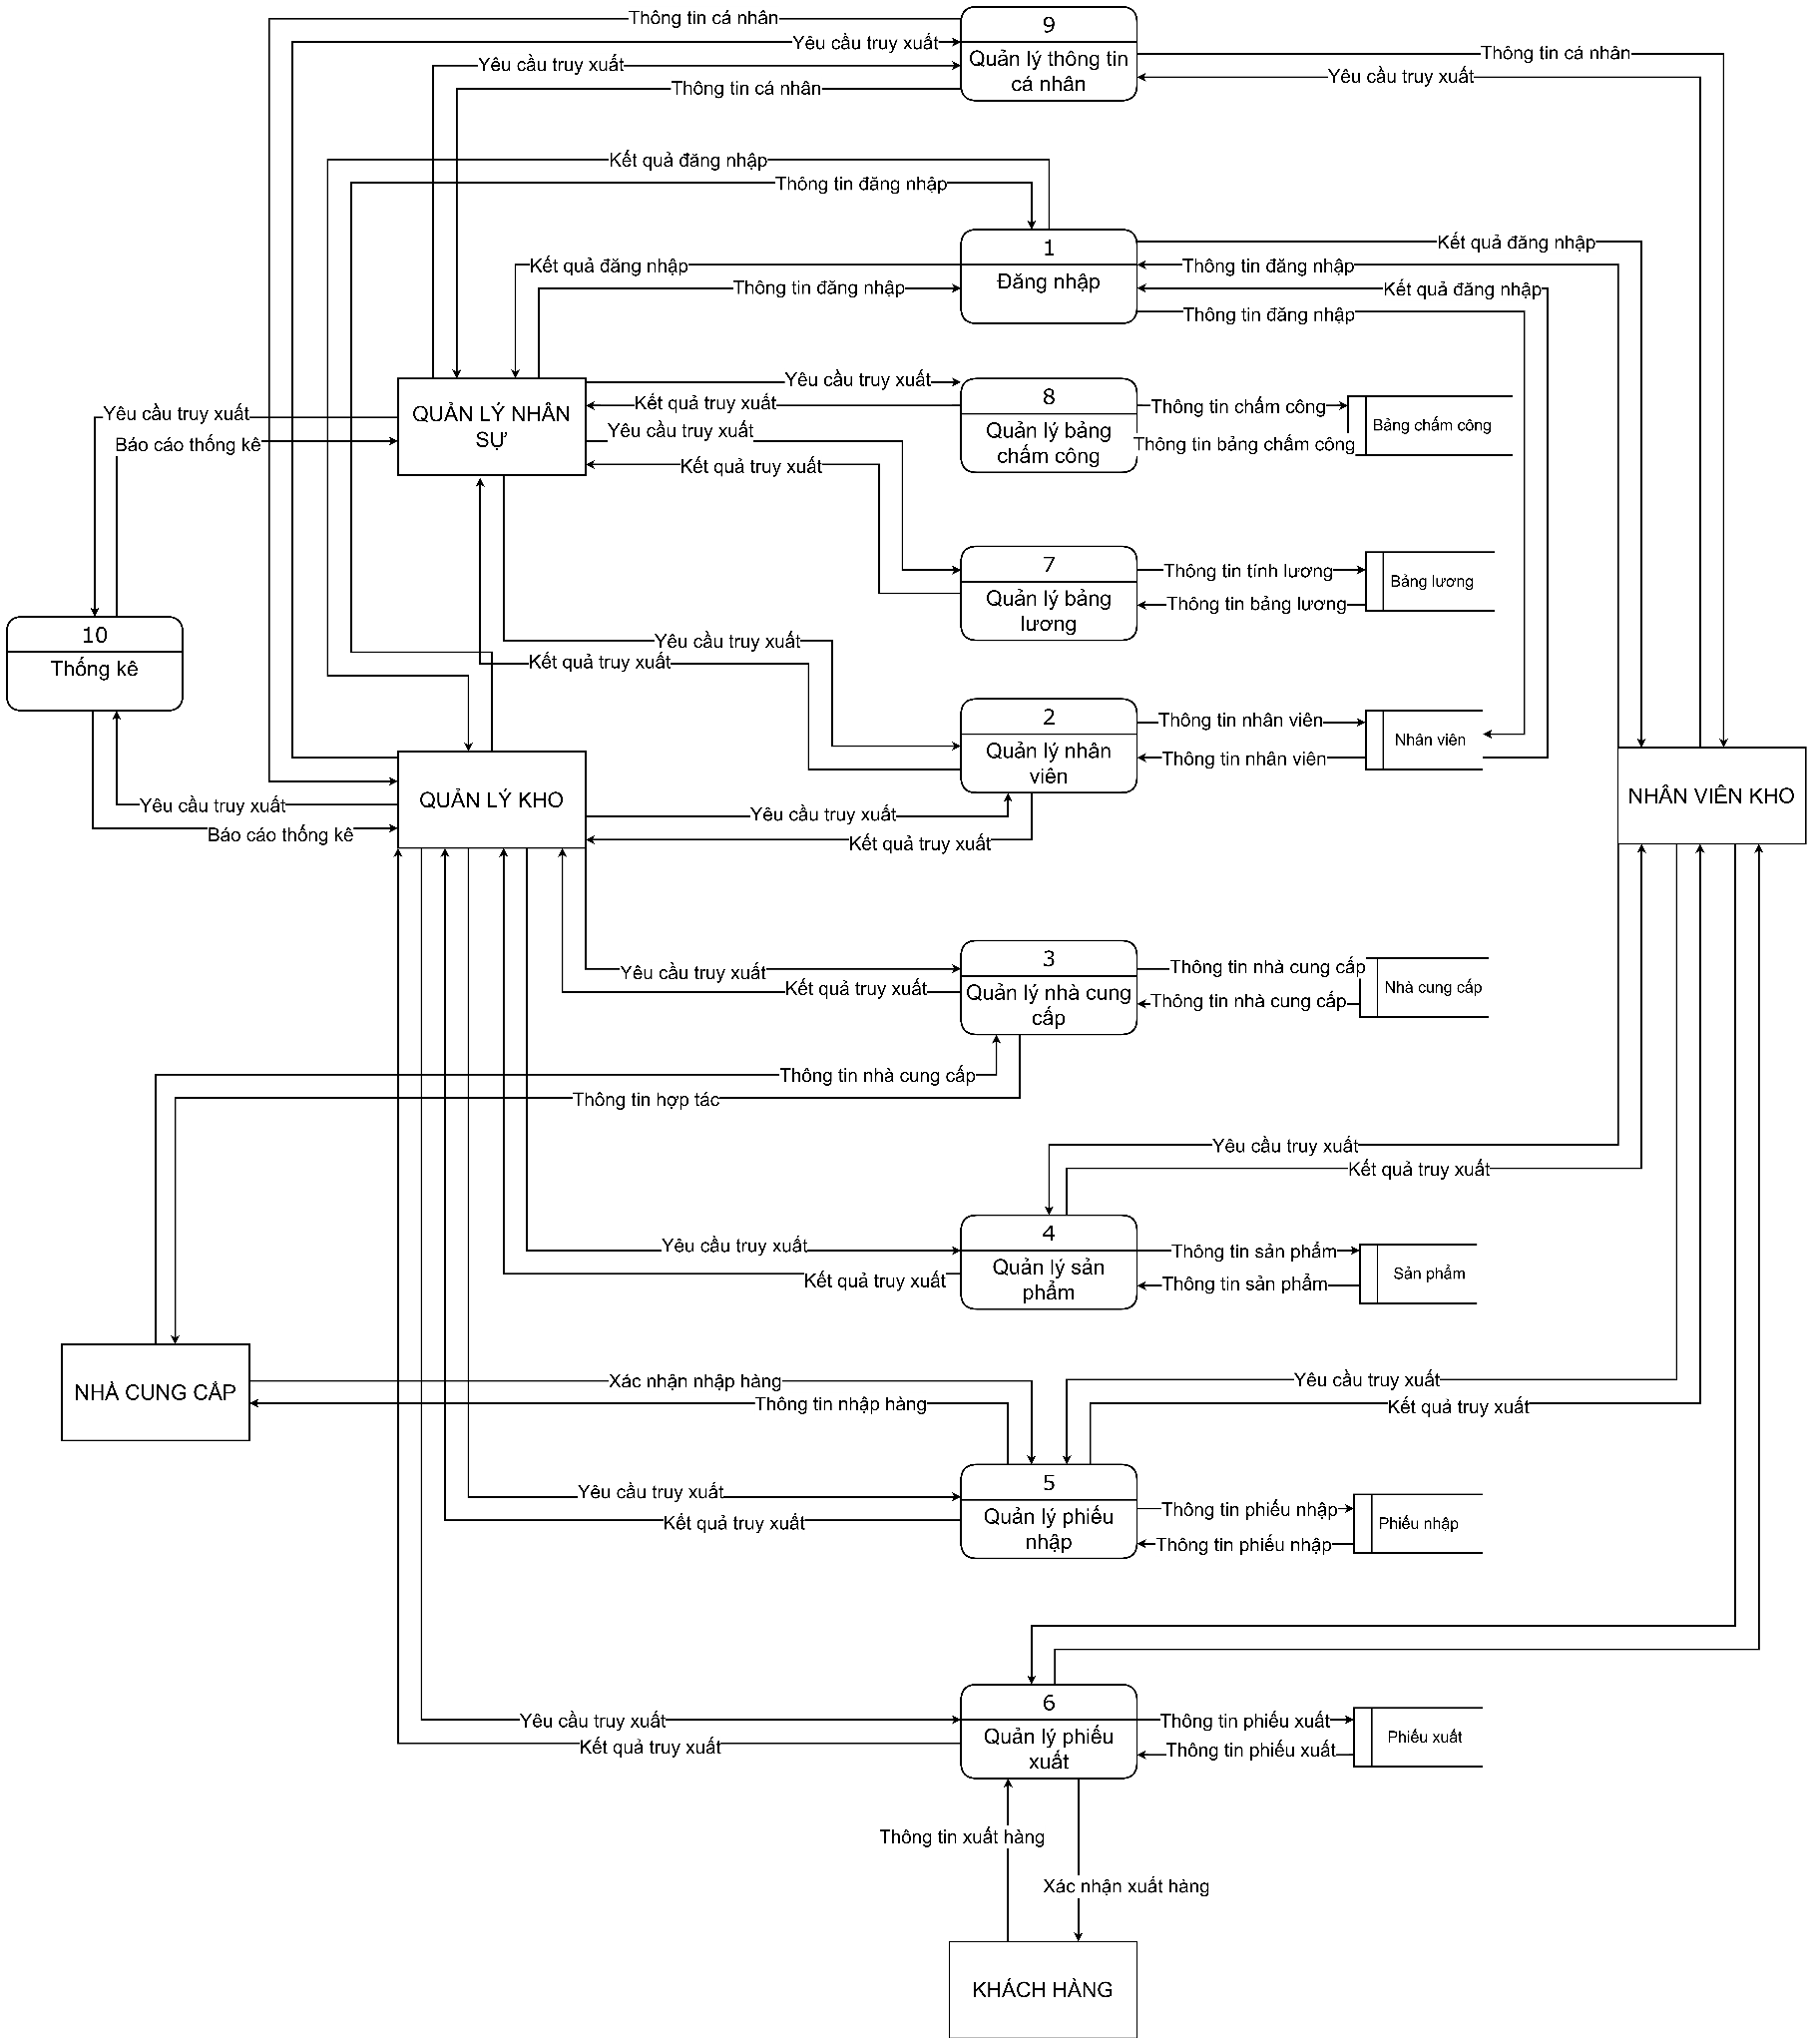
\includegraphics[width=1\linewidth]{image/Bao-cao-HTTTDN/DFD_MucDinh.png}
    \caption{Sơ đồ DFD.}
    \label{fig:image/Bao-cao-HTTTDN/DFD_MucDinh}
\end{figure}
\subsection{Sơ đồ luồng dữ liệu mức dưới đỉnh}
\begin{figure}[H]
    \centering
    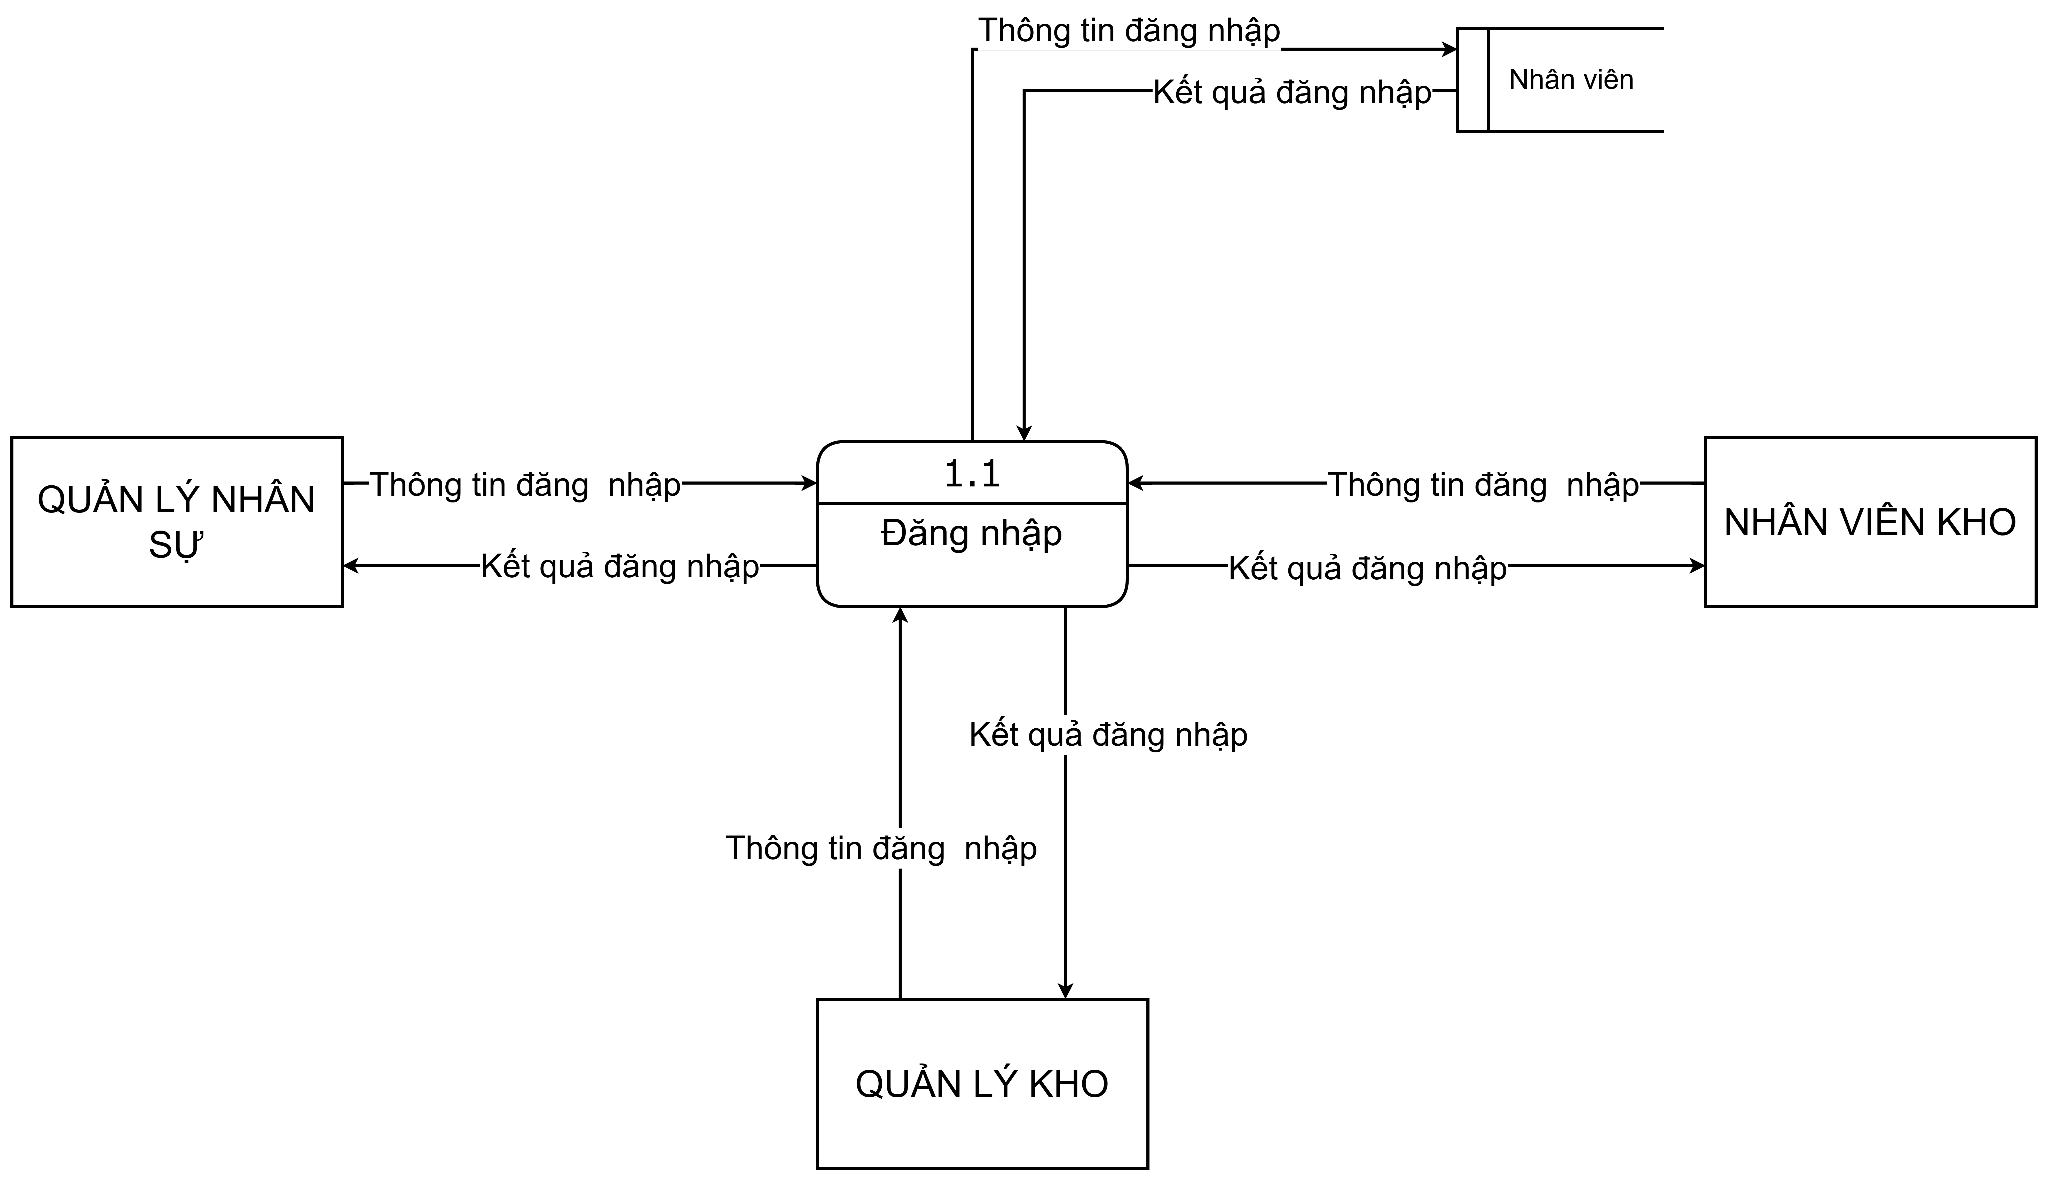
\includegraphics[width=0.8\linewidth]{image/Bao-cao-HTTTDN/DFD_DangNhap.png}
    \caption{Sơ đồ DFD đăng nhập.}
    \label{fig:image/Bao-cao-HTTTDN/DFD_DangNhap}
\end{figure}
\begin{figure}[H]
    \centering
    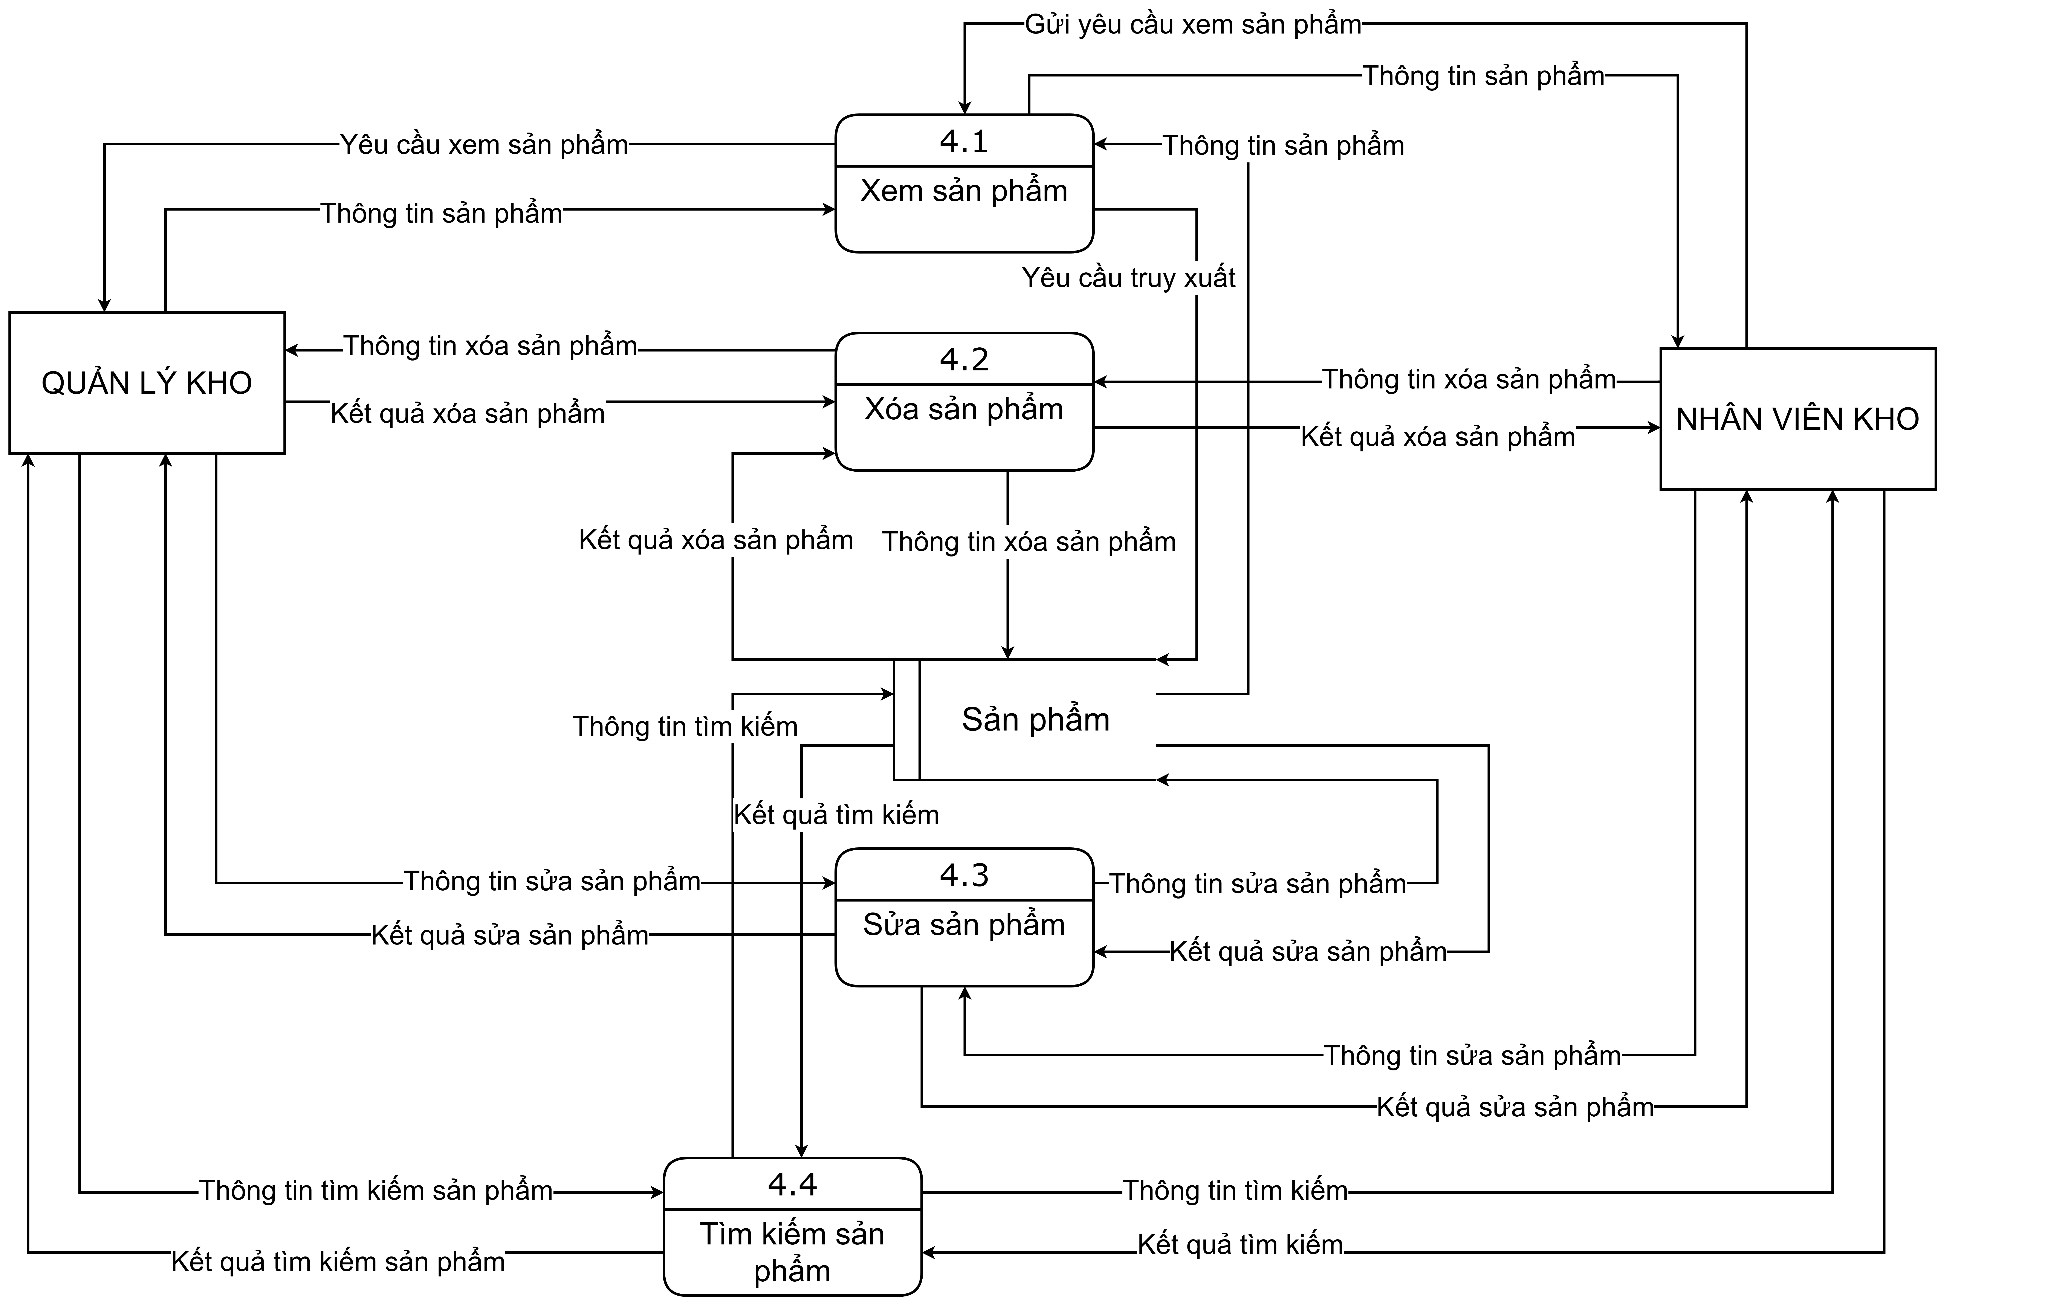
\includegraphics[width=0.8\linewidth]{image/Bao-cao-HTTTDN/DFD_SanPham.png}
    \caption{Sơ đồ DFD quản lý sản phẩm.}
    \label{fig:image/Bao-cao-HTTTDN/DFD_SanPham}
\end{figure}
\begin{figure}[H]
    \centering
    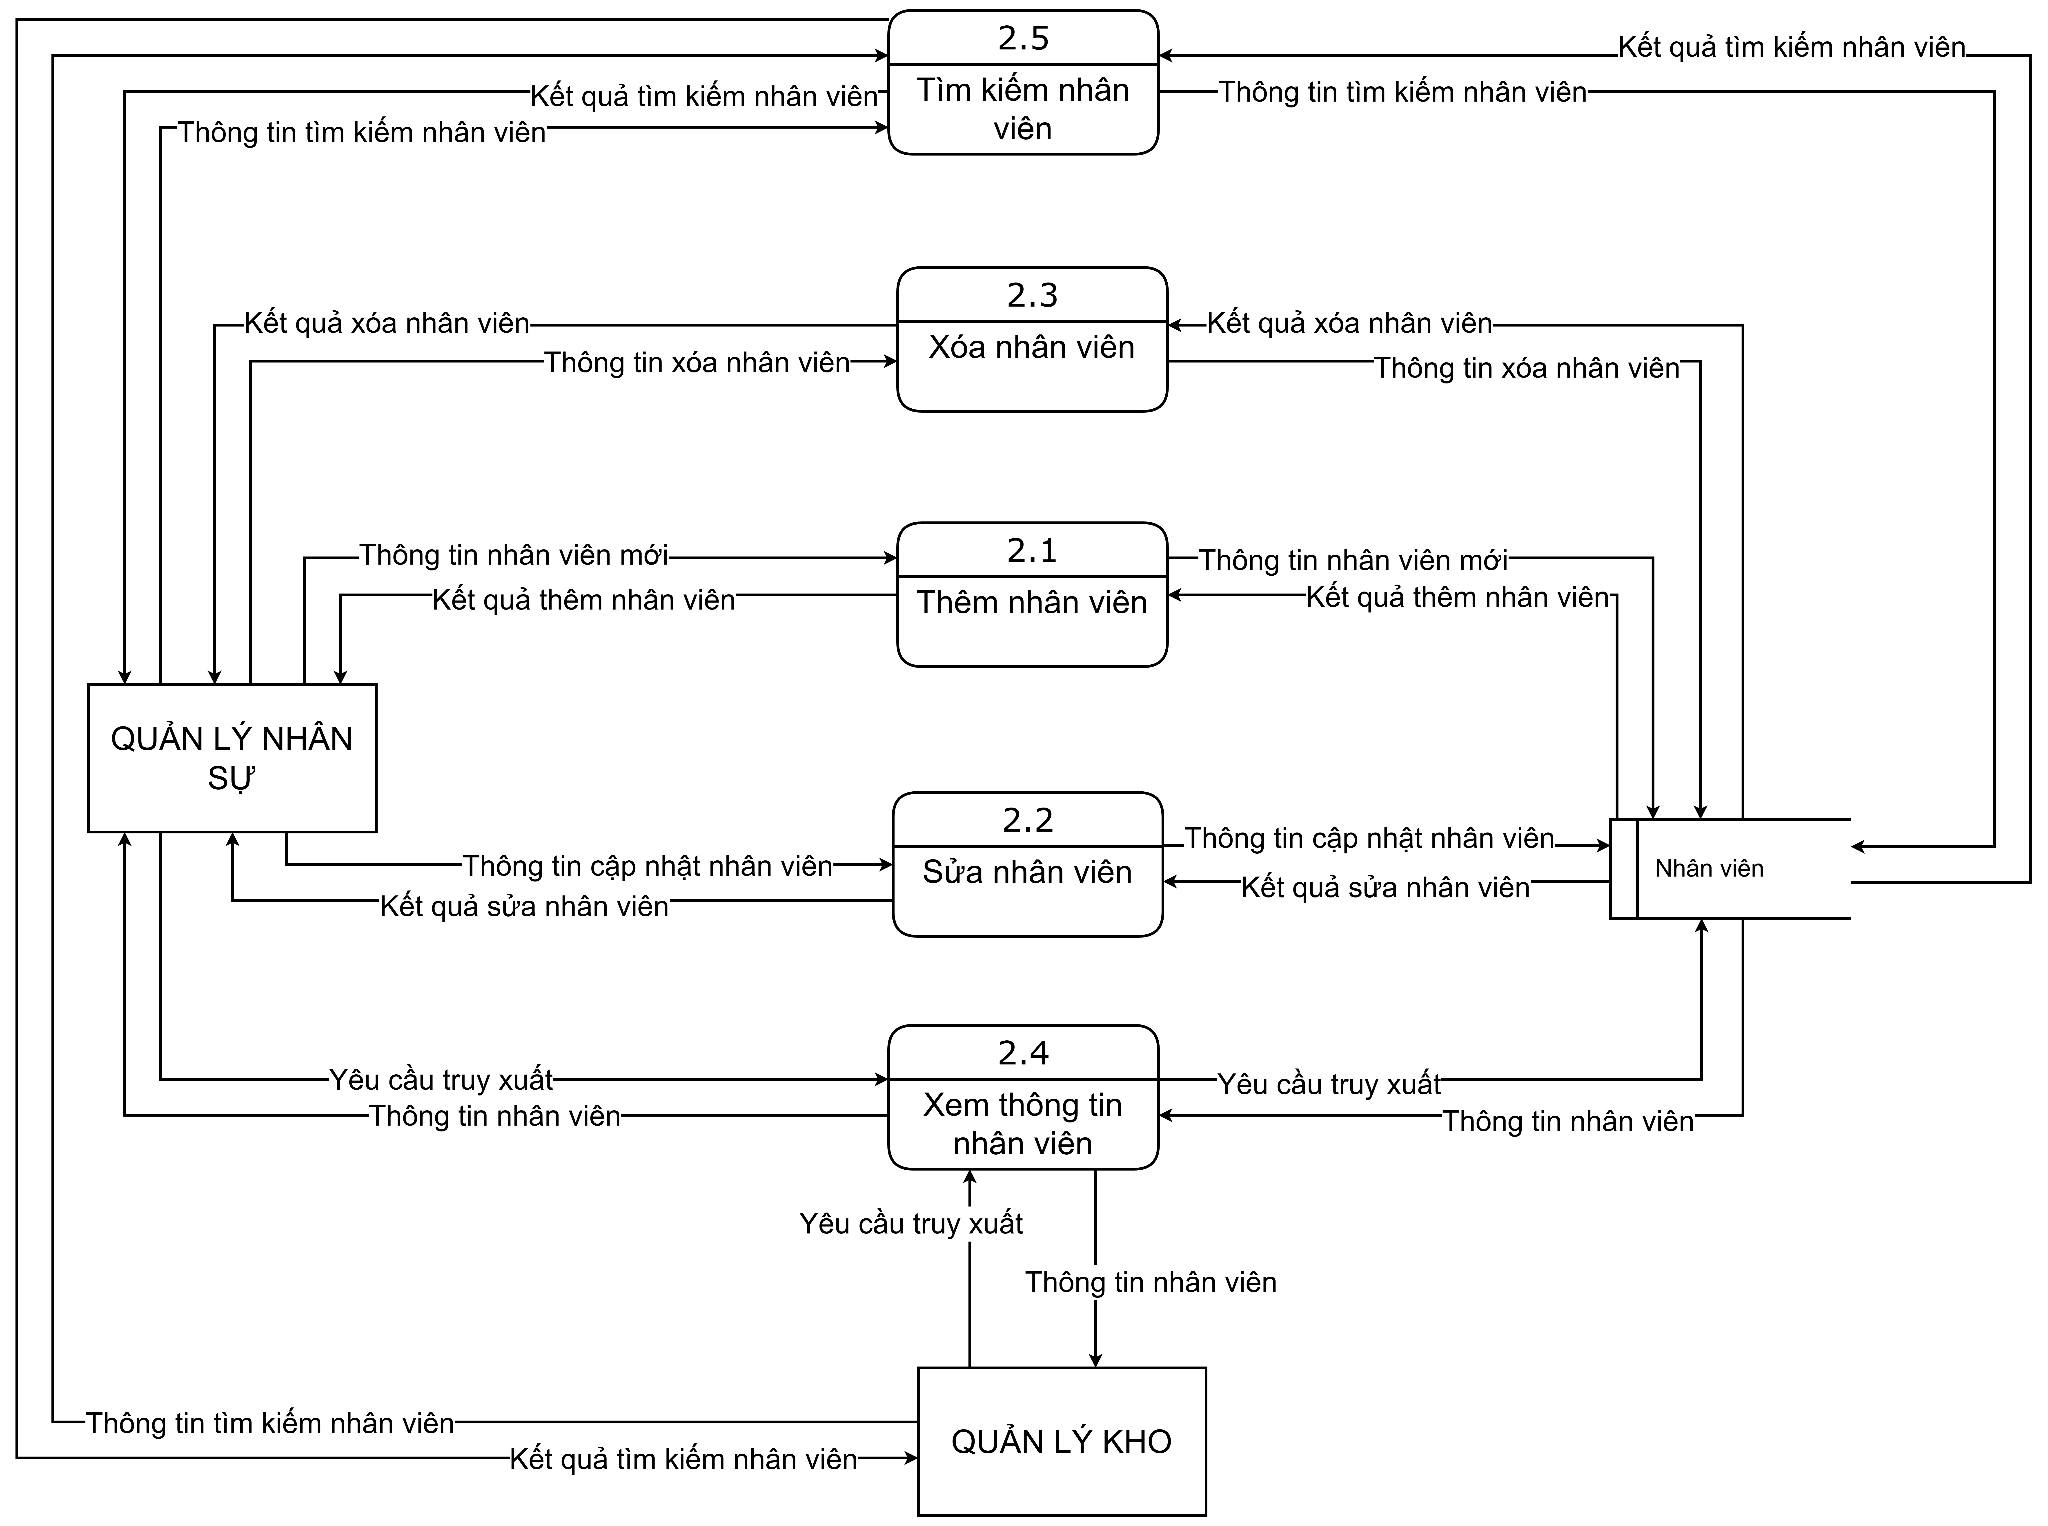
\includegraphics[width=0.8\linewidth]{image/Bao-cao-HTTTDN/DFD_NhanVien.png}
    \caption{Sơ đồ DFD quản lý nhân viên.}
    \label{fig:image/Bao-cao-HTTTDN/DFD_NhanVien}
\end{figure}
\begin{figure}[H]
    \centering
    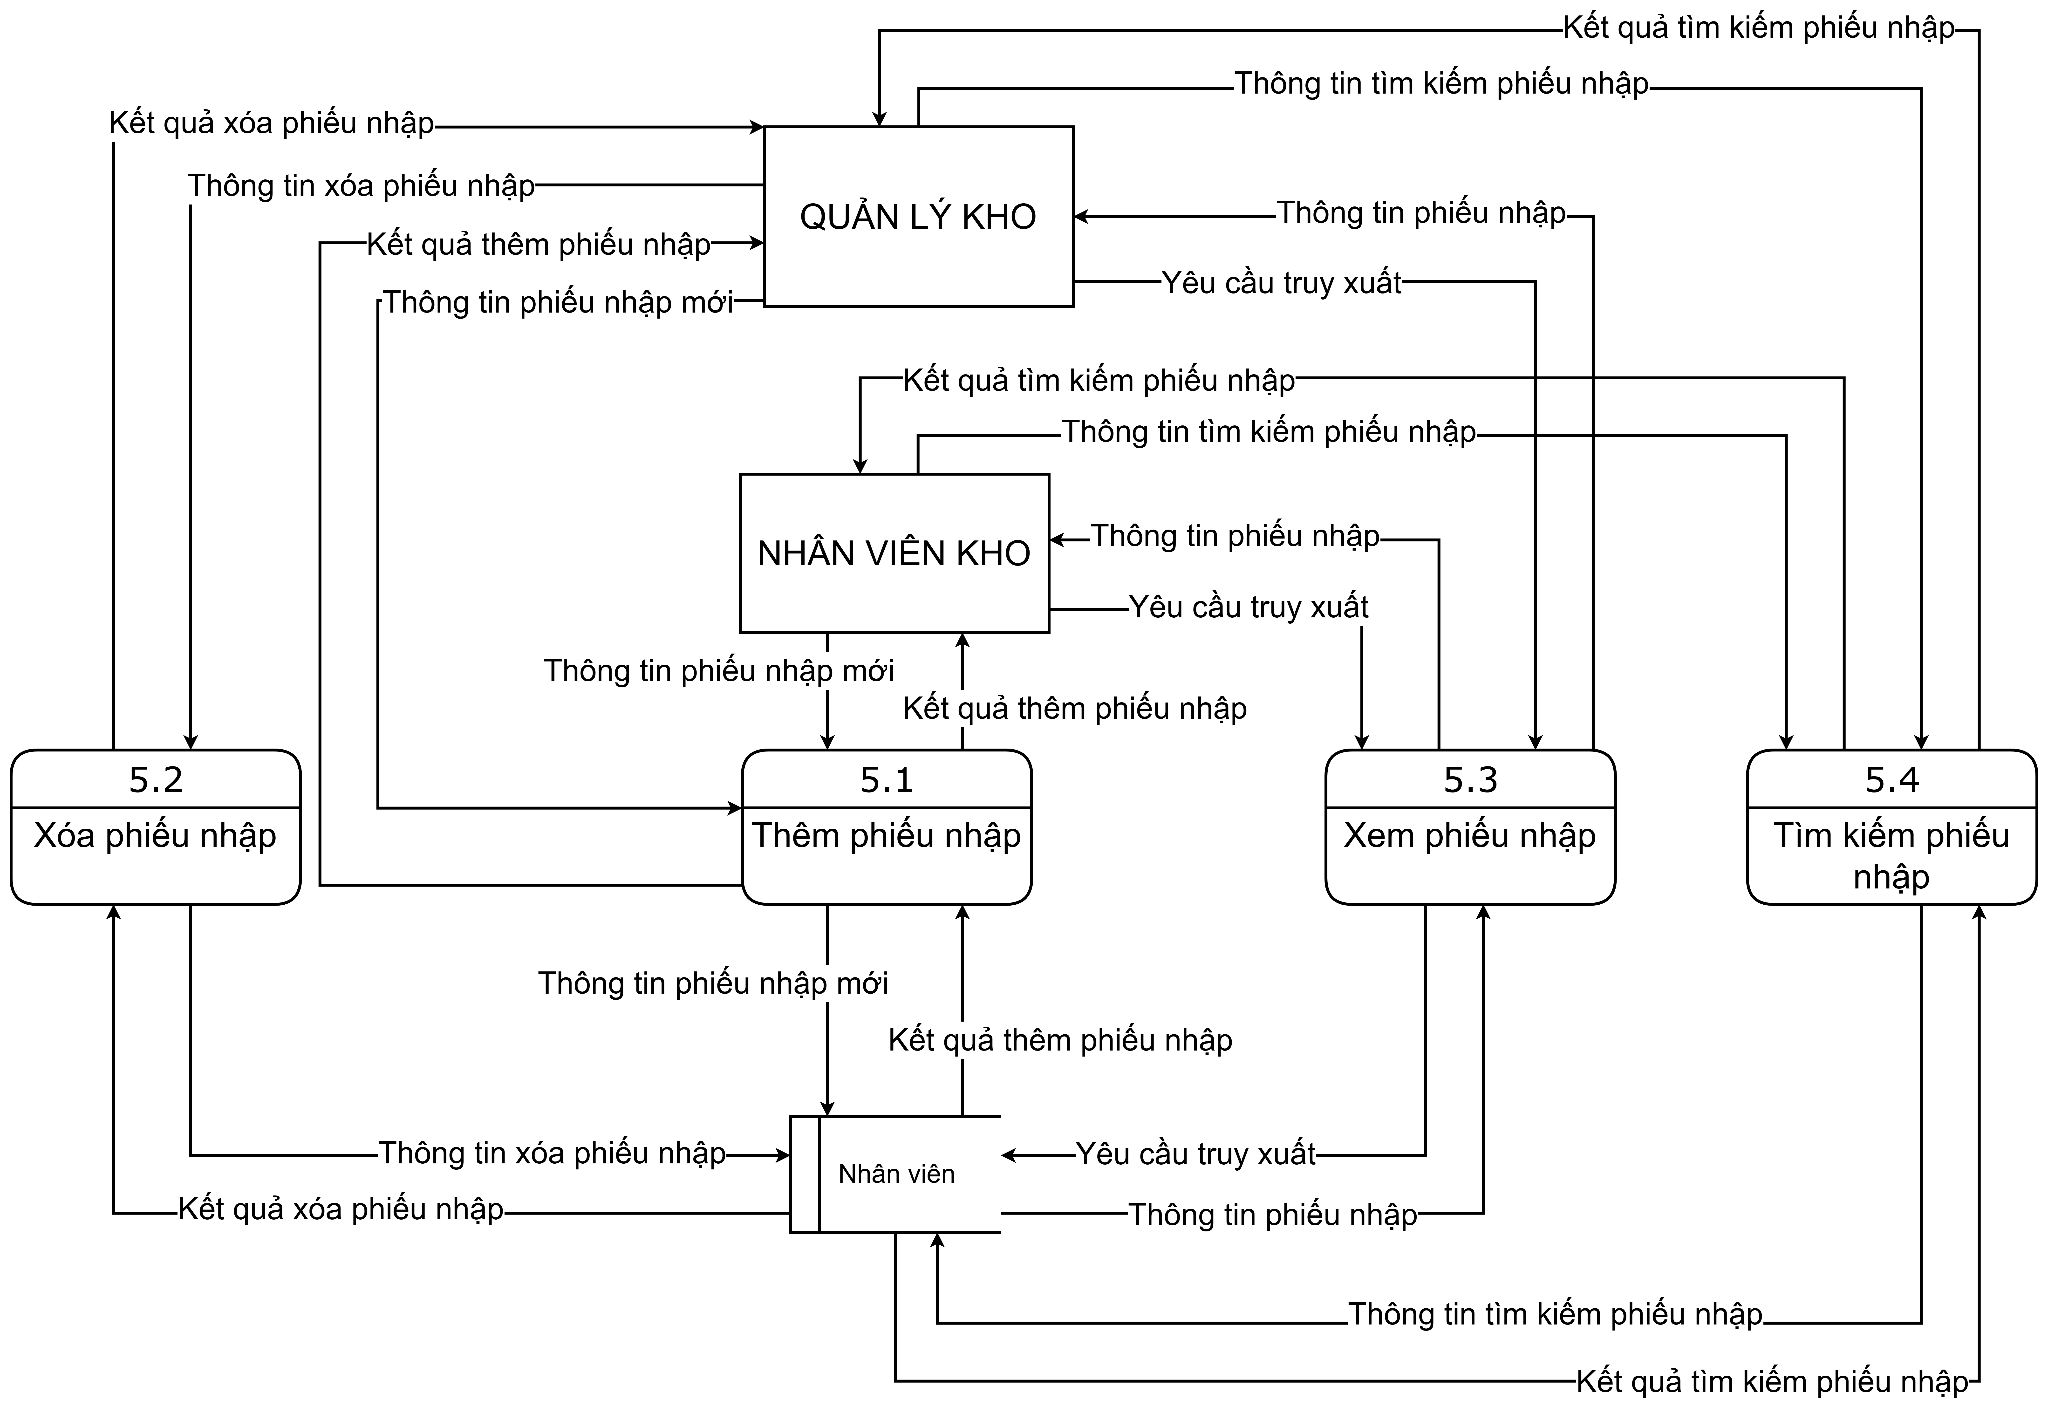
\includegraphics[width=0.8\linewidth]{image/Bao-cao-HTTTDN/DFD_PhieuNhap.png}
    \caption{Sơ đồ DFD quản lý phiếu nhập.}
    \label{fig:image/Bao-cao-HTTTDN/DFD_PhieuNhap}
\end{figure}
\begin{figure}[H]
    \centering
    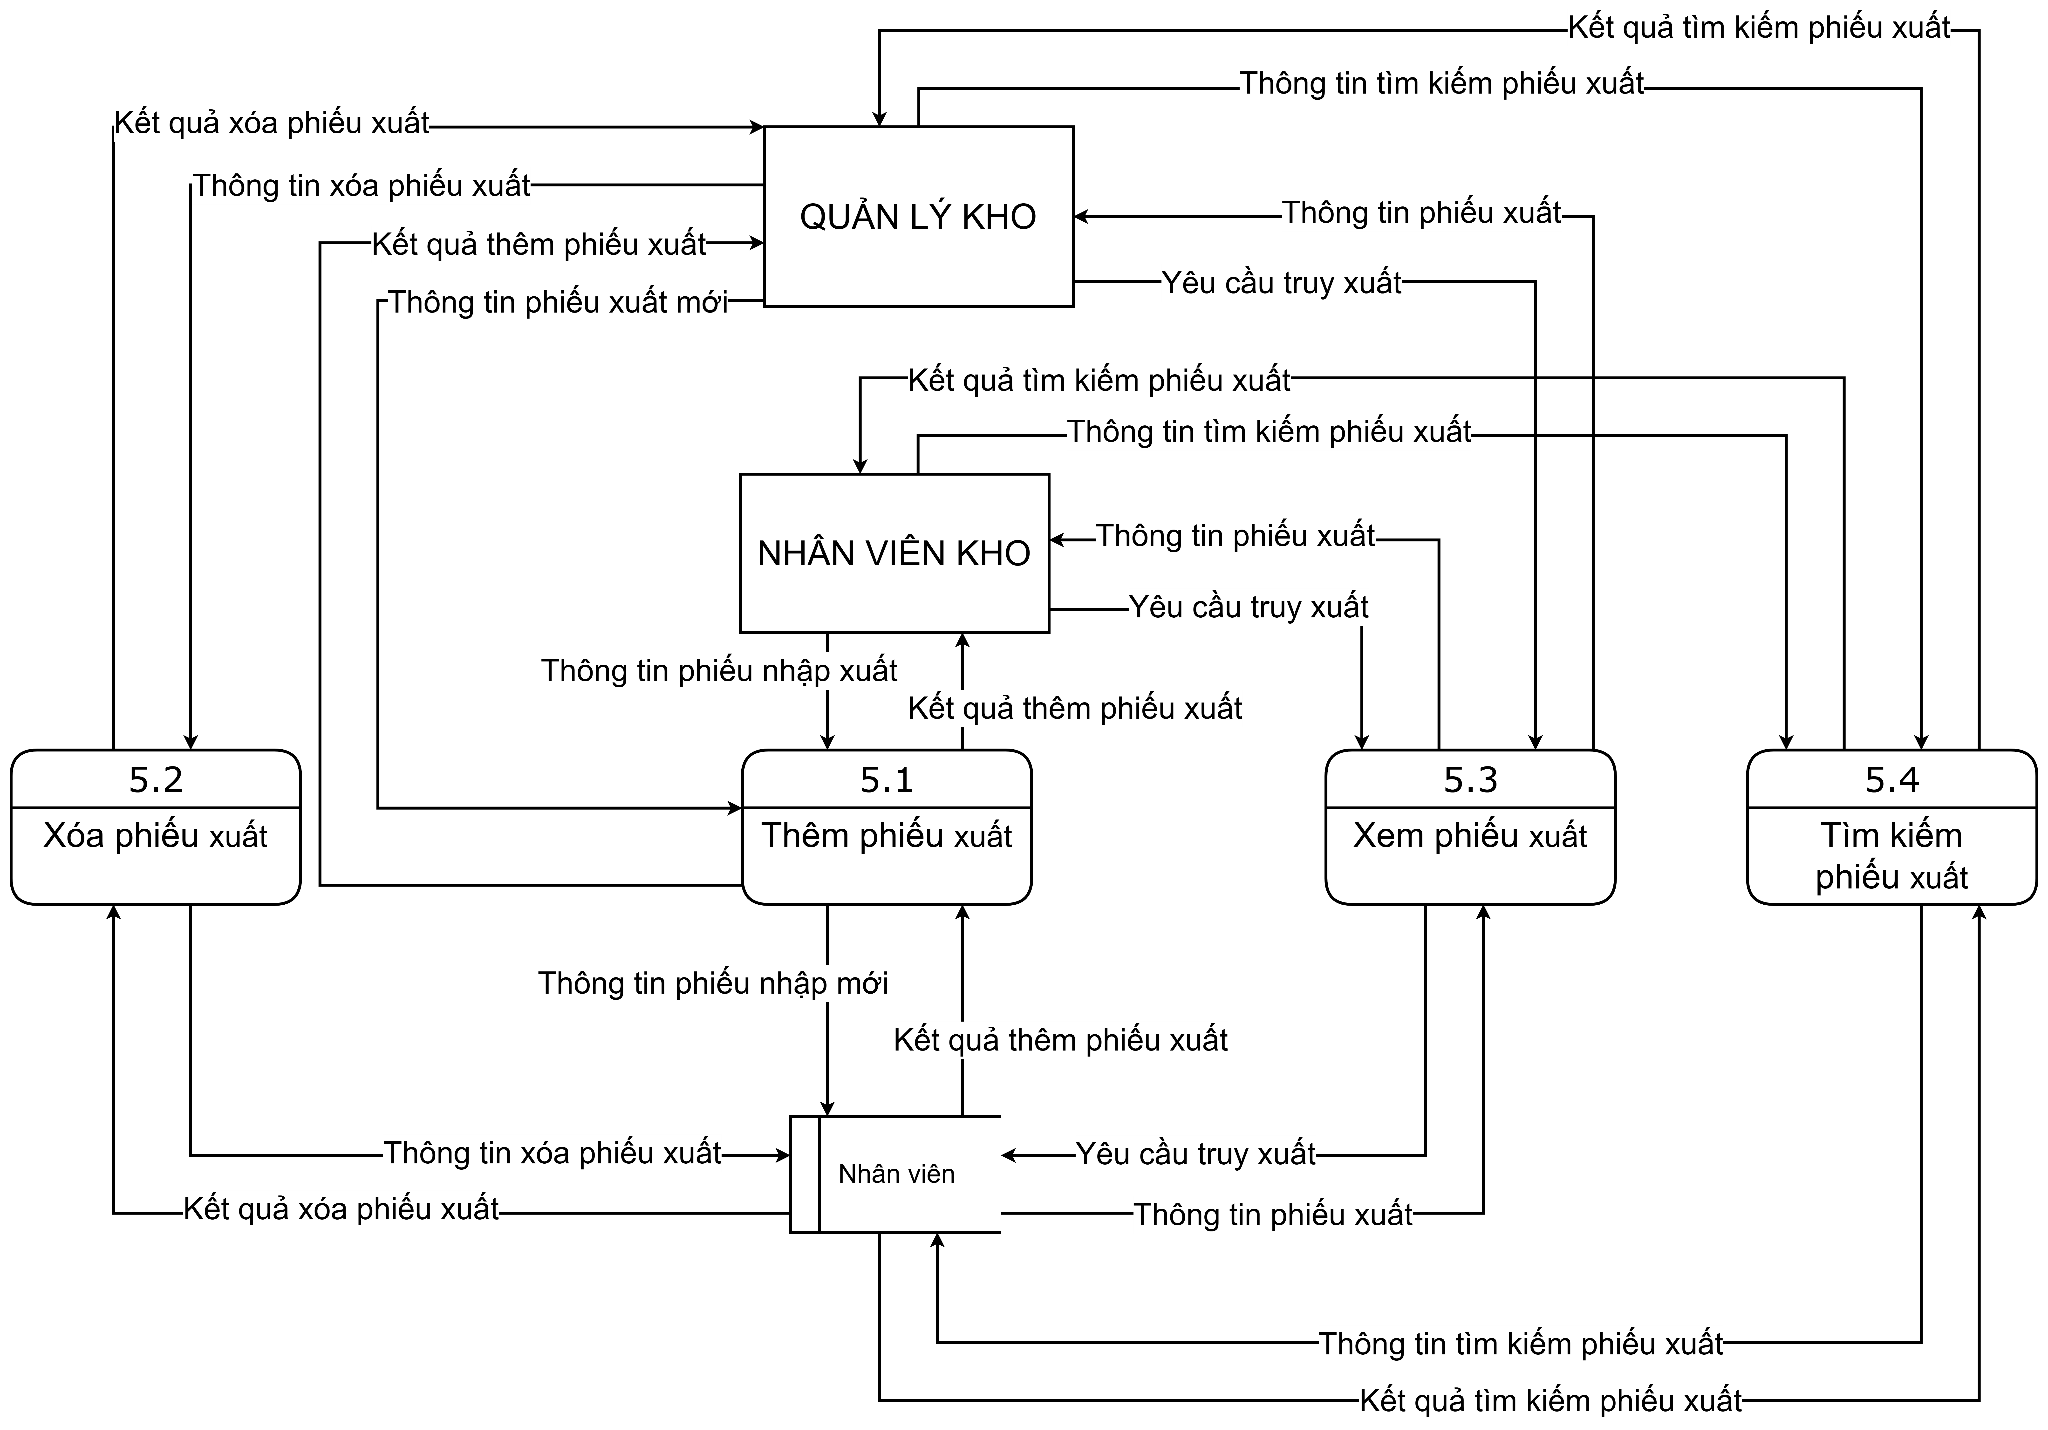
\includegraphics[width=0.8\linewidth]{image/Bao-cao-HTTTDN/DFD_PhieuXuat.png}
    \caption{Sơ đồ DFD quản lý phiếu xuất.}
    \label{fig:image/Bao-cao-HTTTDN/DFD_PhieuXuat}
\end{figure}
\begin{figure}[H]
    \centering
    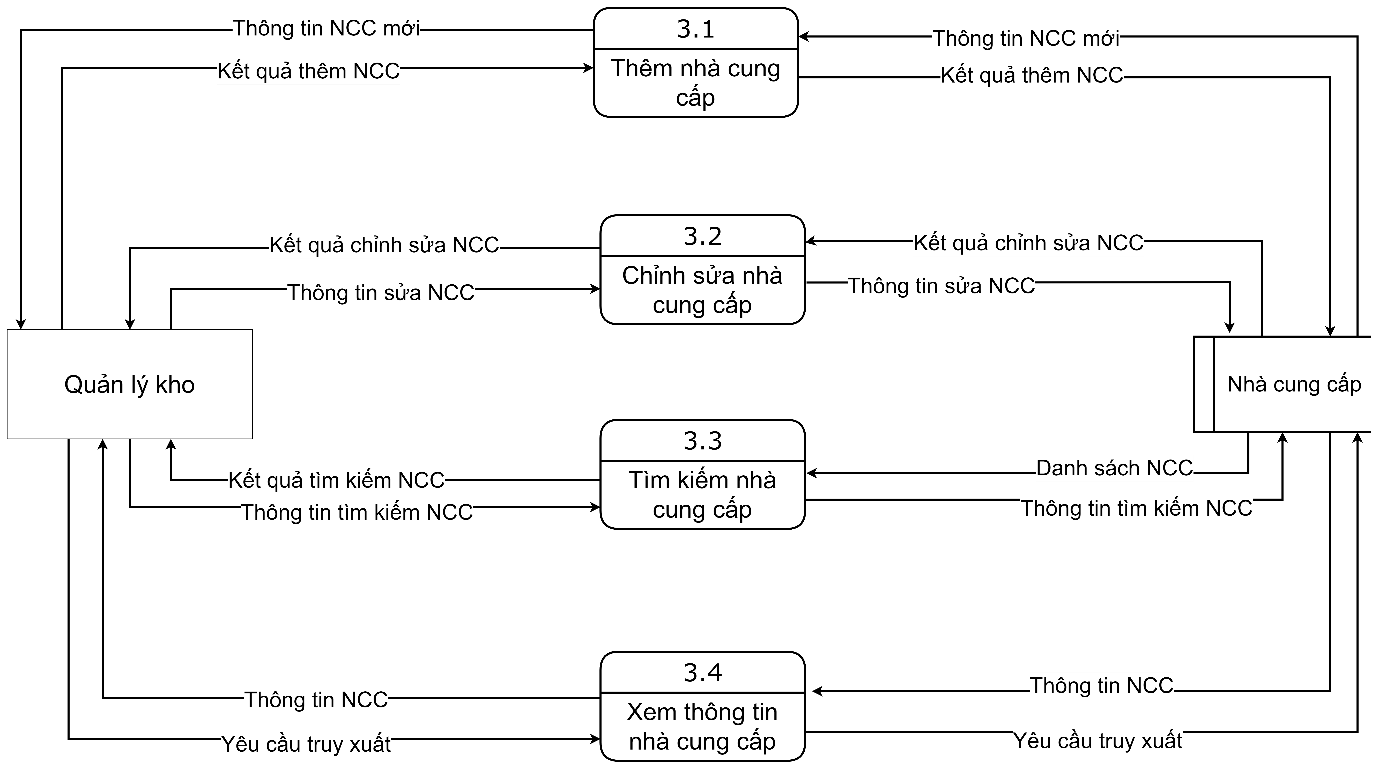
\includegraphics[width=0.8\linewidth]{image/Bao-cao-HTTTDN/DFD_NhaCungCap.png}
    \caption{Sơ đồ DFD quản lý nhà cung cấp.}
    \label{fig:image/Bao-cao-HTTTDN/DFD_NhaCungCap}
\end{figure}
\begin{figure}[H]
    \centering
    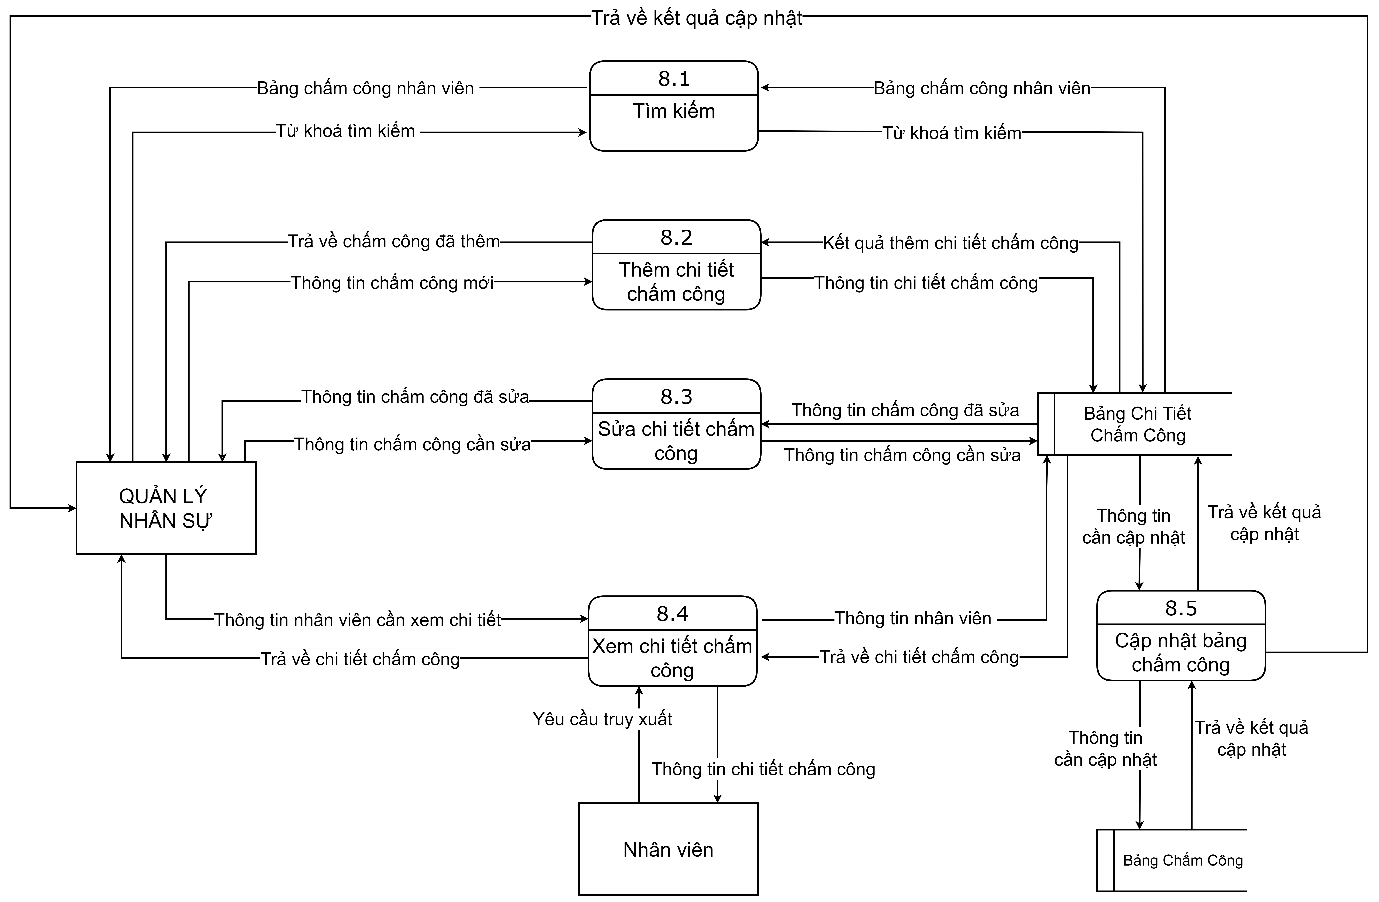
\includegraphics[width=0.7\linewidth]{image/Bao-cao-HTTTDN/DFD_ChamCong.png}
    \caption{Sơ đồ DFD quản lý bảng chấm công.}
    \label{fig:image/Bao-cao-HTTTDN/DFD_ChamCong}
\end{figure}
\begin{figure}[H]
    \centering
    \includegraphics[width=0.8\linewidth]{image/Bao-cao-HTTTDN/DFD_BangLuong.png}
    \caption{Sơ đồ DFD quản lý bảng lương.}
    \label{fig:image/Bao-cao-HTTTDN/DFD_BangLuong}
\end{figure}
\begin{figure}[H]
    \centering
    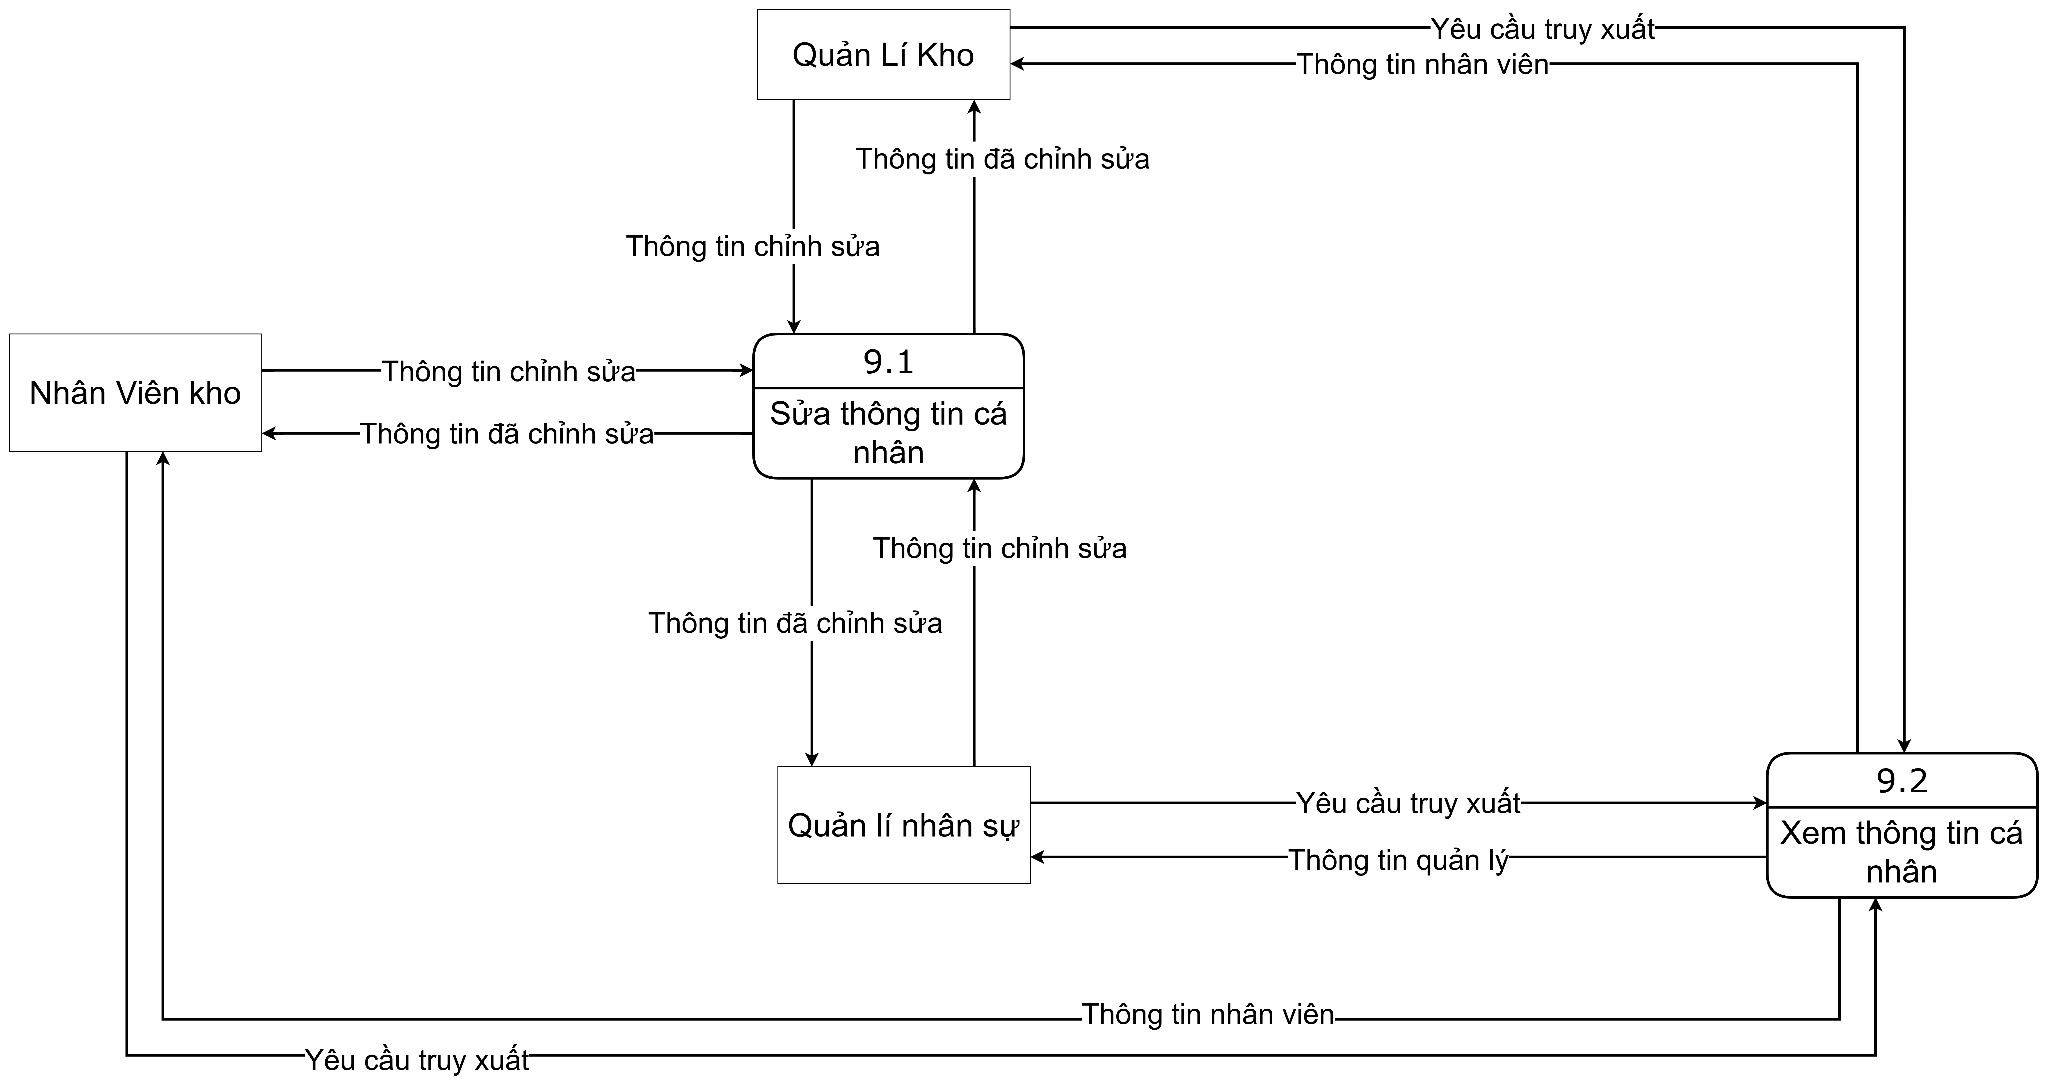
\includegraphics[width=0.8\linewidth]{image/Bao-cao-HTTTDN/DFD_ThongTinCN.png}
    \caption{Sơ đồ DFD quản lý thông tin cá nhân.}
    \label{fig:image/Bao-cao-HTTTDN/DFD_ThongTinCN}
\end{figure}
\begin{figure}[H]
    \centering
    \includegraphics[width=0.8\linewidth]{image/Bao-cao-HTTTDN/DFD_ThongKe.png}
    \caption{Sơ đồ DFD thống kê.}
    \label{fig:image/Bao-cao-HTTTDN/DFD_ThongKe}
\end{figure}
\section{Mô hình hóa cơ sở dữ liệu}
\subsection{Mô hình mối quan hệ thực thể (Entity Relationship \newline Diagram - ERD)}
\begin{figure}[H]
    \centering
    \includegraphics[width=1\linewidth]{image/Bao-cao-HTTTDN/ERD.png}
    \caption{Mô hình mối quan hệ thực thể - ERD.}
    \label{fig:image/Bao-cao-HTTTDN/ERD}
\end{figure}

\subsection{Sơ đồ quan hệ dữ liệu}
\begin{figure}[H]
    \centering
    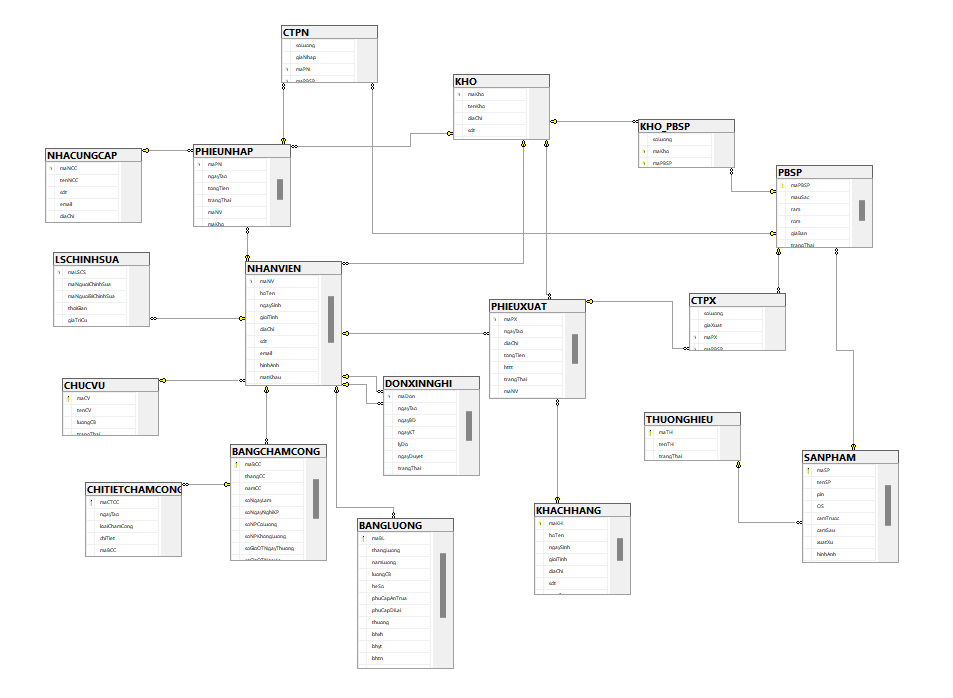
\includegraphics[width=0.9\linewidth]{image/Bao-cao-HTTTDN/so-do-quan-he-dl.png}
    \caption{Sơ đồ quan hệ dữ liệu.}
    \label{fig:image/Bao-cao-HTTTDN/so-do-quan-he-dl}
\end{figure}
\subsection{Mô tả các bảng dữ liệu}
\subsubsection{Bảng THƯƠNG HIỆU}
\noindent
\begin{center}
    \begin{tabular}{|>{\centering\arraybackslash}p{3cm}|
        >{\centering\arraybackslash}p{4cm}|
        >{\centering\arraybackslash}p{4cm}|
        >{\centering\arraybackslash}p{4cm}|}
        \hline
        \textbf{Thuộc tính}                                                                                                               &
        \textbf{Kiểu dữ liệu}                                                                                                                             &
        \textbf{Ý nghĩa}                                                                                                 &
        \textbf{Ràng buộc}                                                                                                         \\
        \hline
        maTH &  VARCHAR(50)  & Mã thương hiệu & PRIMARY KEY, NOT NULL \\
        \hline
        tenTH &  NVARCHAR(255)  & Tên thương hiệu & NOT NULL \\                                                                                                                          
        \hline
        trangThai &  VARCHAR(10)  & Trạng thái hoạt~động & CHECK(‘on’, ‘off’), NOT NULL \\
        \hline
    \end{tabular}
\end{center}
\newpage
\subsubsection{Bảng SẢN PHẨM}
\noindent
\begin{center}
    \begin{tabular}{|>{\centering\arraybackslash}p{3cm}|
        >{\centering\arraybackslash}p{4cm}|
        >{\centering\arraybackslash}p{4cm}|
        >{\centering\arraybackslash}p{4cm}|}
        \hline
        \textbf{Thuộc tính}                                                                                                               &
        \textbf{Kiểu dữ liệu}                                                                                                                             &
        \textbf{Ý nghĩa}                                                                                                 &
        \textbf{Ràng buộc}                                                                                                         \\
        \hline
        maSP &  VARCHAR(50)  & Mã sản phẩm & PRIMARY KEY, NOT NULL \\
        \hline
        tenSP &  NVARCHAR(255)  & Tên sản phẩm & NOT NULL \\
        \hline
        pin & NVARCHAR(50) & Dung lượng pin & NOT NULL \\                                                                                                                          
        \hline
        OS & NVARCHAR(50) & Hệ điều hành & NOT NULL \\                                                                                                                          
        \hline
        camTruoc & NVARCHAR(50) & Camera trước & NOT NULL \\                                                                                                                          
        \hline
        camSau & NVARCHAR(50) & Camera sau & NOT NULL \\                                                                                                                          
        \hline
        xuatXu & NVARCHAR(50) & Xuất xứ & NOT NULL \\                                                                                                                          
        \hline
        hinhAnh & NVARCHAR(50) & Hình ảnh (dạng BLOB) & NOT NULL \\                                                                                                                          
        \hline
        trangThai &  VARCHAR(10)  & Trạng thái sản~phẩm & CHECK(‘on’, ‘off’), NOT NULL \\
        \hline
        maTH & VARCHAR(50) & Mã thương hiệu & NOT NULL, FOREIGN KEY references THUONGHIEU \\                                                                                                                          
        \hline
    \end{tabular}
\end{center}
\subsubsection{Bảng PHIÊN BẢN SẢN PHẨM}
\noindent
\begin{center}
    \begin{longtable}{|>{\centering\arraybackslash}p{3cm}|
        >{\centering\arraybackslash}p{4cm}|
        >{\centering\arraybackslash}p{4cm}|
        >{\centering\arraybackslash}p{4cm}|}
        \hline
        \textbf{Thuộc tính}                                                                                                               &
        \textbf{Kiểu dữ liệu}                                                                                                                             &
        \textbf{Ý nghĩa}                                                                                                 &
        \textbf{Ràng buộc}                                                                                                         \\
        \hline
        maPBSP &  VARCHAR(50)  & Mã phiên bản sản phẩm & PRIMARY KEY, NOT NULL \\
        \hline
        mauSac &  NVARCHAR(50)  & Màu sắc & NOT NULL \\                                                                                                                          
        \hline
        ram & NVARCHAR(50) & Dung lượng RAM & NOT NULL \\                                                                                                                          
        \hline
        rom & NVARCHAR(50) & Dung lượng ROM & NOT NULL \\                                                                                                                          
        \hline
        giaBan & DECIMAL(18, 2) & Giá bán & NOT NULL \\                                                                                                                          
        \hline
        trangThai &  VARCHAR(10)  & Trạng thái phiên~bản & CHECK(‘on’, ‘off’), NOT NULL \\
        \hline
        maSP & VARCHAR(50) & Mã sản phẩm & NOT NULL, FOREIGN KEY references SANPHAM \\                                                                                                                          
        \hline
    \end{longtable}
\end{center}
\subsubsection{Bảng NHÀ CUNG CẤP}
\noindent
\begin{center}
    \begin{tabular}{|>{\centering\arraybackslash}p{3cm}|
        >{\centering\arraybackslash}p{4cm}|
        >{\centering\arraybackslash}p{4cm}|
        >{\centering\arraybackslash}p{4cm}|}
        \hline
        \textbf{Thuộc tính}                                                                                                               &
        \textbf{Kiểu dữ liệu}                                                                                                                             &
        \textbf{Ý nghĩa}                                                                                                 &
        \textbf{Ràng buộc}                                                                                                         \\
        \hline
        maNCC &  VARCHAR(50)  & Mã nhà cung cấp & PRIMARY KEY, NOT NULL \\
        \hline
        tenNCC &  NVARCHAR(255)  & Tên nhà cung cấp & NOT NULL \\                                                                                                                          
        \hline
        sdt & NVARCHAR(20) & Số điện thoại & NOT NULL \\                                                                                                                          
        \hline
        email & NVARCHAR(255) & Email &  \\                                                                                                                          
        \hline
        diaChi & NVARCHAR(255) & Địa chỉ & \\                                                                                                                          
        \hline
        trangThai &  VARCHAR(10)  & Trạng thái hoạt~động & CHECK(‘on’, ‘off’), NOT NULL \\
        \hline
    \end{tabular}
\end{center}
\subsubsection{Bảng CHỨC VỤ}
\noindent
\begin{center}
    \begin{tabular}{|>{\centering\arraybackslash}p{3cm}|
        >{\centering\arraybackslash}p{4cm}|
        >{\centering\arraybackslash}p{4cm}|
        >{\centering\arraybackslash}p{4cm}|}
        \hline
        \textbf{Thuộc tính}                                                                                                               &
        \textbf{Kiểu dữ liệu}                                                                                                                             &
        \textbf{Ý nghĩa}                                                                                                 &
        \textbf{Ràng buộc}                                                                                                         \\
        \hline
        maCV &  VARCHAR(50)  & Mã chức vụ & PRIMARY KEY, NOT NULL \\
        \hline
        tenCV &  NVARCHAR(255)  & Tên chức vụ & NOT NULL \\                                                                                                                          
        \hline
        luongCB & FLOAT & Lương cơ bản & NOT NULL \\                                                                                                                          
        \hline
        trangThai &  VARCHAR(50)  & Trạng thái hoạt~động & CHECK(‘on’, ‘off’), NOT NULL \\
        \hline
    \end{tabular}
\end{center}
\subsubsection{Bảng KHO}
\noindent
\begin{center}
    \begin{tabular}{|>{\centering\arraybackslash}p{3cm}|
        >{\centering\arraybackslash}p{4cm}|
        >{\centering\arraybackslash}p{4cm}|
        >{\centering\arraybackslash}p{4cm}|}
        \hline
        \textbf{Thuộc tính}                                                                                                               &
        \textbf{Kiểu dữ liệu}                                                                                                                             &
        \textbf{Ý nghĩa}                                                                                                 &
        \textbf{Ràng buộc}                                                                                                         \\
        \hline
        maKho &  VARCHAR(50)  & Mã kho & PRIMARY KEY, NOT NULL \\
        \hline
        tenKho &  NVARCHAR(255)  & Tên kho & NOT NULL \\                                                                                                                          
        \hline
        diaChi & NVARCHAR(255) & Địa chỉ kho & NOT NULL \\                                                                                                                          
        \hline
        sdt & VARCHAR(20) & Số điện thoại kho & NOT NULL \\                                                                                                                          
        \hline
        trangThai &  VARCHAR(10)  & Trạng thái hoạt~động & CHECK(‘on’, ‘off’), NOT NULL \\
        \hline
    \end{tabular}
\end{center}
\subsubsection{Bảng KHO\_PHIÊN BẢN SẢN PHẨM}
\noindent
\begin{center}
    \begin{tabular}{|>{\centering\arraybackslash}p{3cm}|
        >{\centering\arraybackslash}p{4cm}|
        >{\centering\arraybackslash}p{4cm}|
        >{\centering\arraybackslash}p{4cm}|}
        \hline
        \textbf{Thuộc tính}                                                                                                               &
        \textbf{Kiểu dữ liệu}                                                                                                                             &
        \textbf{Ý nghĩa}                                                                                                 &
        \textbf{Ràng buộc}                                                                                                         \\
        \hline
        soLuong &  INT  & Số lượng trong kho & NOT NULL \\
        \hline
        maKho &  VARCHAR(50)  & Mã kho & PRIMARY KEY (kết hợp), NOT~NULL, FOREIGN KEY references KHO \\                                                                                                                          
        \hline
        maPBSP &  VARCHAR(50)  & Mã phiên bản sản~phẩm & PRIMARY KEY (kết hợp), NOT~NULL, FOREIGN KEY references PBSP \\
        \hline
    \end{tabular}
\end{center}
\subsubsection{Bảng NHÂN VIÊN}
\noindent
\begin{center}
    \begin{longtable}{|>{\centering\arraybackslash}p{2.7cm}|
        >{\centering\arraybackslash}p{4.5cm}|
        >{\centering\arraybackslash}p{3.8cm}|
        >{\centering\arraybackslash}p{4cm}|}
        \hline
        \textbf{Thuộc tính}                                                                                                               &
        \textbf{Kiểu dữ liệu}                                                                                                                             &
        \textbf{Ý nghĩa}                                                                                                 &
        \textbf{Ràng buộc}                                                                                                         \\
        \hline
        maNV &  VARCHAR(50)  & Mã nhân viên & PRIMARY KEY, NOT NULL \\
        \hline
        hoTen &  NVARCHAR(255)  & Họ tên nhân viên & NOT NULL \\                                                                                                                          
        \hline
        ngaySinh & DATE & Ngày sinh & NOT NULL \\                                                                                                                          
        \hline
        gioiTinh & NVARCHAR(3) & Giới tính & CHECK(‘Nam’, ‘Nữ’), NOT NULL \\                                                                                                                          
        \hline
        diaChi & NVARCHAR(255) & Địa chỉ & NOT NULL \\                                                                                                                          
        \hline
        sdt & NVARCHAR(20) & Số điện thoại & NOT NULL \\                                                                                                                          
        \hline
        email & NVARCHAR(255) & Email & NOT NULL \\                                                                                                                          
        \hline
        hinhAnh & VARBINARY(MAX) & Hình ảnh & \\                                                                                                                          
        \hline
        matKhau & NVARCHAR(255) & Mật khẩu & NOT NULL \\                                                                                                                          
        \hline
        trangThai &  VARCHAR(10)  & Trạng thái hoạt~động & CHECK(‘on’, ‘off’), NOT NULL \\
        \hline
        maCV & VARCHAR(50) & Mã chức vụ & FOREIGN KEY references CHUCVU \\                                                                                                                          
        \hline
        chiNhanh & VARCHAR(50) & Mã kho (chi~nhánh) & FOREIGN KEY references KHO \\                                                                                                                          
        \hline
    \end{longtable}
\end{center}
\subsubsection{Bảng KHÁCH HÀNG}
\noindent
\begin{center}
    \begin{longtable}{|>{\centering\arraybackslash}p{3cm}|
        >{\centering\arraybackslash}p{4cm}|
        >{\centering\arraybackslash}p{4cm}|
        >{\centering\arraybackslash}p{4cm}|}
        \hline
        \textbf{Thuộc tính}                                                                                                               &
        \textbf{Kiểu dữ liệu}                                                                                                                             &
        \textbf{Ý nghĩa}                                                                                                 &
        \textbf{Ràng buộc}                                                                                                         \\
        \hline
        maKH &  VARCHAR(50)  & Mã khách hàng & PRIMARY KEY, NOT NULL \\
        \hline
        hoTen &  NVARCHAR(255)  & Họ tên khách hàng & NOT NULL \\                                                                                                                          
        \hline
        ngaySinh & DATE & Ngày sinhh & NOT NULL \\                                                                                                                          
        \hline
        gioiTinh & NVARCHAR(3) & Giới tính & CHECK(‘Nam’, ‘Nữ’), NOT NULL \\                                                                                                                          
        \hline
        diaChi & NVARCHAR(255) & Địa chỉ & NOT NULL \\                                                                                                                          
        \hline
        sdt & NVARCHAR(20) & Số điện thoại & NOT NULL \\                                                                                                                          
        \hline
        email & NVARCHAR(255) & Email & NOT NULL \\                                                                                                                          
        \hline
        trangThai &  VARCHAR(10)  & Trạng thái hoạt~động & CHECK(‘on’, ‘off’), NOT NULL \\
        \hline
    \end{longtable}
\end{center}
\subsubsection{Bảng PHIẾU NHẬP}
\noindent
\begin{center}
    \begin{tabular}{|>{\centering\arraybackslash}p{3cm}|
        >{\centering\arraybackslash}p{4cm}|
        >{\centering\arraybackslash}p{4cm}|
        >{\centering\arraybackslash}p{4cm}|}
        \hline
        \textbf{Thuộc tính}                                                                                                               &
        \textbf{Kiểu dữ liệu}                                                                                                                             &
        \textbf{Ý nghĩa}                                                                                                 &
        \textbf{Ràng buộc}                                                                                                         \\
        \hline
        maPN &  VARCHAR(50)  & Mã phiếu nhập & PRIMARY KEY, NOT NULL \\
        \hline
        ngayTao &  DATE  & Ngày tạo phiếu & NOT NULL \\                                                                                                                          
        \hline
        tongTien & FLOAT & Tổng tiền phiếu~nhập & \\                                                                                                                          
        \hline
        trangThai &  NVARCHAR(50)  & Trạng thái phiếu~nhập & CHECK(‘Chờ xác~nhận’, ‘Đã~xác~nhận’, ‘Đã~nhận~hàng’), NOT~NULL \\
        \hline
    \end{tabular}
\end{center}
\subsubsection{Bảng CHI TIẾT PHIẾU NHẬP}
\noindent
\begin{center}
    \begin{longtable}{|>{\centering\arraybackslash}p{3cm}|
        >{\centering\arraybackslash}p{4cm}|
        >{\centering\arraybackslash}p{4cm}|
        >{\centering\arraybackslash}p{4cm}|}
        \hline
        \textbf{Thuộc tính}                                                                                                               &
        \textbf{Kiểu dữ liệu}                                                                                                                             &
        \textbf{Ý nghĩa}                                                                                                 &
        \textbf{Ràng buộc}                                                                                                         \\
        \hline
        soLuong &  INT  & Số lượng sản phẩm nhập & NOT NULL \\
        \hline
        giaNhap &  DECIMAL(18, 2)  & Giá nhập & NOT NULL \\                                                                                                                          
        \hline
        maPN & VARCHAR(50) & Mã phiếu nhập & PRIMARY KEY (kết hợp), NOT~NULL, FOREIGN KEY references PHIEUNHAP \\                                                                                                                          
        \hline
        maPBSP &  VARCHAR(10)  & Mã phiên bản sản~phẩm & PRIMARY KEY (kết hợp), NOT~NULL, FOREIGN KEY references PBSP \\
        \hline
    \end{longtable}
\end{center}
\subsubsection{Bảng PHIẾU XUẤT}
\noindent
\begin{center}
    \begin{longtable}{|>{\centering\arraybackslash}p{3cm}|
        >{\centering\arraybackslash}p{4cm}|
        >{\centering\arraybackslash}p{4cm}|
        >{\centering\arraybackslash}p{4cm}|}
        \hline
        \textbf{Thuộc tính}                                                                                                               &
        \textbf{Kiểu dữ liệu}                                                                                                                             &
        \textbf{Ý nghĩa}                                                                                                 &
        \textbf{Ràng buộc}                                                                                                         \\
        \hline
        maPX &  VARCHAR(50)  & Mã phiếu xuất & PRIMARY KEY, NOT NULL \\
        \hline
        ngayTao & DATE  & Ngày tạo phiếu & NOT NULL \\                                                                                                                          
        \hline
        diaChi & NVARCHAR(255) & Địa chỉ giao hàng &  \\                                                                                                                          
        \hline
        tongTien & FLOAT & Tổng tiền phiếu xuất &  \\                                                                                                                          
        \hline
        httt & NVARCHAR(50) & Hình thức thanh toán & \\                                                                                                                          
        \hline
        trangThai &  NVARCHAR(50)  & Trạng thái phiếu~xuất & CHECK(‘Chờ xác~nhận’, ‘Đã xác~nhận’, ‘Đã xuất~hàng’), NOT~NULL \\
        \hline
        maNV & NVARCHAR(50) & Mã nhân viên xuất & NOT NULL, PRIMARY KEY (kết hợp), FOREIGN KEY references KHO \\                                                                                                                          
        \hline
        maKho & NVARCHAR(50) & Mã kho xuất~hàng & NOT NULL, FOREIGN KEY references KHO \\                                                                                                                          
        \hline
        maKH & NVARCHAR(50) & Mã khách hàng & NOT NULL, FOREIGN KEY references KHACHHANG \\                                                                                                                          
        \hline
    \end{longtable}
\end{center}
\subsubsection{Bảng CHI TIẾT PHIẾU XUẤT}
\noindent
\begin{center}
    \begin{tabular}{|>{\centering\arraybackslash}p{3cm}|
        >{\centering\arraybackslash}p{4cm}|
        >{\centering\arraybackslash}p{4cm}|
        >{\centering\arraybackslash}p{4cm}|}
        \hline
        \textbf{Thuộc tính}                                                                                                               &
        \textbf{Kiểu dữ liệu}                                                                                                                             &
        \textbf{Ý nghĩa}                                                                                                 &
        \textbf{Ràng buộc}                                                                                                         \\
        \hline
        soLuong &  INT  & Số lượng sản phẩm xuất & NOT NULL \\
        \hline
        giaXuat &  DECIMAL(18, 2)  & Giá xuất & NOT NULL \\                                                                                                                          
        \hline
        maPX &  VARCHAR(50)  & Mã phiếu xuất & PRIMARY KEY (kết hợp), NOT`NULL, FOREIGN KEY references PHIEUXUAT \\
        \hline
        maPBSP & VARCHAR(50) & Mã phiên bản sản phẩm & PRIMARY KEY (kết hợp), NOT~NULL, FOREIGN KEY references PBSP \\                                                                                                                          
        \hline
    \end{tabular}
\end{center}
\subsubsection{Bảng ĐƠN XIN NGHỈ}
\noindent
\begin{center}
    \begin{longtable}{|>{\centering\arraybackslash}p{3cm}|
        >{\centering\arraybackslash}p{4.4cm}|
        >{\centering\arraybackslash}p{4cm}|
        >{\centering\arraybackslash}p{3.6cm}|}
        \hline
        \textbf{Thuộc tính}                                                                                                               &
        \textbf{Kiểu dữ liệu}                                                                                                                             &
        \textbf{Ý nghĩa}                                                                                                 &
        \textbf{Ràng buộc}                                                                                                         \\
        \hline
        maDon &  VARCHAR(50)  & Mã đơn xin nghỉ & NOT NULL \\
        \hline
        ngayTao &  DATE  & Ngày tạo đơn & NOT NULL \\                                                                                                                          
        \hline
        ngayBD &  DATE  & Ngày bắt đầu nghỉ & NOT NULL \\                                                                                                                          
        \hline
        ngayKT &  DATE  & Ngày kết thúc nghỉ & \\                                                                                                                          
        \hline
        lyDo &  NVARCHAR(MAX)  & Lý do xin nghỉ & NOT NULL \\                                                                                                                          
        \hline
        ngayDuyet &  DATE  & Ngày duyệt đơn & \\                                                                                                                          
        \hline
        trangThai &  NVARCHAR(20)  & Trạng thái đơn & CHECK ('Chờ~duyệt', 'Đã~duyệt', 'Từ~chối'), NOT NULL \\
        \hline
        maNV &  VARCHAR(50)  & Mã nhân viên xin nghỉ & NOT NULL, FOREIGN KEY references NHANVIEN \\                                                                                                                          
        \hline
        maNguoiDuyet &  VARCHAR(50)  & Mã người duyệt & FOREIGN KEY references NHANVIEN \\                                                                                                                          
        \hline
    \end{longtable}
\end{center}
\subsubsection{Bảng LỊCH SỬ CHỈNH SỬA}
\noindent
\begin{center}
    \begin{longtable}{|>{\centering\arraybackslash}p{4.5cm}|
        >{\centering\arraybackslash}p{4.2cm}|
        >{\centering\arraybackslash}p{2.5cm}|
        >{\centering\arraybackslash}p{3.8cm}|}
        \hline
        \textbf{Thuộc tính}                                                                                                               &
        \textbf{Kiểu dữ liệu}                                                                                                                             &
        \textbf{Ý nghĩa}                                                                                                 &
        \textbf{Ràng buộc}                                                                                                         \\
        \hline
        maNguoiChinhSua &  VARCHAR(50)  & Mã người chỉnh sửa & FOREIGN KEY references NHANVIEN \\
        \hline
        maNguoiBiChinhSua &  VARCHAR(50)  & Mã người bị chỉnh sửa & FOREIGN KEY references NHANVIEN \\                                                                                                                          
        \hline
        thoiGian &  DATE  & Thời gian chỉnh sửa & NOT NULL \\                                                                                                                          
        \hline
        giaTriCu &  NVARCHAR(MAX)  & Giá trị cũ & NOT NULL\\                                                                                                                          
        \hline
        giaTriMoi & NVARCHAR(MAX)  & Giá trị mới & NOT NULL \\                                                                                                                          
        \hline
    \end{longtable}
\end{center}
\newpage
\subsubsection{Bảng LƯƠNG}
\noindent
\begin{center}
    \begin{longtable}{|>{\centering\arraybackslash}p{4.5cm}|
        >{\centering\arraybackslash}p{3.5cm}|
        >{\centering\arraybackslash}p{3.5cm}|
        >{\centering\arraybackslash}p{4cm}|}
        \hline
        \textbf{Thuộc tính}                                                                                                               &
        \textbf{Kiểu dữ liệu}                                                                                                                             &
        \textbf{Ý nghĩa}                                                                                                 &
        \textbf{Ràng buộc}                                                                                                         \\
        \hline
        maBL &  VARCHAR(50)  & Mã bảng chấm công & PRIMARY KEY \\
        \hline
        thangCC &  INT  & Tháng chấm công & NOT NULL \\                                                                                                                          
        \hline
        namCC &  INT  & Năm chấm công & NOT NULL \\                                                                                                                          
        \hline
        soNgayLam &  FLOAT  & Số ngày làm & \\                                                                                                                          
        \hline
        soNgayNghiKP &  FLOAT  & Số ngày nghỉ không phép & \\                                                                                                                          
        \hline
        soNPCoLuong &  FLOAT  & Số ngày nghỉ phép có lương & \\                                                                                                                          
        \hline
        soNPKhongLuong &  FLOAT  & Số ngày nghỉ phép không lương & \\
        \hline
        soGioOTNgayThuong &  FLOAT  & Số giờ OT ngày thường & \\                                                                                                                          
        \hline
        soGioOTCN &  FLOAT  & Số giờ OT chủ nhật & \\                                                                                                                          
        \hline
        maNV &  VARCHAR(50)  & Mã nhân viên xin nghỉ & NOT NULL, FOREIGN KEY references NHANVIEN \\                                                                                                                          
        \hline
        soGioOTNgayLe &  FLOAT  & Số giờ OT ngày lễ & \\                                                                                                                          
        \hline
    \end{longtable}
\end{center}
\newpage
\subsubsection{Bảng CHI TIẾT CHẤM CÔNG}
\noindent
\begin{center}
    \begin{longtable}{|>{\centering\arraybackslash}p{3cm}|
        >{\centering\arraybackslash}p{4cm}|
        >{\centering\arraybackslash}p{3.5cm}|
        >{\centering\arraybackslash}p{4.5cm}|}
        \hline
        \textbf{Thuộc tính}                                                                                                               &
        \textbf{Kiểu dữ liệu}                                                                                                                             &
        \textbf{Ý nghĩa}                                                                                                 &
        \textbf{Ràng buộc}                                                                                                         \\
        \hline
        maCTCC &  VARCHAR(50)  & Mã chi tiết chấm & PRIMARY KEY \\
        \hline
        ngayTao &  DATE  & Ngày tạo chi tiết & NOT NULL \\                                                                                                                          
        \hline
        loaiChamCong &  NVARCHAR(255)  & Loại chấm~công & CHECK ('Tăng ca ngày lễ', 'Tăng ca chủ nhật', 'Tăng ca ngày thường', 'Nghỉ phép có lương', 'Nghỉ phép không lương ', 'Nghỉ không phép'), NOT~NULL \\                                                                                                                          
        \hline
        chiTiet &  NVARCHAR(255)  & Chi tiết (lý do ...) & \\                                                                                                                          
        \hline
        maBCC &  VARCHAR(50)  & Mã bảng chấm công & FOREIGN KEY references BANGCHAMCONG \\                                                                                                                          
        \hline
        soGioOT &  FLOAT  & Số giờ OT & \\                                                                                                                          
        \hline
    \end{longtable}
\end{center}
\subsection{Bảng cơ sở dữ liệu đã cài đặt}
\begin{figure}[H]
    \centering
    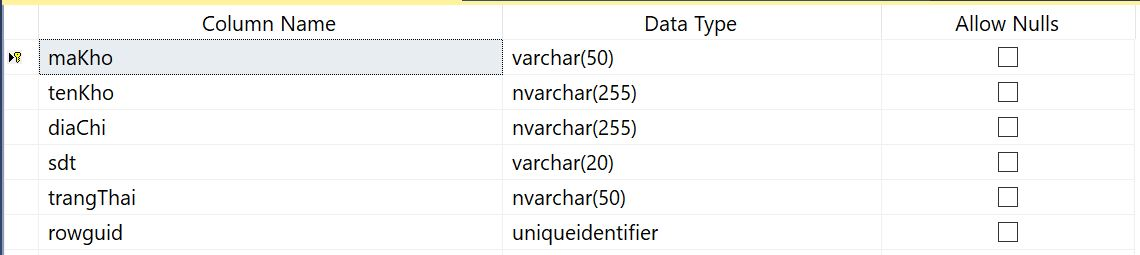
\includegraphics[width=0.8\linewidth]{image/Bao-cao-HTTTDN/Table_Kho.JPG}
    \caption{Bảng kho.}
    \label{fig:image/Bao-cao-HTTTDN/Table_Kho}
\end{figure}
\begin{figure}[H]
    \centering
    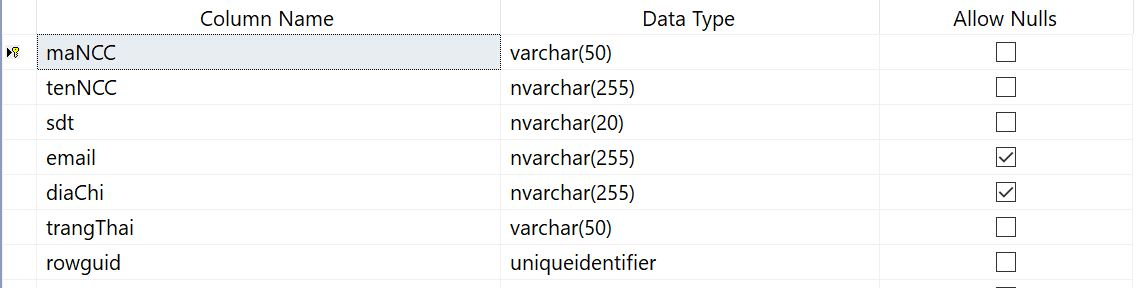
\includegraphics[width=0.8\linewidth]{image/Bao-cao-HTTTDN/Table_NCC.JPG}
    \caption{Bảng nhà cung cấp.}
    \label{fig:image/Bao-cao-HTTTDN/Table_NCC}
\end{figure}
\begin{figure}[H]
    \centering
    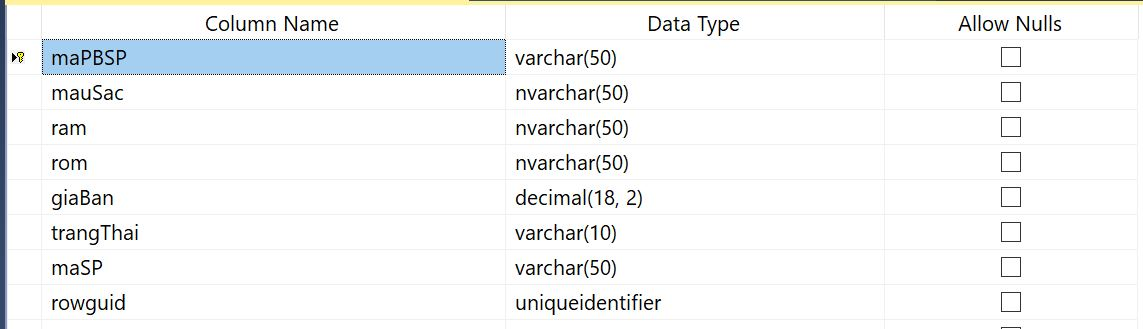
\includegraphics[width=0.8\linewidth]{image/Bao-cao-HTTTDN/Table_PBSP.JPG}
    \caption{Bảng phiên bản sản phẩm.}
    \label{fig:image/Bao-cao-HTTTDN/Table_PBSP}
\end{figure}
\begin{figure}[H]
    \centering
    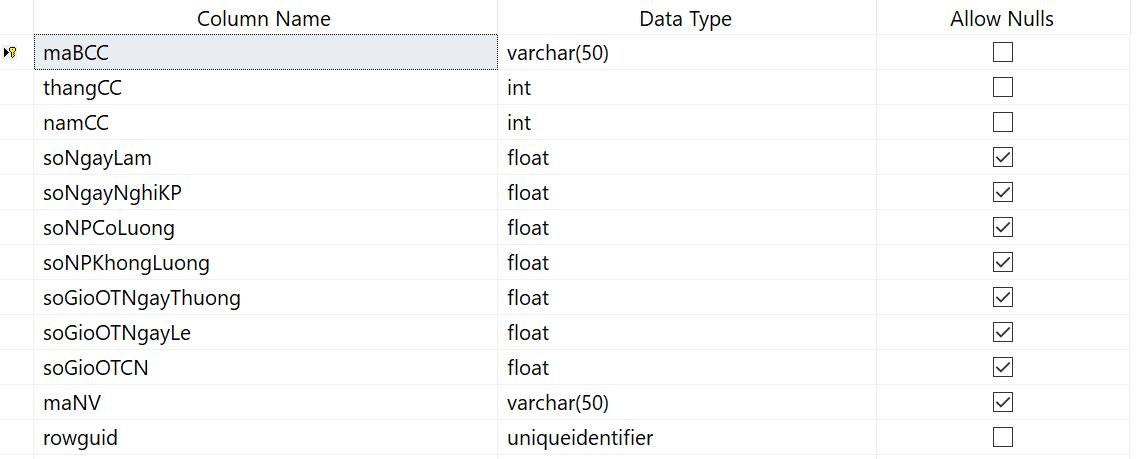
\includegraphics[width=0.8\linewidth]{image/Bao-cao-HTTTDN/Table_BangCC.JPG}
    \caption{Bảng chấm công.}
    \label{fig:image/Bao-cao-HTTTDN/Table_BangCC}
\end{figure}
\begin{figure}[H]
    \centering
    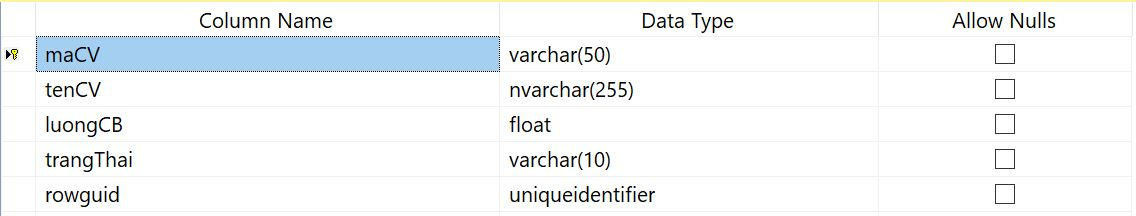
\includegraphics[width=0.8\linewidth]{image/Bao-cao-HTTTDN/Table_ChucVu.JPG}
    \caption{Bảng chức vụ.}
    \label{fig:image/Bao-cao-HTTTDN/Table_ChucVu}
\end{figure}
\begin{figure}[H]
    \centering
    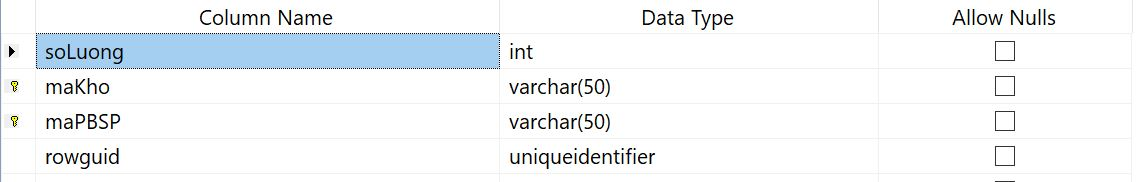
\includegraphics[width=0.8\linewidth]{image/Bao-cao-HTTTDN/Table_KhoPBSP.JPG}
    \caption{Bảng kho phiên bản sản phẩm.}
    \label{fig:image/Bao-cao-HTTTDN/Table_KhoPBSP}
\end{figure}
\begin{figure}[H]
    \centering
    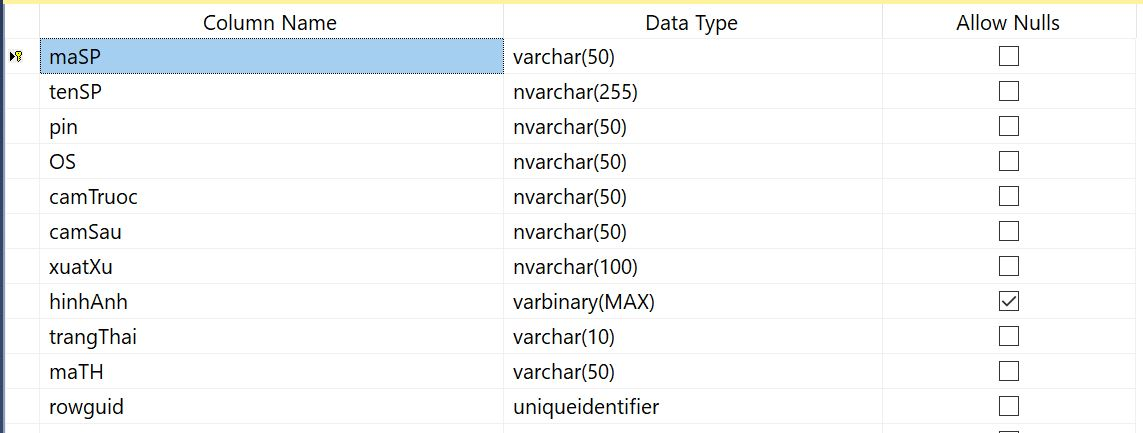
\includegraphics[width=0.8\linewidth]{image/Bao-cao-HTTTDN/Table_SanPham.JPG}
    \caption{Bảng sản phẩm.}
    \label{fig:image/Bao-cao-HTTTDN/Table_SanPham}
\end{figure}
\begin{figure}[H]
    \centering
    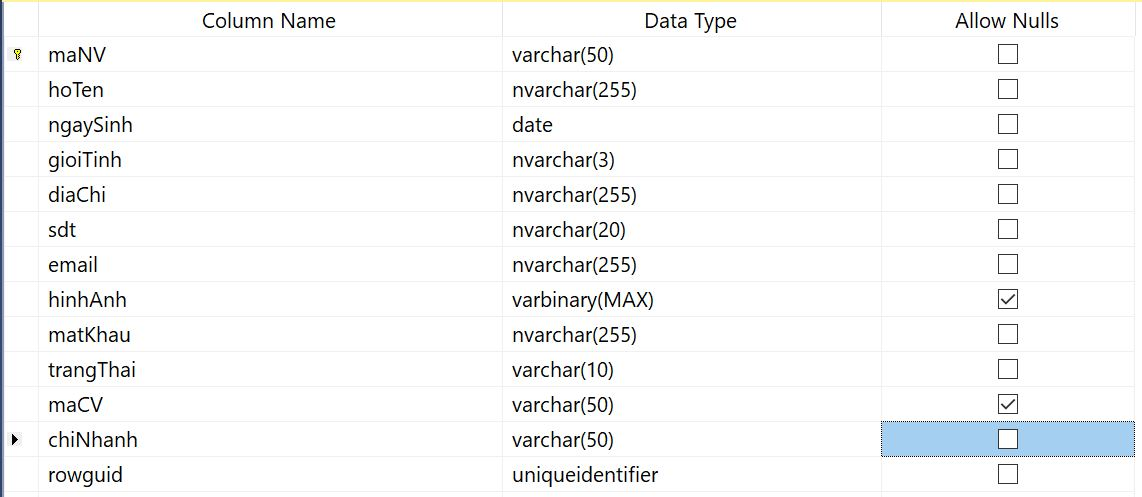
\includegraphics[width=0.8\linewidth]{image/Bao-cao-HTTTDN/Table_NhanVien.JPG}
    \caption{Bảng nhân viên.}
    \label{fig:image/Bao-cao-HTTTDN/Table_NhanVien}
\end{figure}

\begin{figure}[H]
    \centering
    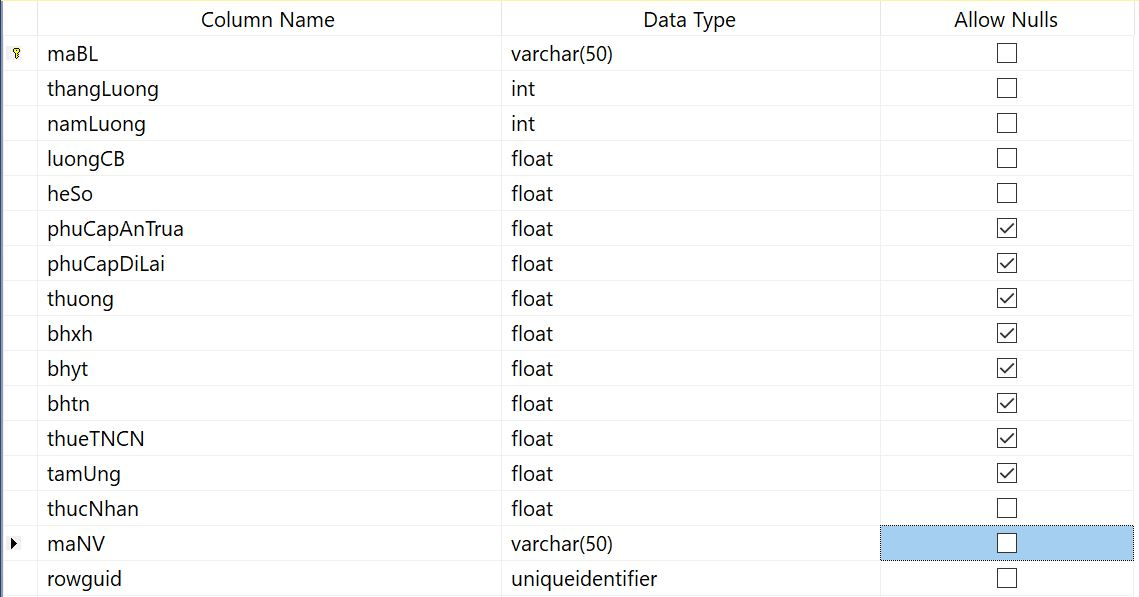
\includegraphics[width=0.8\linewidth]{image/Bao-cao-HTTTDN/Table_BangLuong.JPG}
    \caption{Bảng lương.}
    \label{fig:image/Bao-cao-HTTTDN/Table_BangLuong}
\end{figure}
\begin{figure}[H]
    \centering
    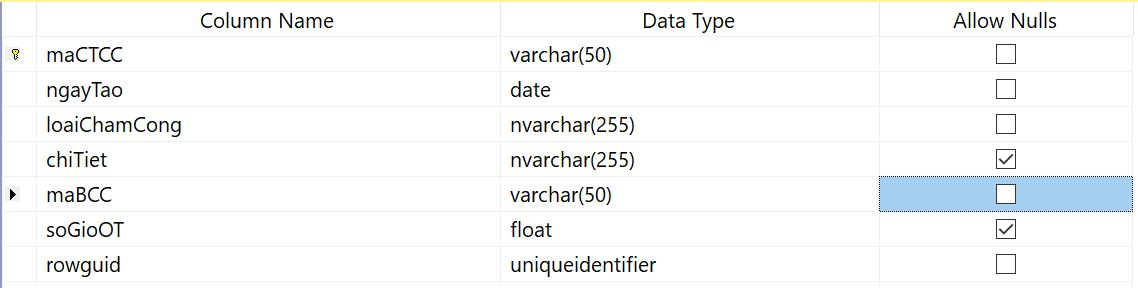
\includegraphics[width=0.8\linewidth]{image/Bao-cao-HTTTDN/Table_ChiTietCC.JPG}
    \caption{Bảng chi tiết chấm công.}
    \label{fig:image/Bao-cao-HTTTDN/Table_ChiTietCC}
\end{figure}
\begin{figure}[H]
    \centering
    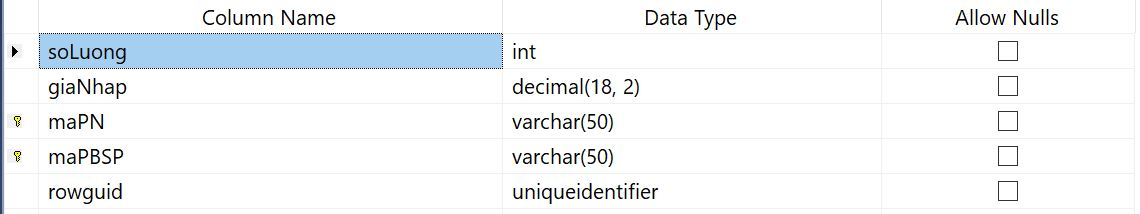
\includegraphics[width=0.8\linewidth]{image/Bao-cao-HTTTDN/Table_ChiTietPN.JPG}
    \caption{Bảng chi tiết phiếu nhập.}
    \label{fig:image/Bao-cao-HTTTDN/Table_ChiTietPN}
\end{figure}
\begin{figure}[H]
    \centering
    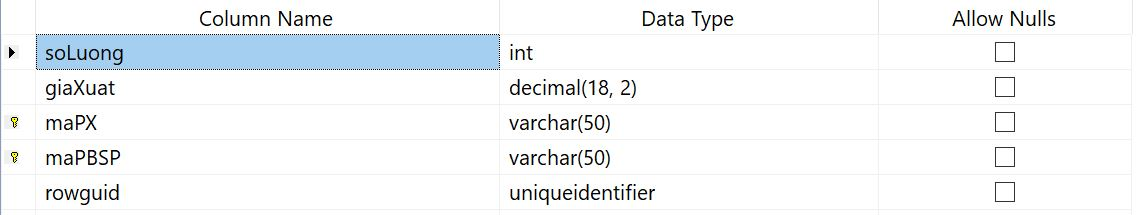
\includegraphics[width=0.8\linewidth]{image/Bao-cao-HTTTDN/Table_ChiTietPX.JPG}
    \caption{Bảng chi tiết phiếu xuất.}
    \label{fig:image/Bao-cao-HTTTDN/Table_ChiTietPX}
\end{figure}
\begin{figure}[H]
    \centering
    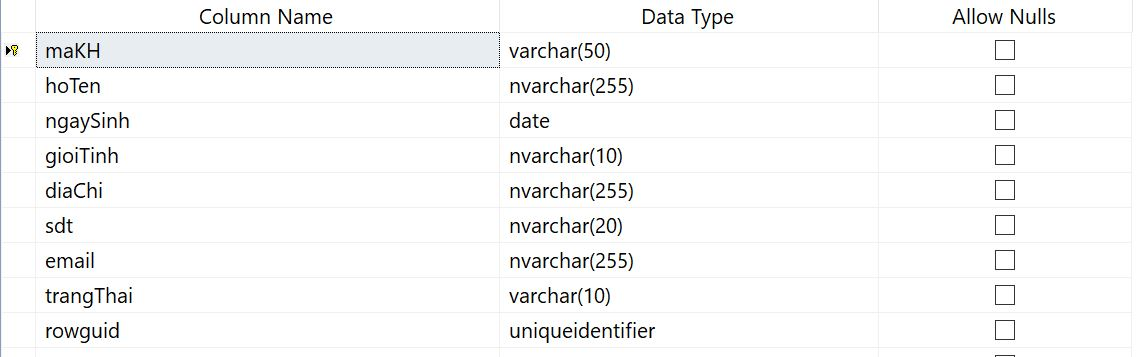
\includegraphics[width=0.8\linewidth]{image/Bao-cao-HTTTDN/Table_KhachHang.JPG}
    \caption{Bảng khách hàng.}
    \label{fig:image/Bao-cao-HTTTDN/Table_KhachHang}
\end{figure}
\begin{figure}[H]
    \centering
    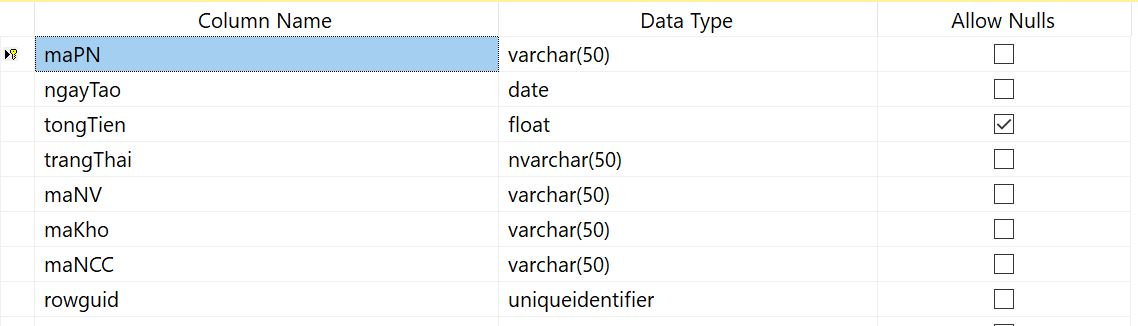
\includegraphics[width=0.8\linewidth]{image/Bao-cao-HTTTDN/Table_PhieuNhap.JPG}
    \caption{Bảng phiếu nhập.}
    \label{fig:image/Bao-cao-HTTTDN/Table_PhieuNhap}
\end{figure}
\begin{figure}[H]
    \centering
    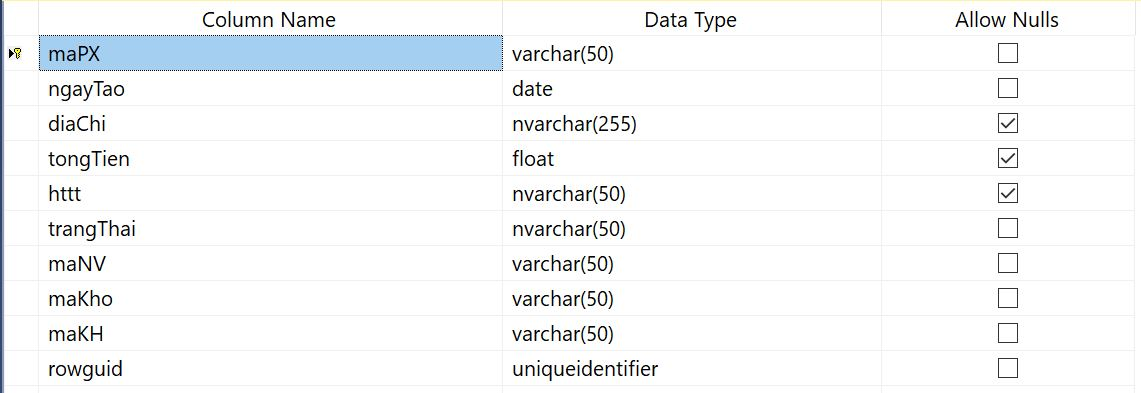
\includegraphics[width=0.8\linewidth]{image/Bao-cao-HTTTDN/Table_PhieuXuat.JPG}
    \caption{Bảng phiếu xuất.}
    \label{fig:image/Bao-cao-HTTTDN/Table_PhieuXuat}
\end{figure}
\begin{figure}[H]
    \centering
    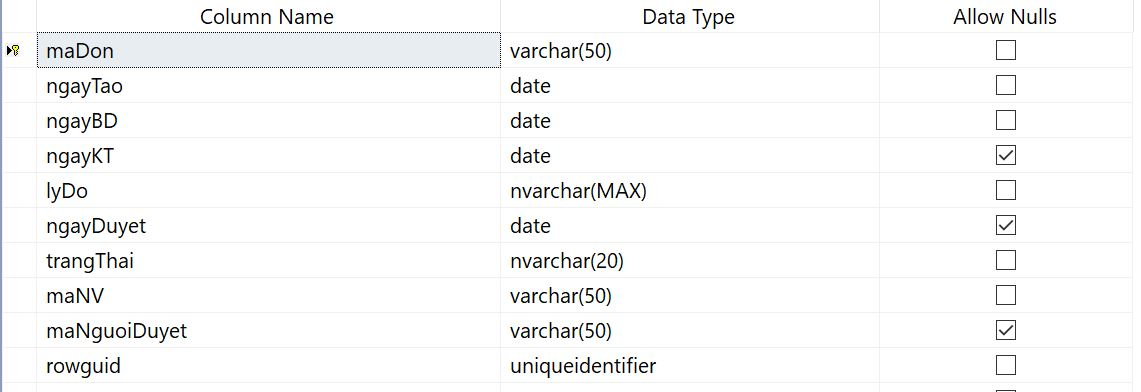
\includegraphics[width=0.8\linewidth]{image/Bao-cao-HTTTDN/Table_DonXinNghi.JPG}
    \caption{Bảng đơn xin nghỉ.}
    \label{fig:image/Bao-cao-HTTTDN/Table_DonXinNghi}
\end{figure}
\begin{figure}[H]
    \centering
    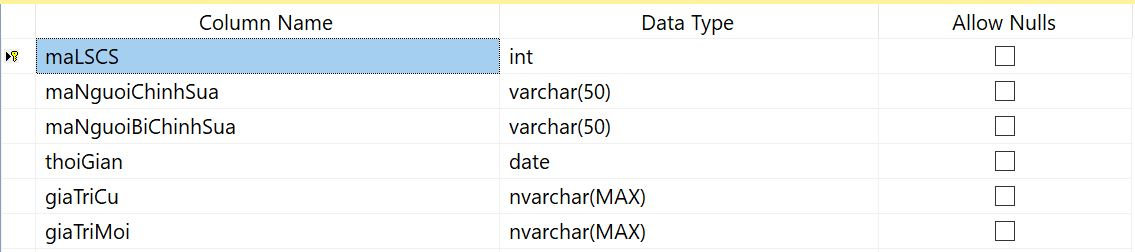
\includegraphics[width=0.8\linewidth]{image/Bao-cao-HTTTDN/Table_LSChinhSua.JPG}
    \caption{Bảng lịch sử chỉnh sửa.}
    \label{fig:image/Bao-cao-HTTTDN/Table_LSChinhSua}
\end{figure}
\begin{figure}[H]
    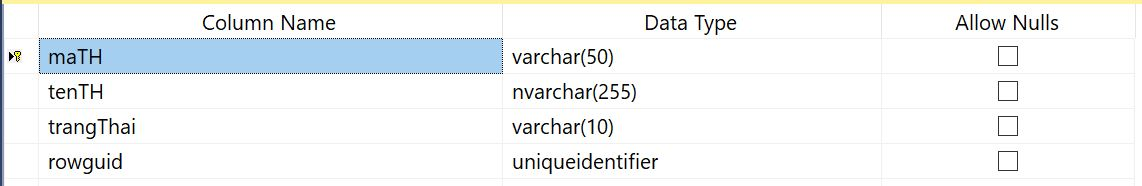
\includegraphics[width=0.8\linewidth]{image/Bao-cao-HTTTDN/Table_ThuongHieu.JPG}
    \caption{Bảng thương hiệu.}
    \label{fig:image/Bao-cao-HTTTDN/Table_ThuongHieu}
\end{figure}
\section{Các giao diện của phần mềm}
\begin{figure}[H]
    \centering
    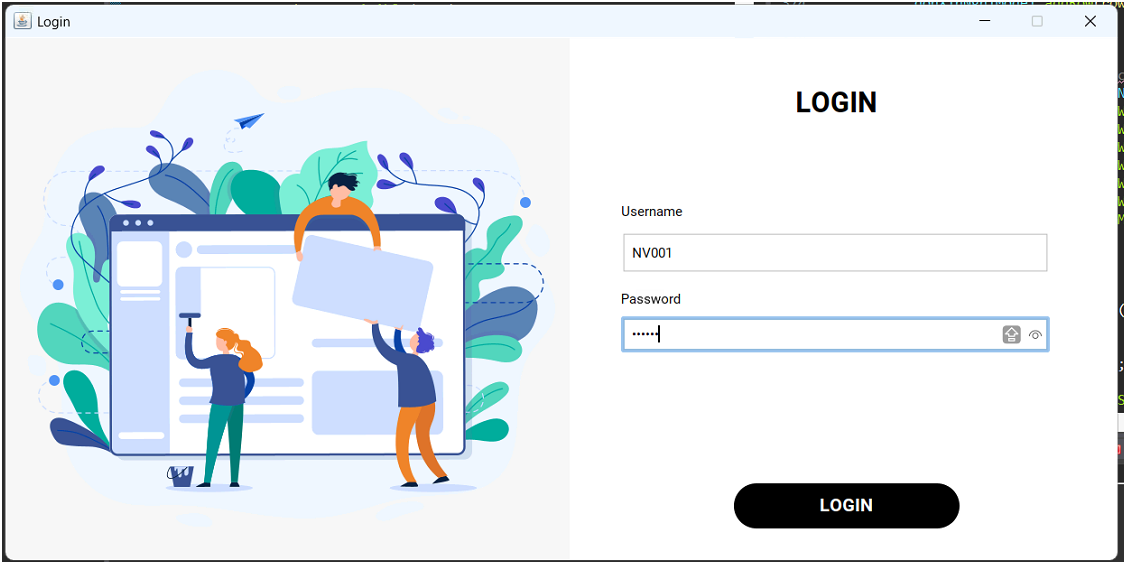
\includegraphics[width=0.8\linewidth]{image/Bao-cao-HTTTDN/giaodien-login.png}
    \caption{Giao diện đăng nhập.}
    \label{fig:image/Bao-cao-HTTTDN/giaodien-login}
\end{figure}
\begin{figure}[H]
    \centering
    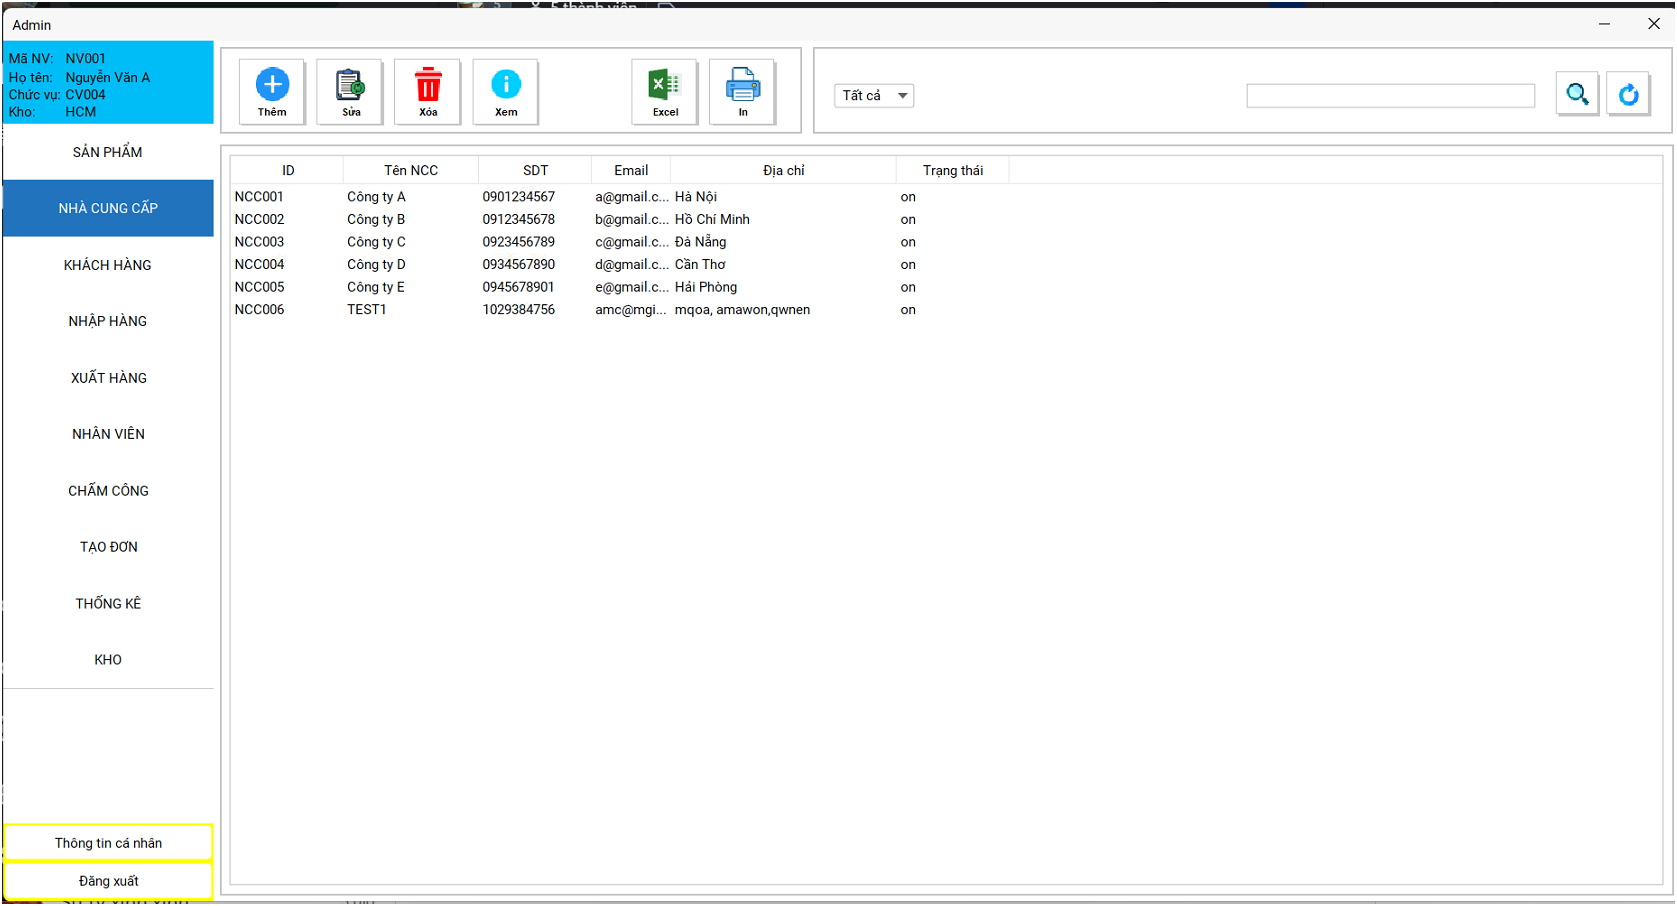
\includegraphics[width=0.8\linewidth]{image/Bao-cao-HTTTDN/giaodien-nhacungcap.png}
    \caption{Giao diện nhà cung cấp.}
    \label{fig:image/Bao-cao-HTTTDN/giaodien-nhacungcap}
\end{figure}
\begin{figure}[H]
    \centering
    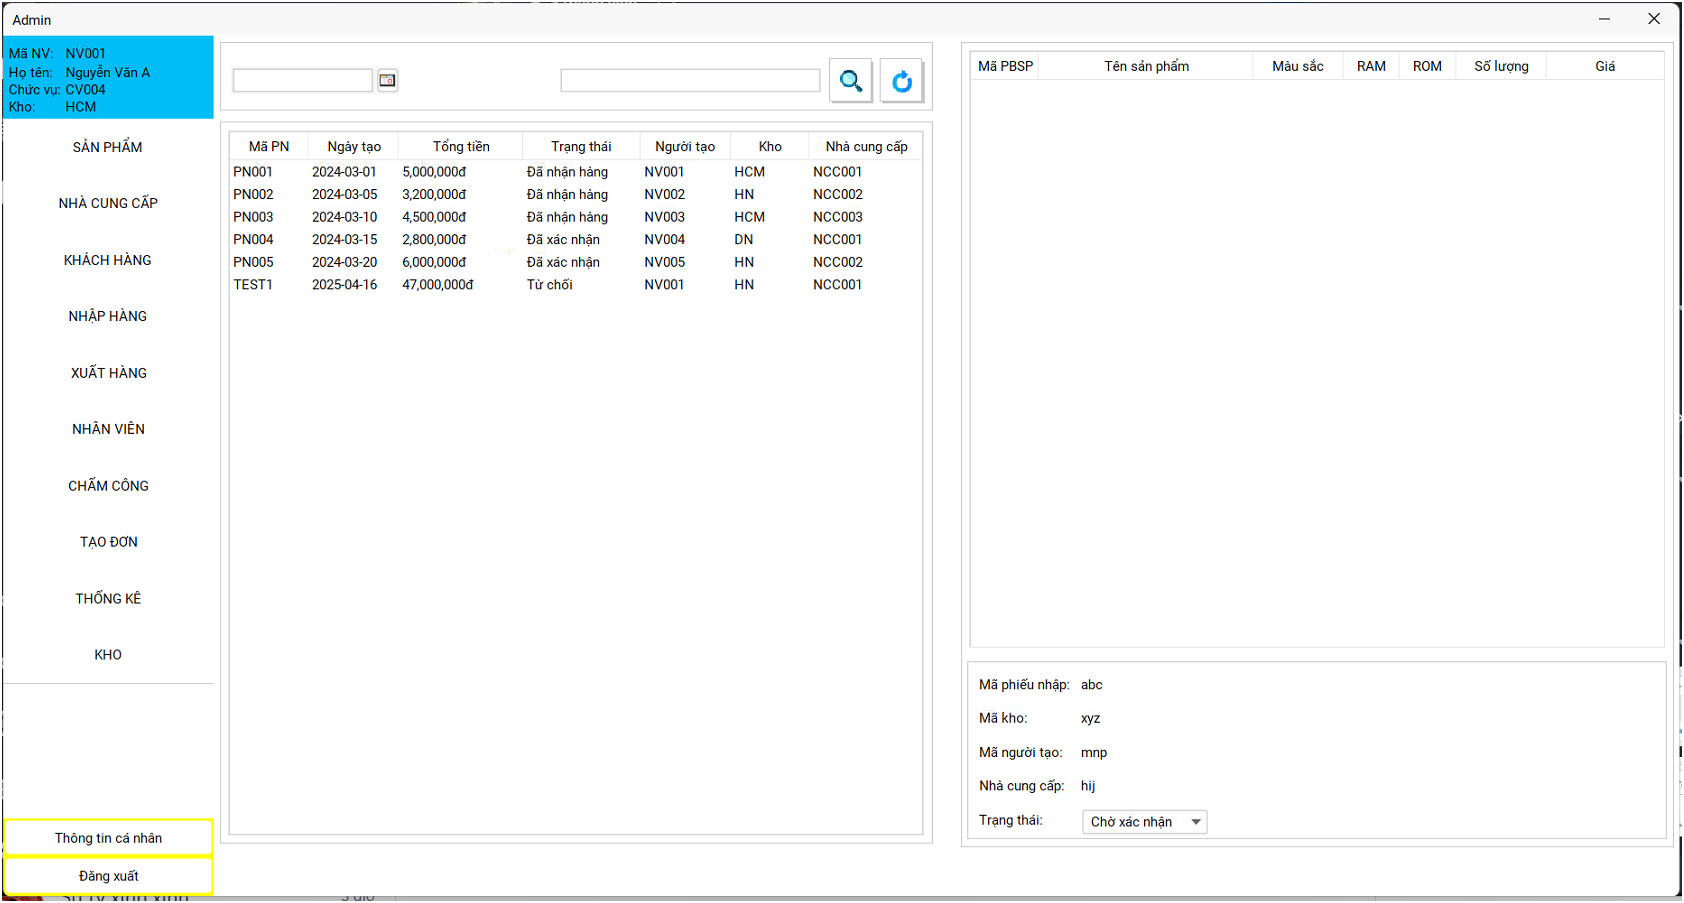
\includegraphics[width=0.8\linewidth]{image/Bao-cao-HTTTDN/giaodien-phieunhap.png}
    \caption{Giao diện phiếu nhập.}
    \label{fig:image/Bao-cao-HTTTDN/giaodien-phieunhap}
\end{figure}
\begin{figure}[H]
    \centering
    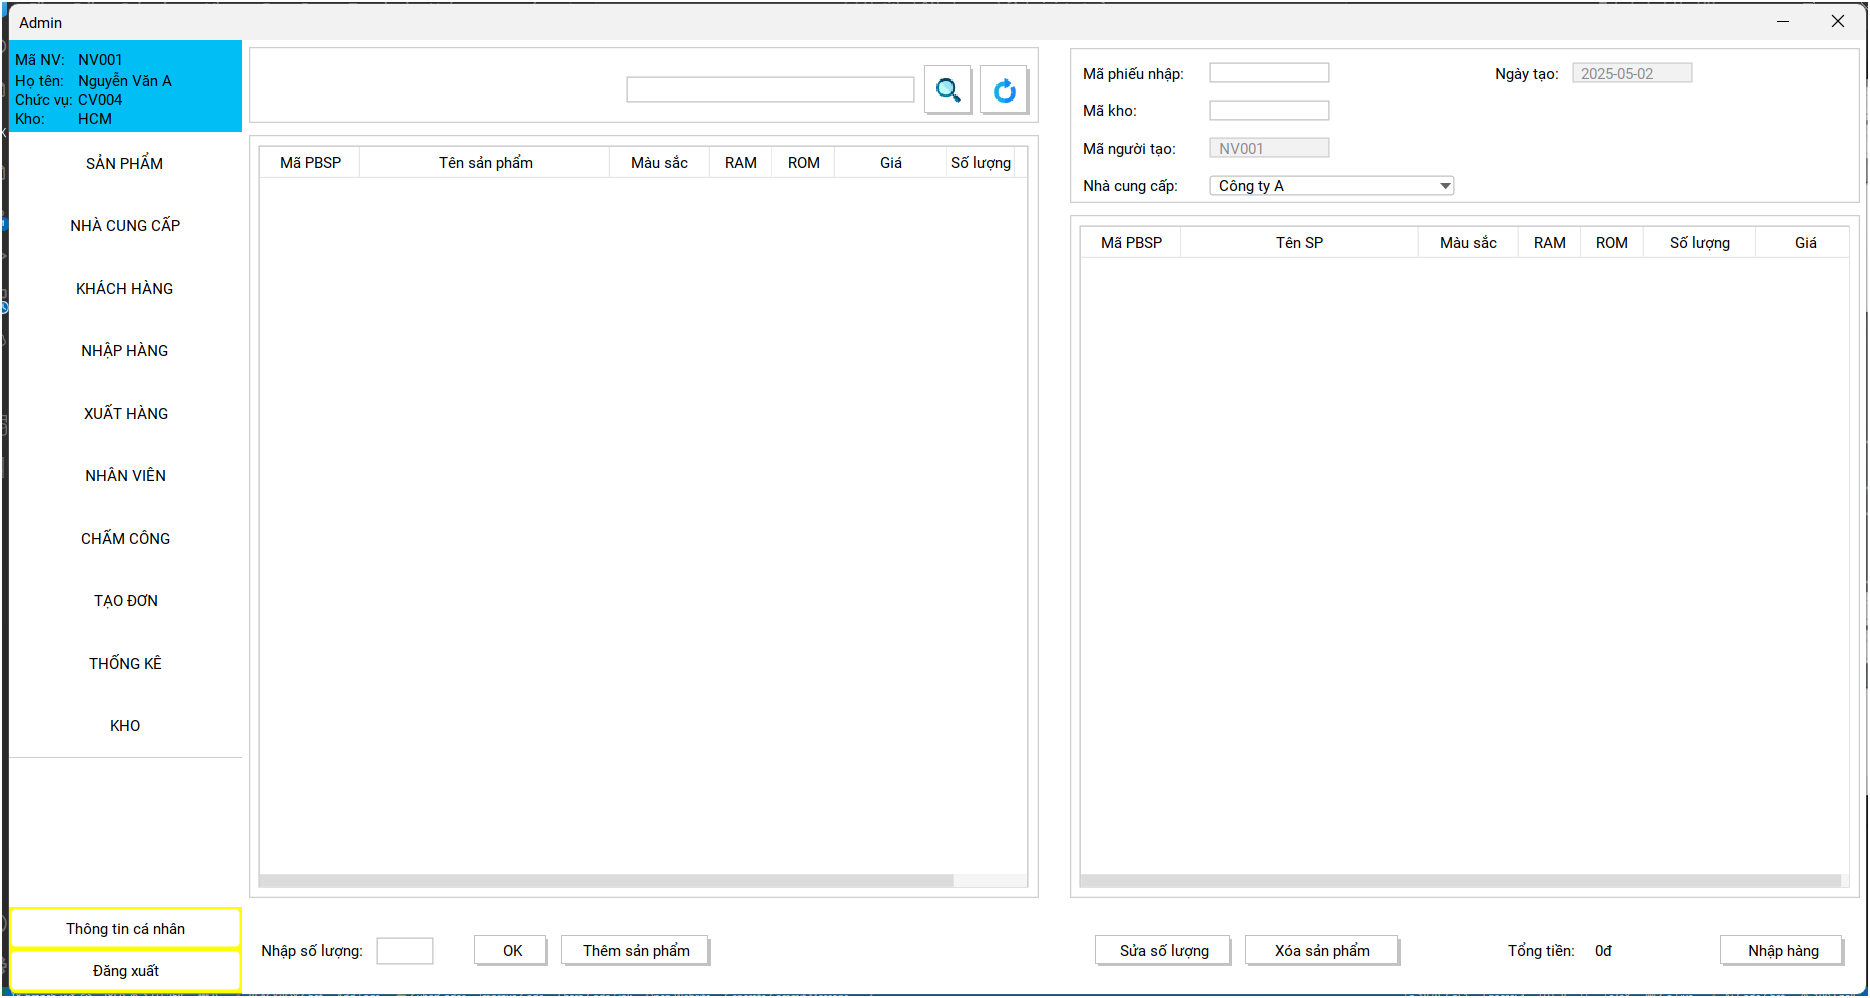
\includegraphics[width=0.8\linewidth]{image/Bao-cao-HTTTDN/giaodien-taophieunhap.png}
    \caption{Giao diện tạo phiếu nhập.}
    \label{fig:image/Bao-cao-HTTTDN/giaodien-taophieunhap}
\end{figure}
\begin{figure}[H]
    \centering
    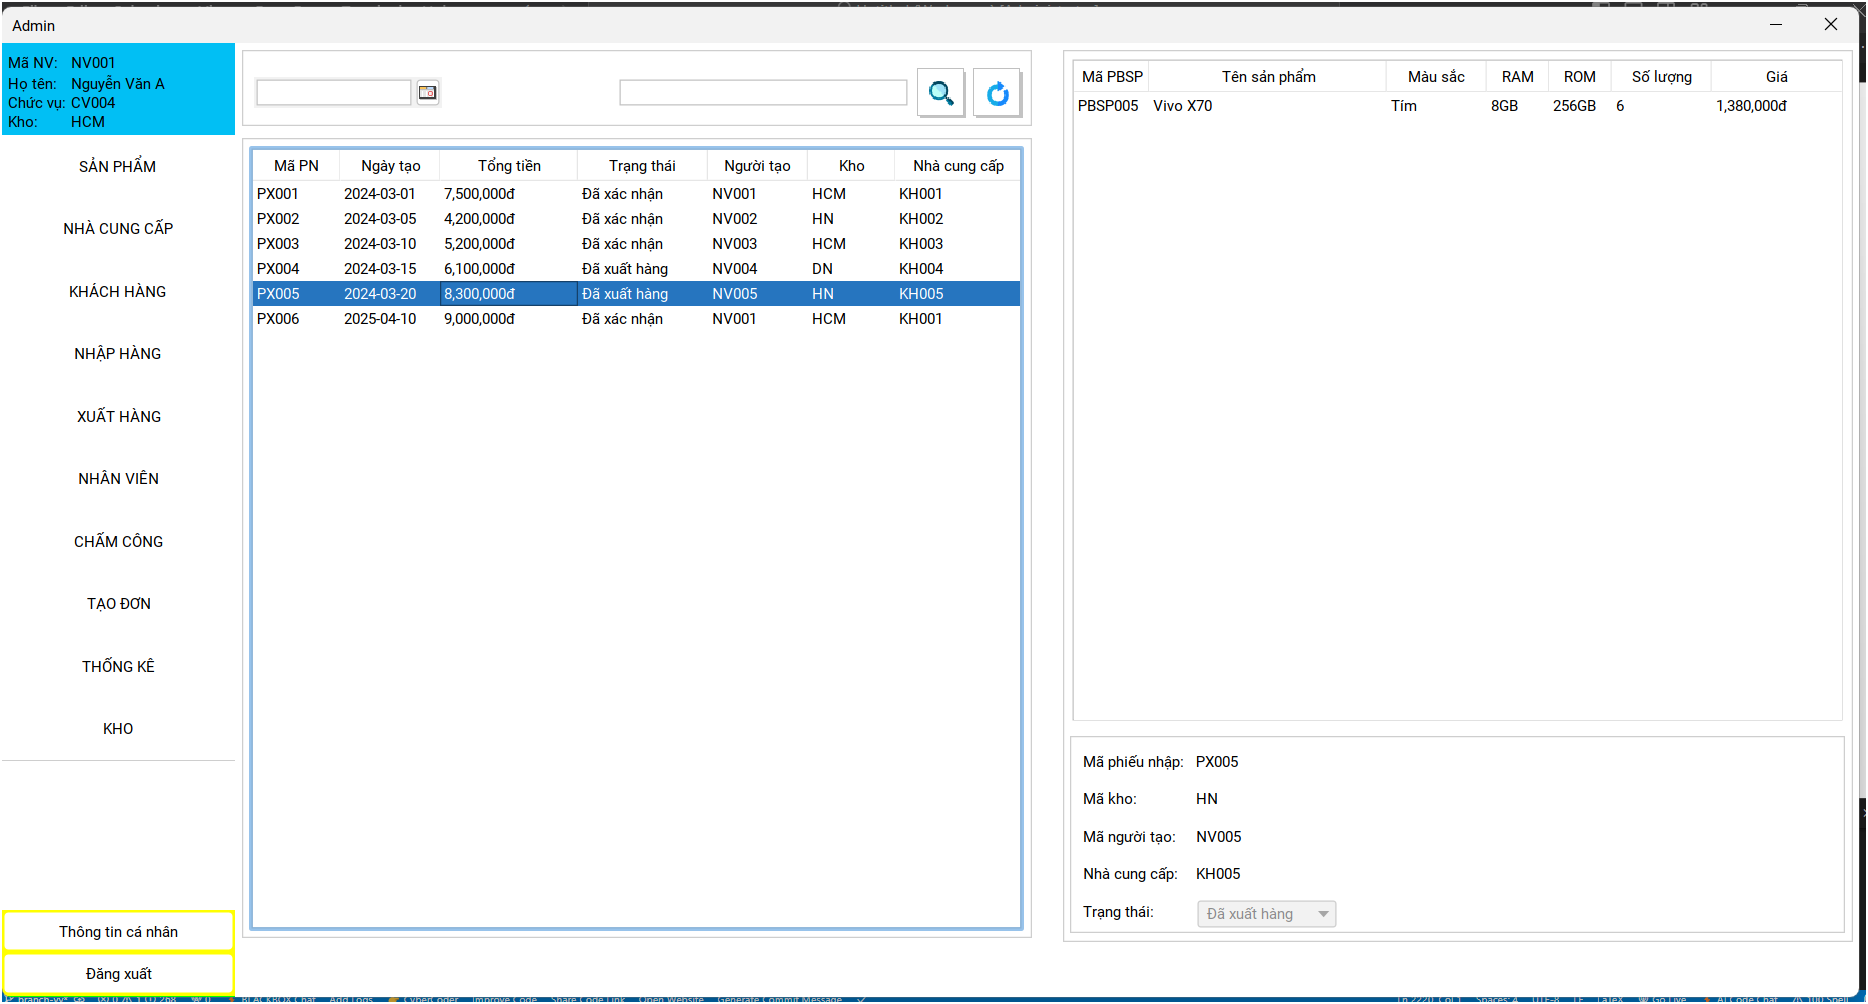
\includegraphics[width=0.8\linewidth]{image/Bao-cao-HTTTDN/giaodien-xuathang.png}
    \caption{Giao diện xuất hàng.}
    \label{fig:image/Bao-cao-HTTTDN/giaodien-xuathang}
\end{figure}
\begin{figure}[H]
    \centering
    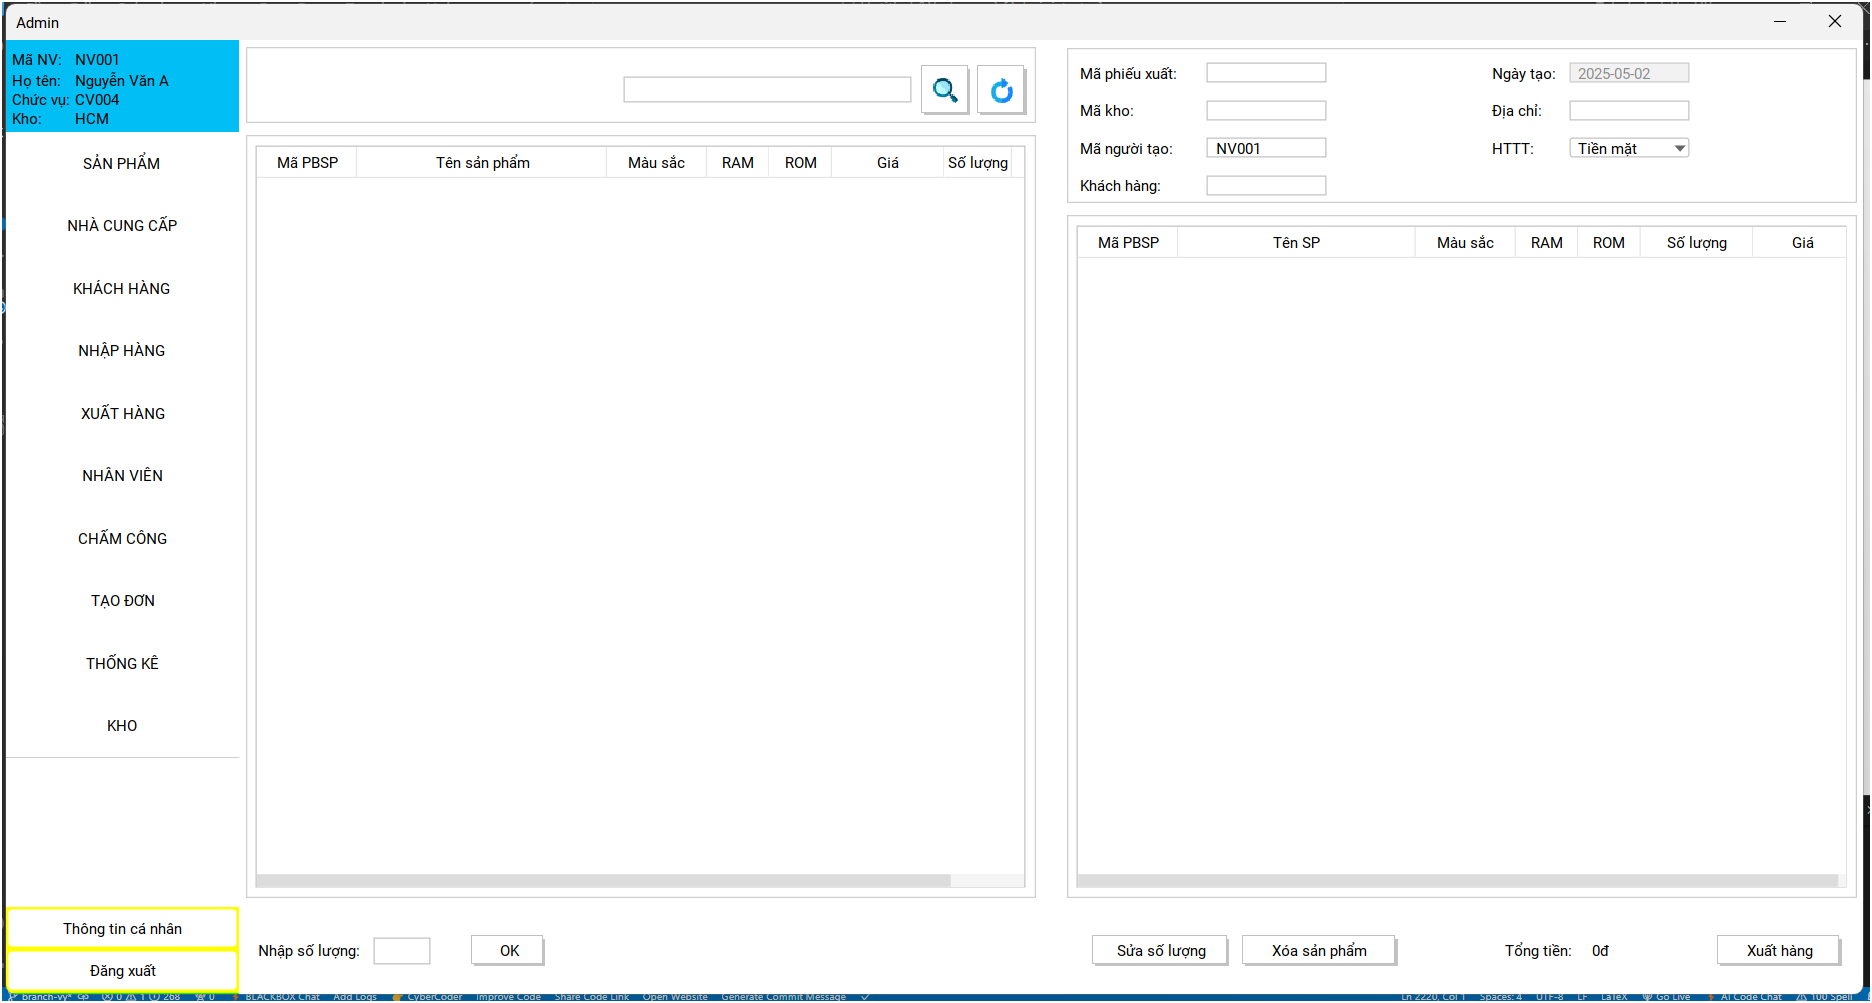
\includegraphics[width=0.8\linewidth]{image/Bao-cao-HTTTDN/giaodien-taoXuatHang.png}
    \caption{Giao diện tạo xuất hàng.}
    \label{fig:image/Bao-cao-HTTTDN/giaodien-taoXuatHang}
\end{figure}
\begin{figure}[H]
    \centering
    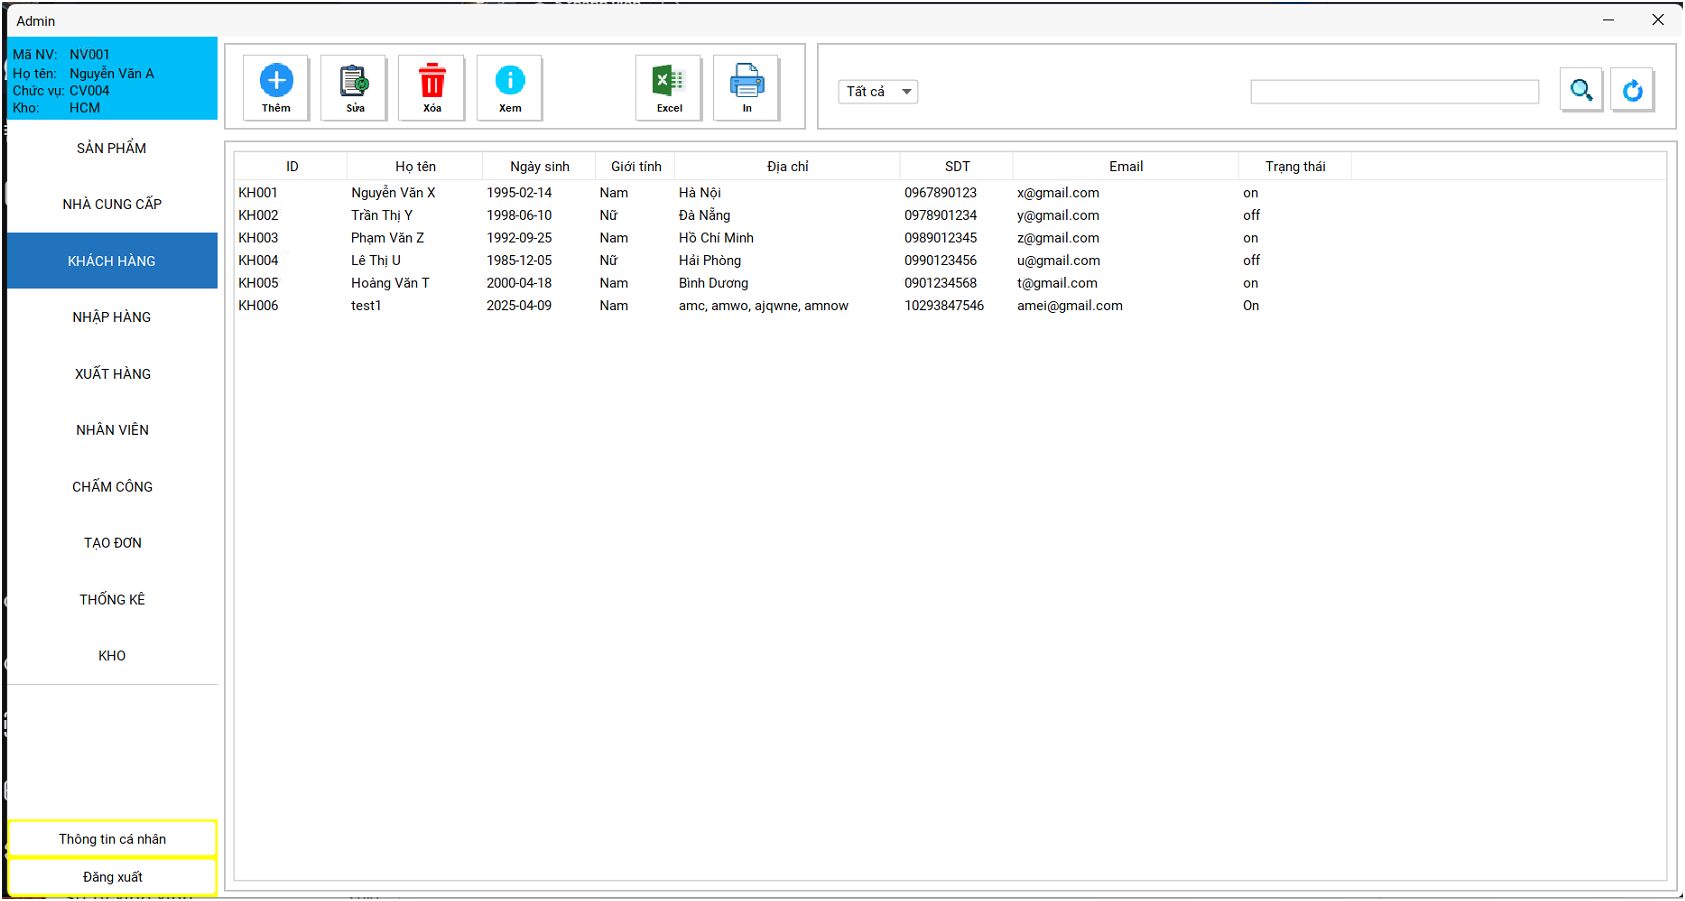
\includegraphics[width=0.8\linewidth]{image/Bao-cao-HTTTDN/giaodien-khachhang.png}
    \caption{Giao diện khách hàng.}
    \label{fig:image/Bao-cao-HTTTDN/giaodien-khachhang}
\end{figure}
\begin{figure}[H]
    \centering
    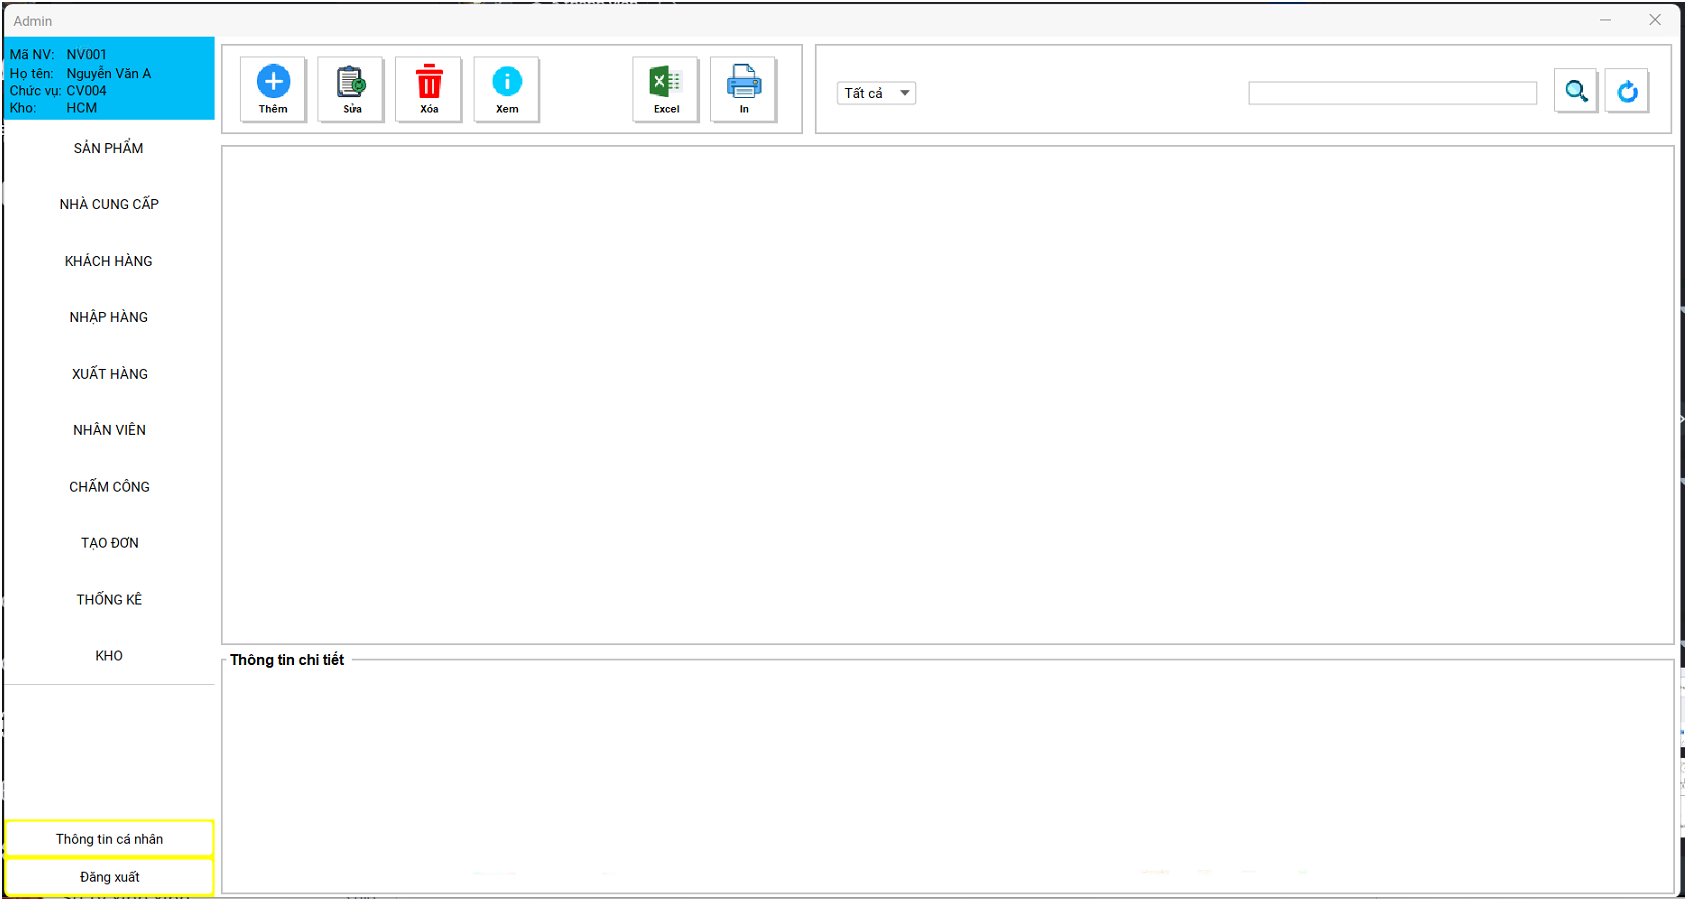
\includegraphics[width=0.8\linewidth]{image/Bao-cao-HTTTDN/giaodien-chamcong.png}
    \caption{Giao diện danh sách lương.}
    \label{fig:image/Bao-cao-HTTTDN/giaodien-chamcong}
\end{figure}
\begin{figure}[H]
    \centering
    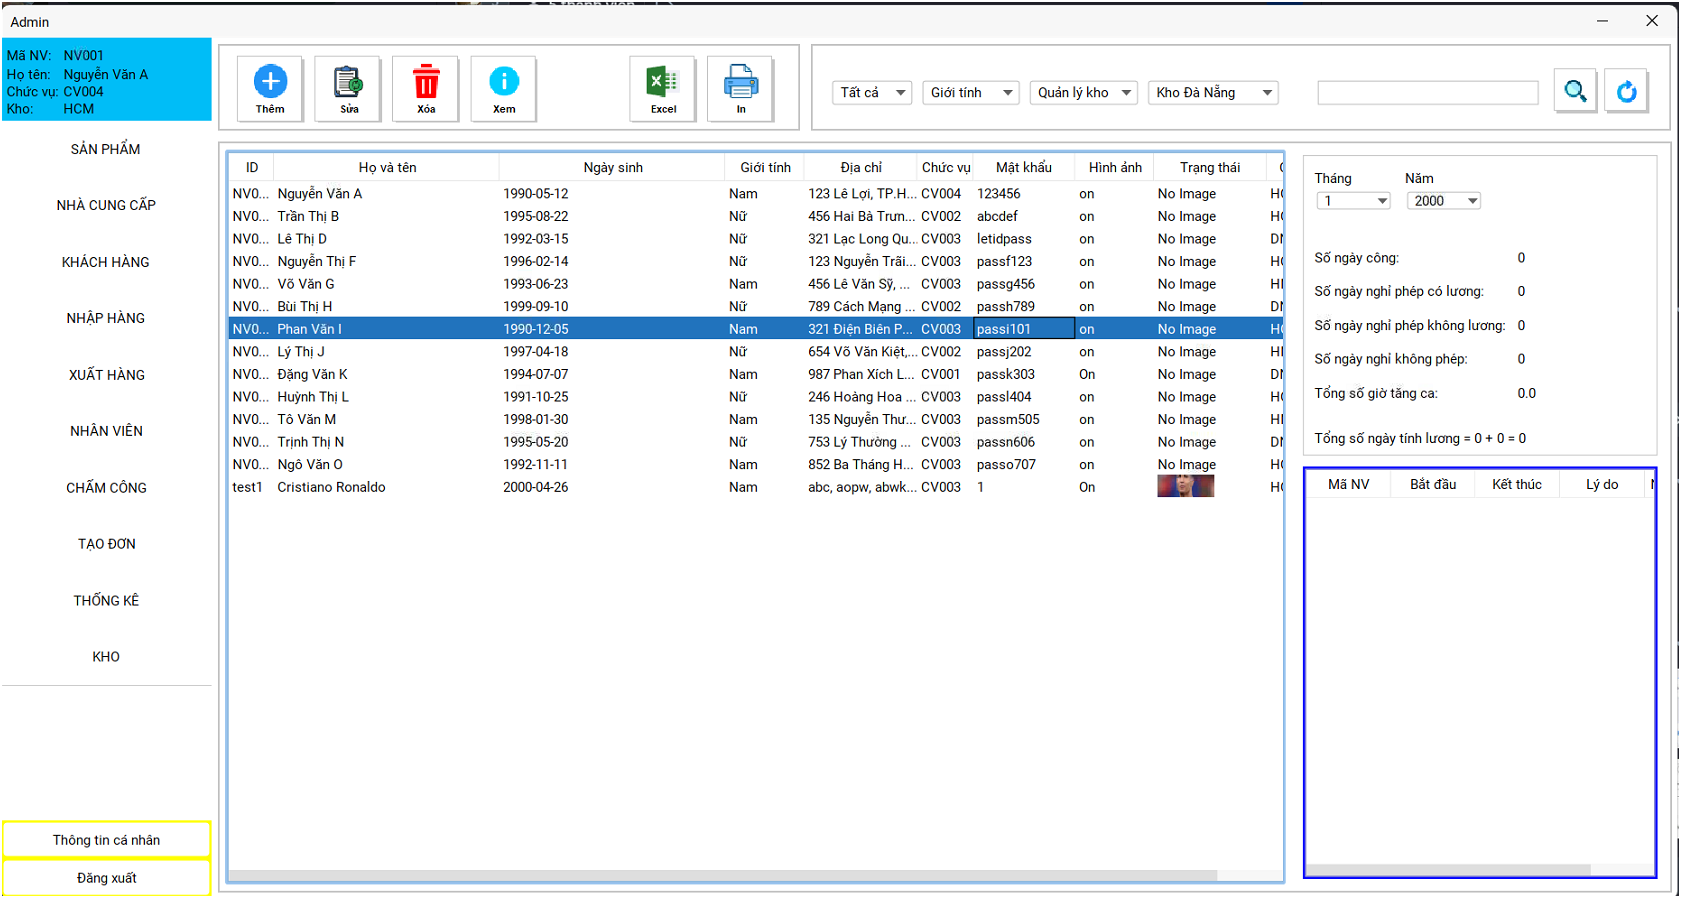
\includegraphics[width=0.8\linewidth]{image/Bao-cao-HTTTDN/giaodien-danhsachnv.png}
    \caption{Giao diện danh sách nhân viên.}
    \label{fig:image/Bao-cao-HTTTDN/giaodien-danhsachnv}
\end{figure}
\begin{figure}[H]
    \centering
    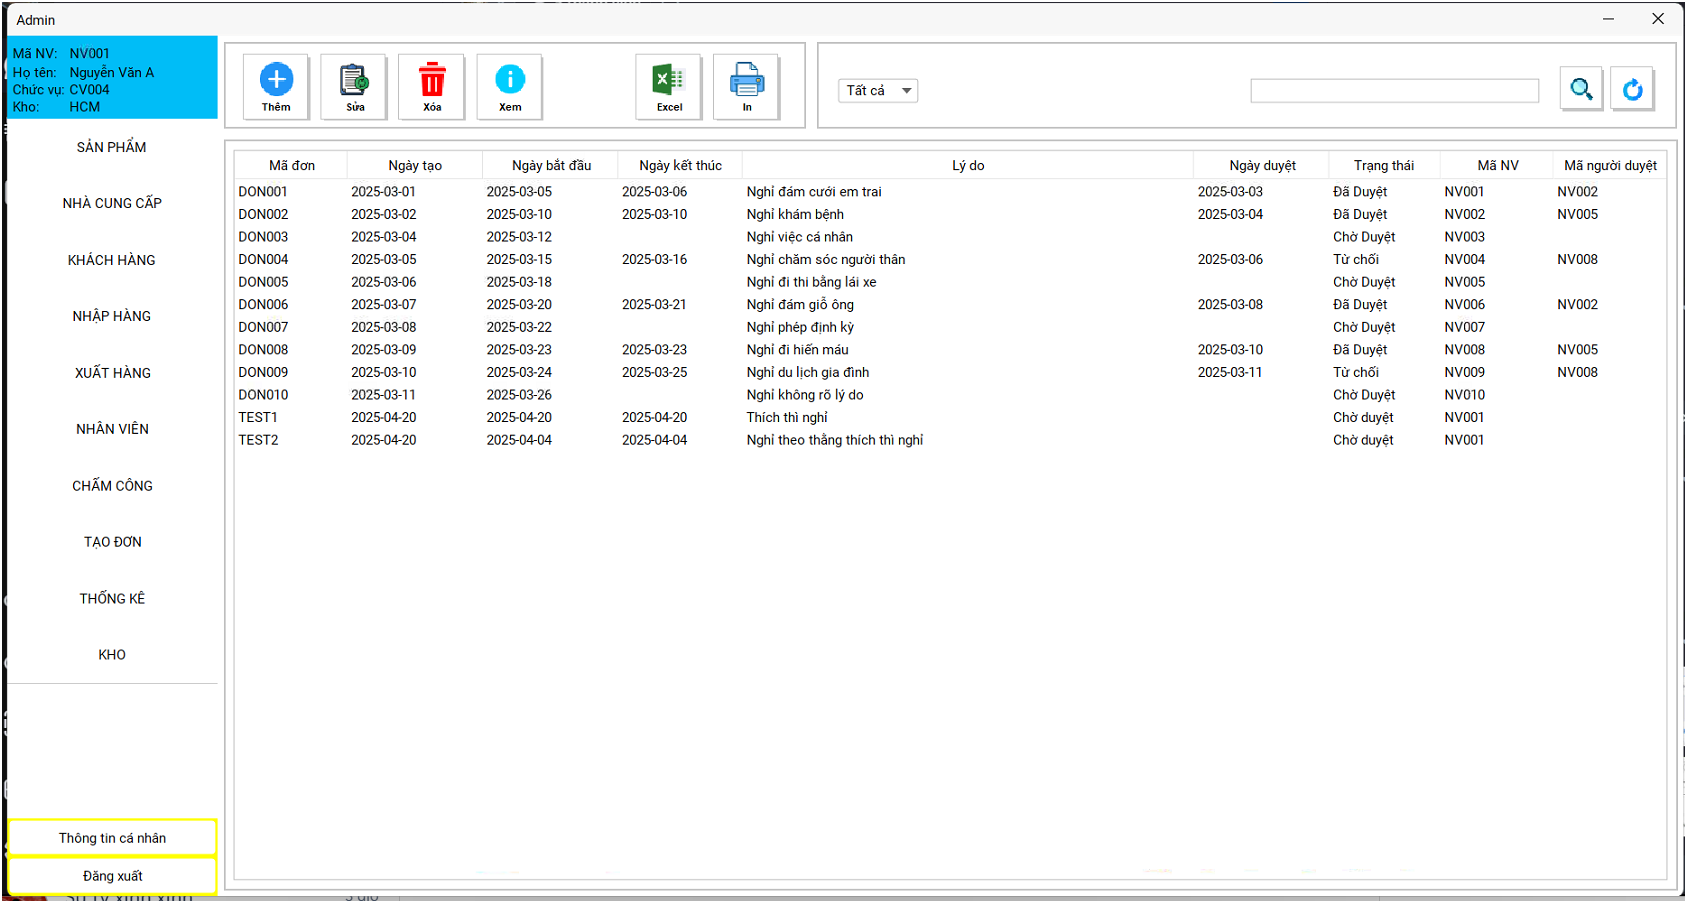
\includegraphics[width=0.8\linewidth]{image/Bao-cao-HTTTDN/giaodien-danhsachdonxin.png}
    \caption{Giao diện danh sách đơn xin nghỉ.}
    \label{fig:image/Bao-cao-HTTTDN/giaodien-danhsachdonxin}
\end{figure}
\begin{figure}[H]
    \centering
    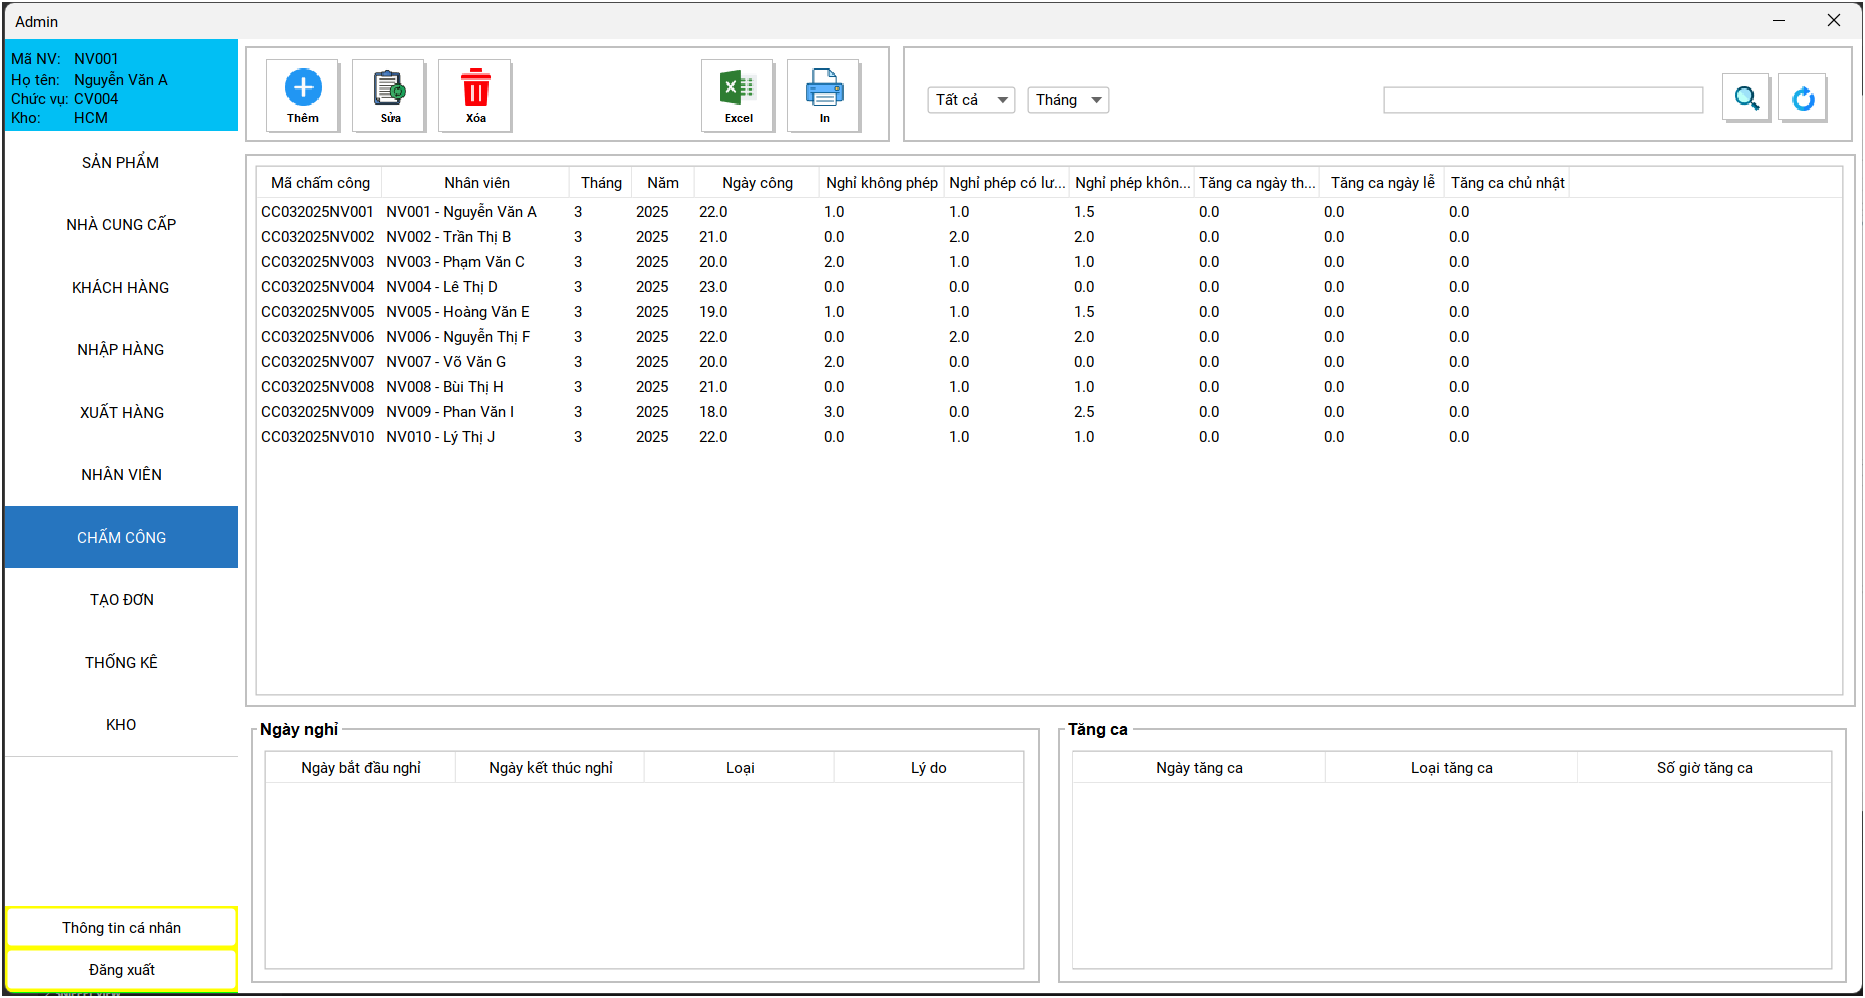
\includegraphics[width=0.8\linewidth]{image/Bao-cao-HTTTDN/giaodien-nvchamcong.png}
    \caption{Giao diện chấm công.}
    \label{fig:image/Bao-cao-HTTTDN/giaodien-nvchamcong}
\end{figure}
\begin{figure}[H]
    \centering
    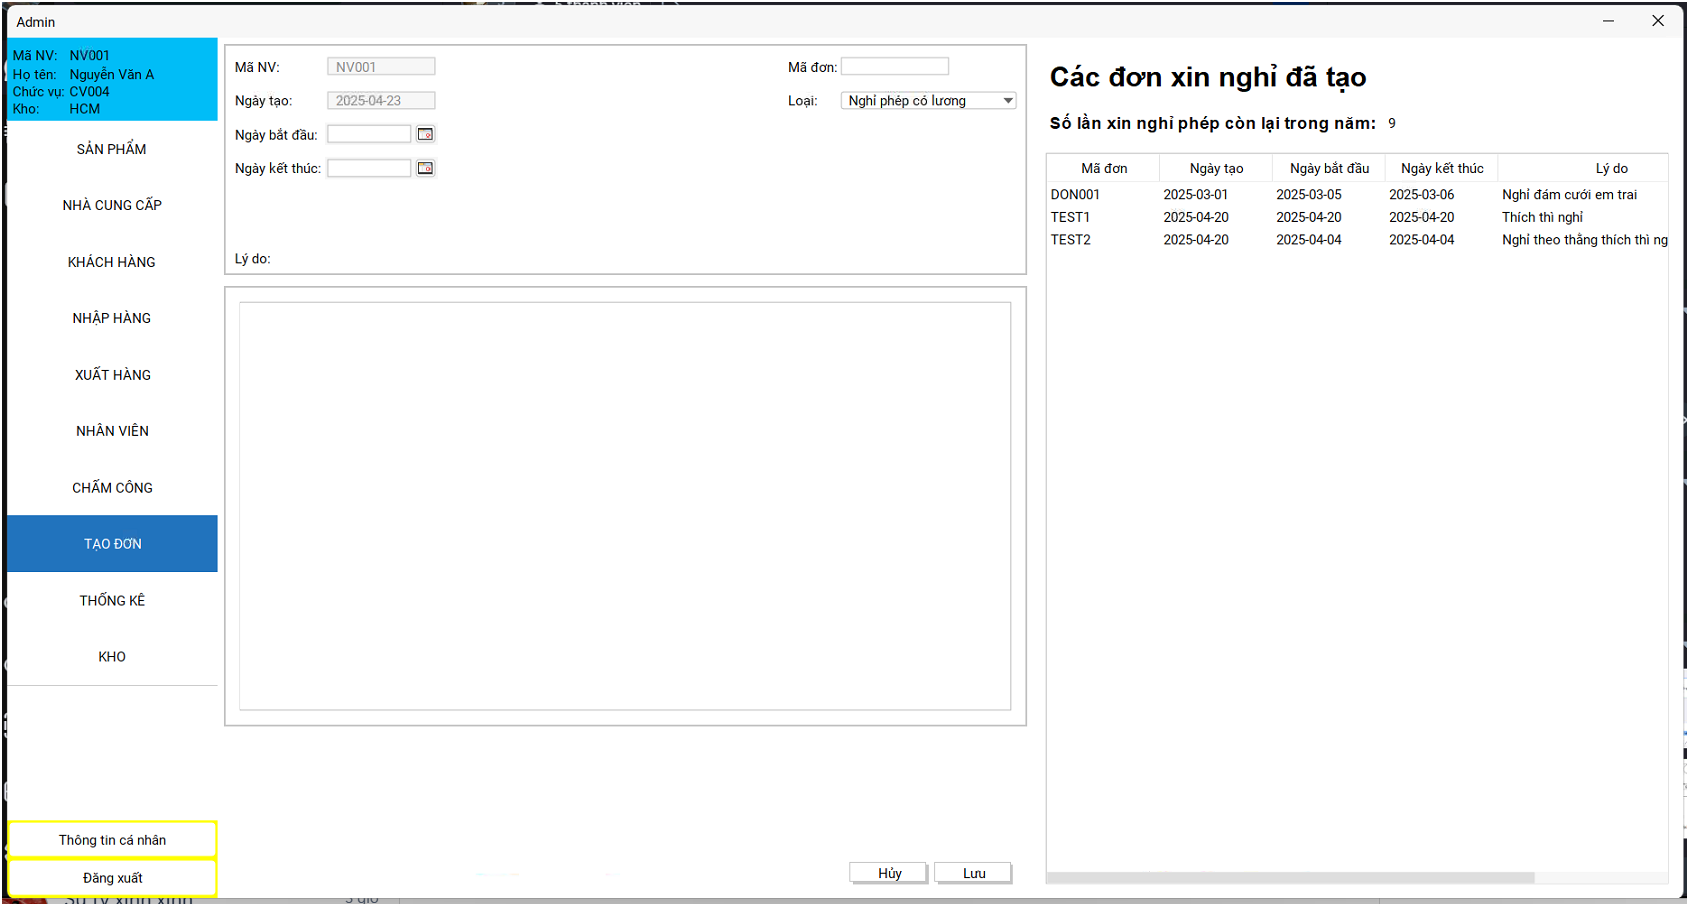
\includegraphics[width=0.8\linewidth]{image/Bao-cao-HTTTDN/giaodien-taodon.png}
    \caption{Giao diện tạo đơn nghỉ.}
    \label{fig:image/Bao-cao-HTTTDN/giaodien-taodon}
\end{figure}
\begin{figure}[H]
    \centering
    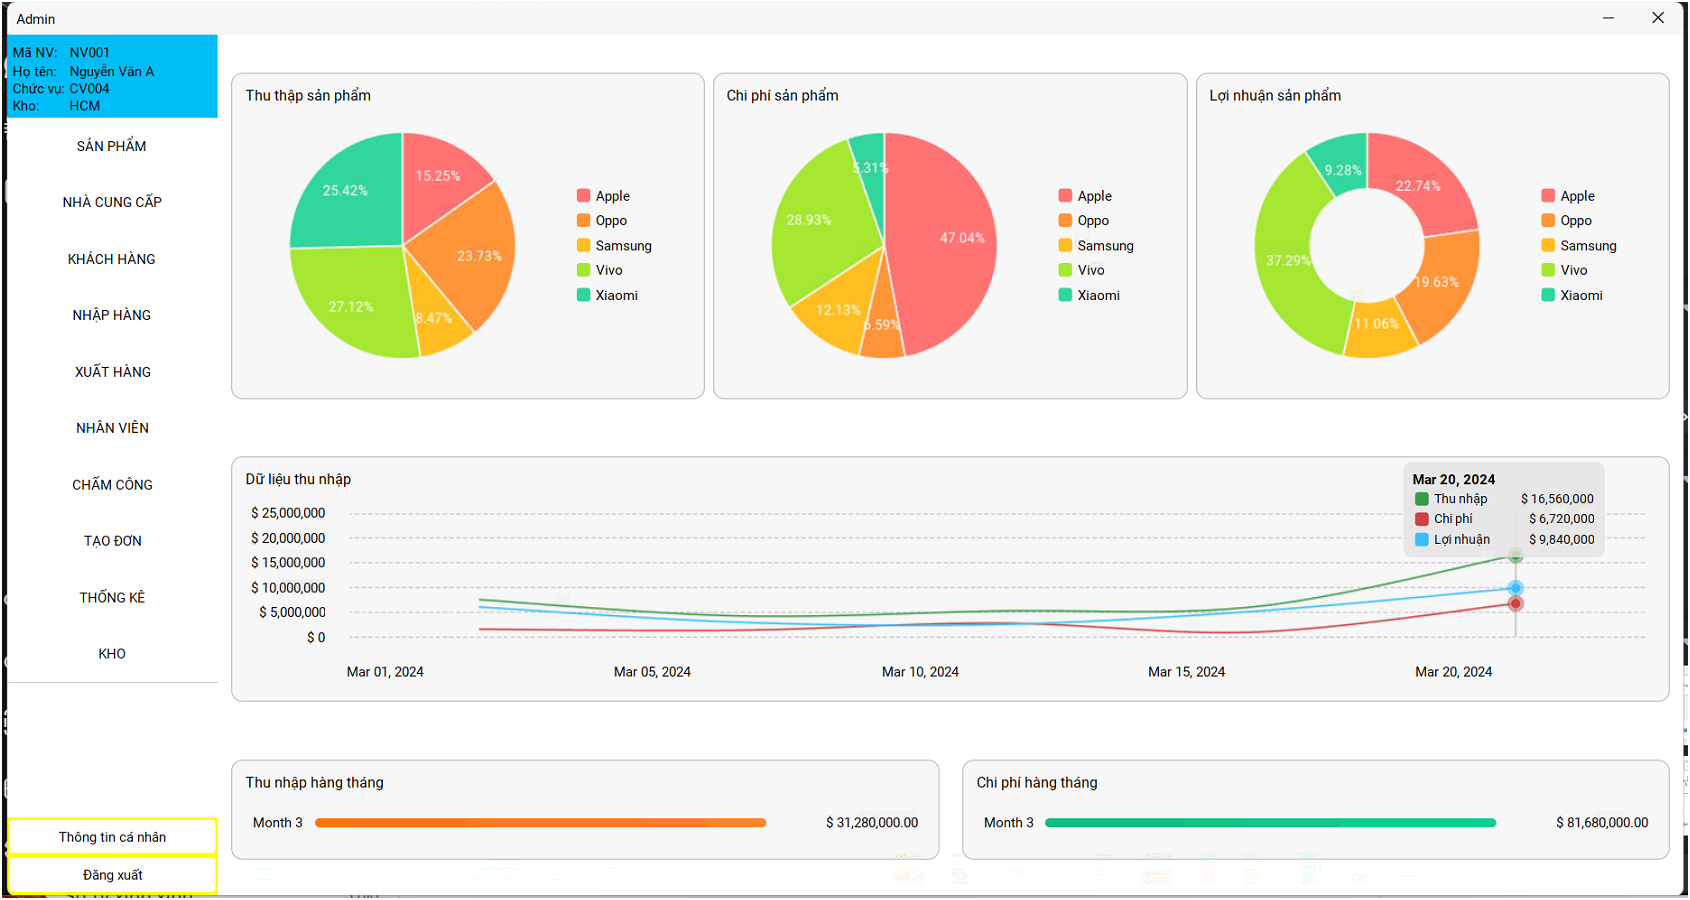
\includegraphics[width=0.8\linewidth]{image/Bao-cao-HTTTDN/giaodien-thongke.png}
    \caption{Giao diện thống kê.}
    \label{fig:image/Bao-cao-HTTTDN/giaodien-thongke}
\end{figure}
\begin{figure}[H]
    \centering
    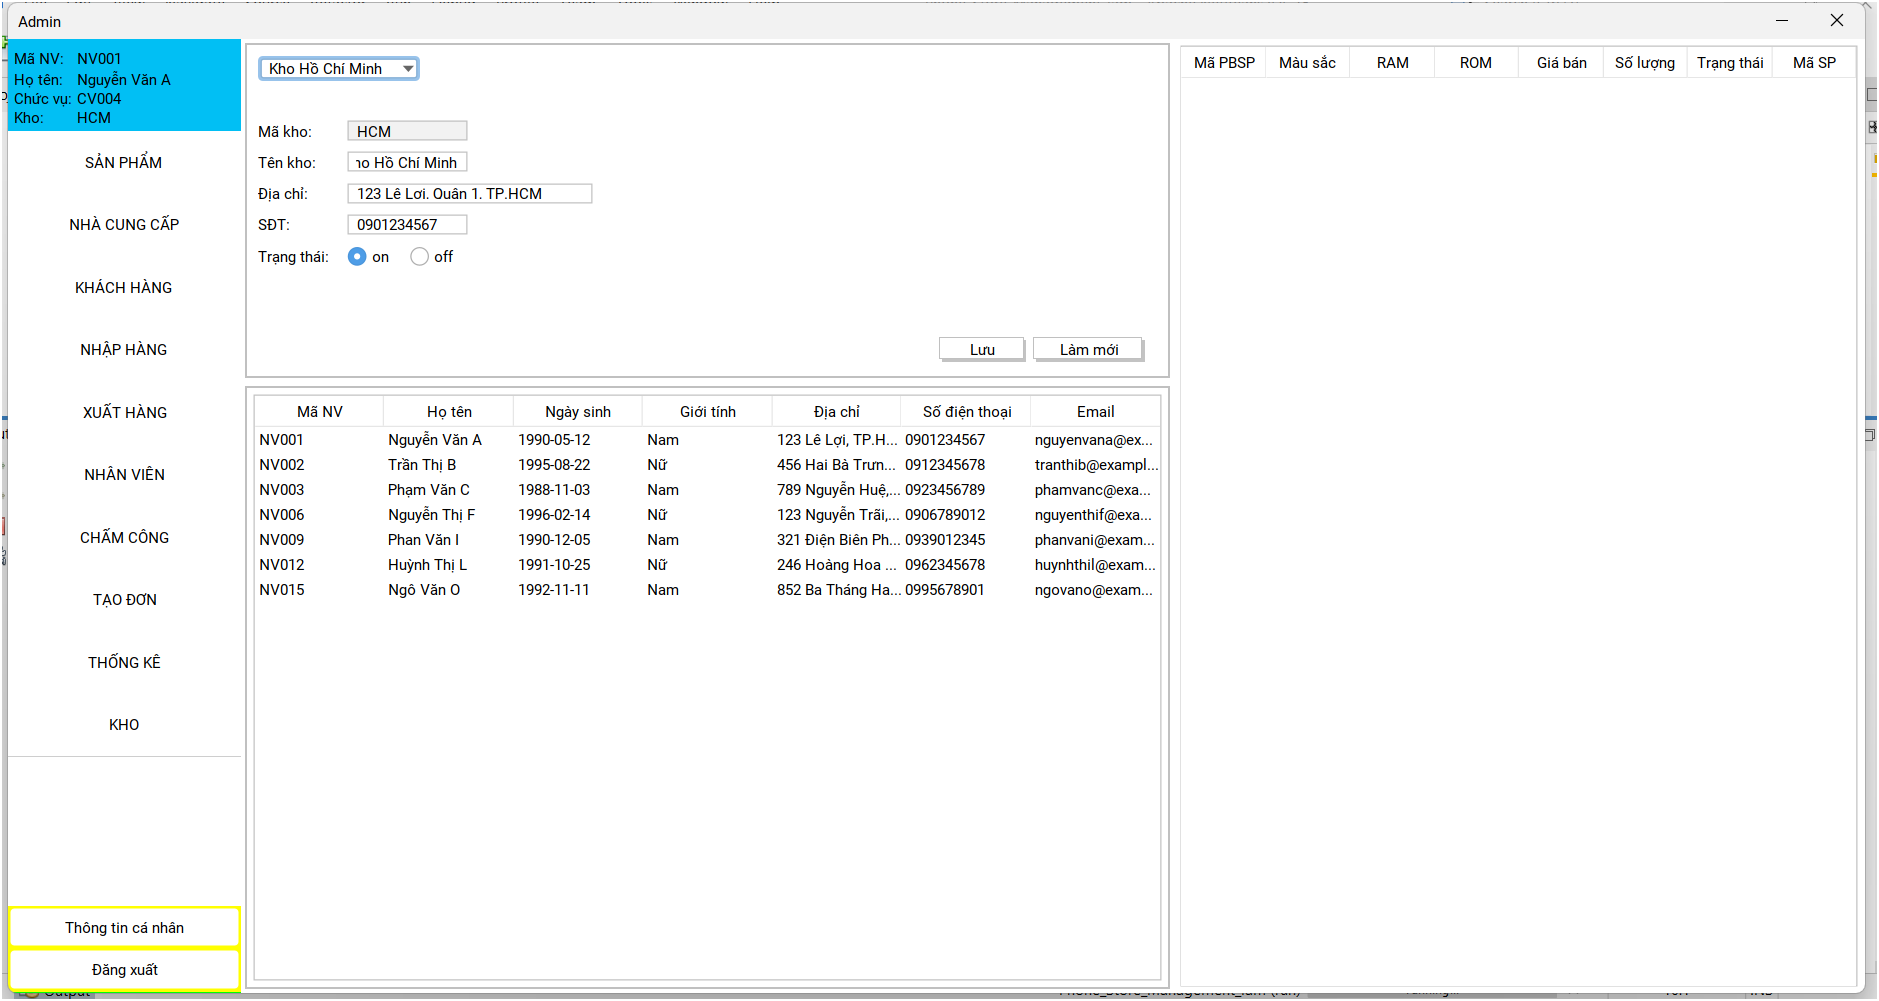
\includegraphics[width=0.8\linewidth]{image/Bao-cao-HTTTDN/giaodien-kho.png}
    \caption{Giao diện kho.}
    \label{fig:image/Bao-cao-HTTTDN/giaodien-kho}
\end{figure}
\begin{figure}[H]
    \centering
    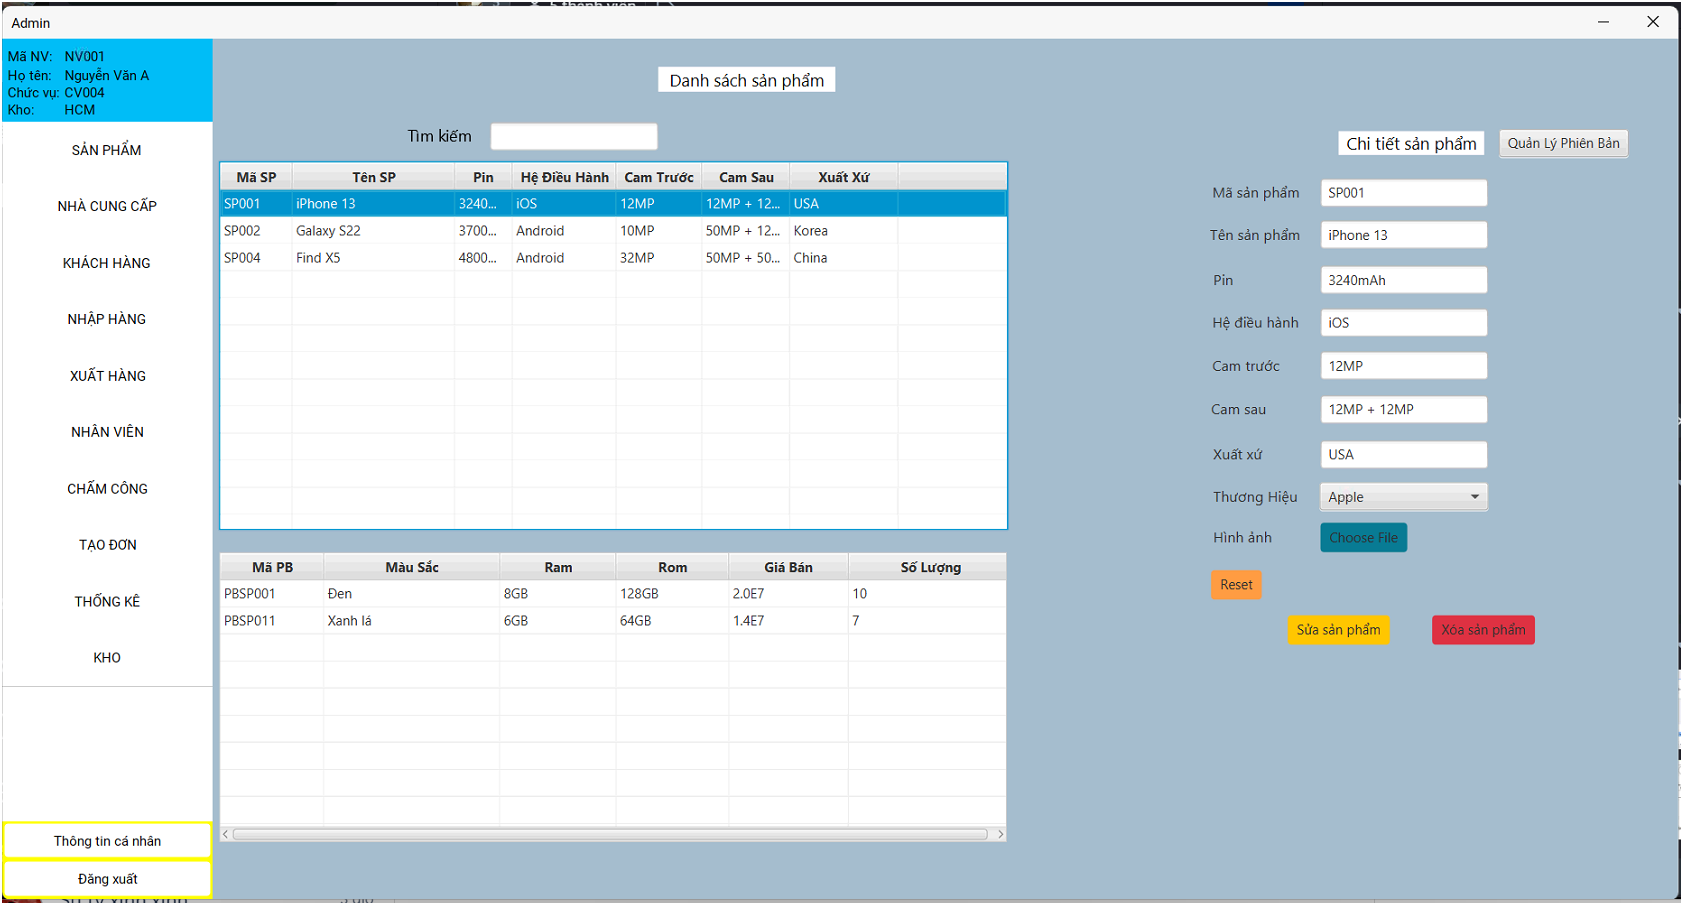
\includegraphics[width=0.8\linewidth]{image/Bao-cao-HTTTDN/giaodien-sanpham.png}
    \caption{Giao diện sản phẩm}
    \label{fig:image/Bao-cao-HTTTDN/giaodien-sanpham}
\end{figure}
\begin{figure}[H]
    \centering
    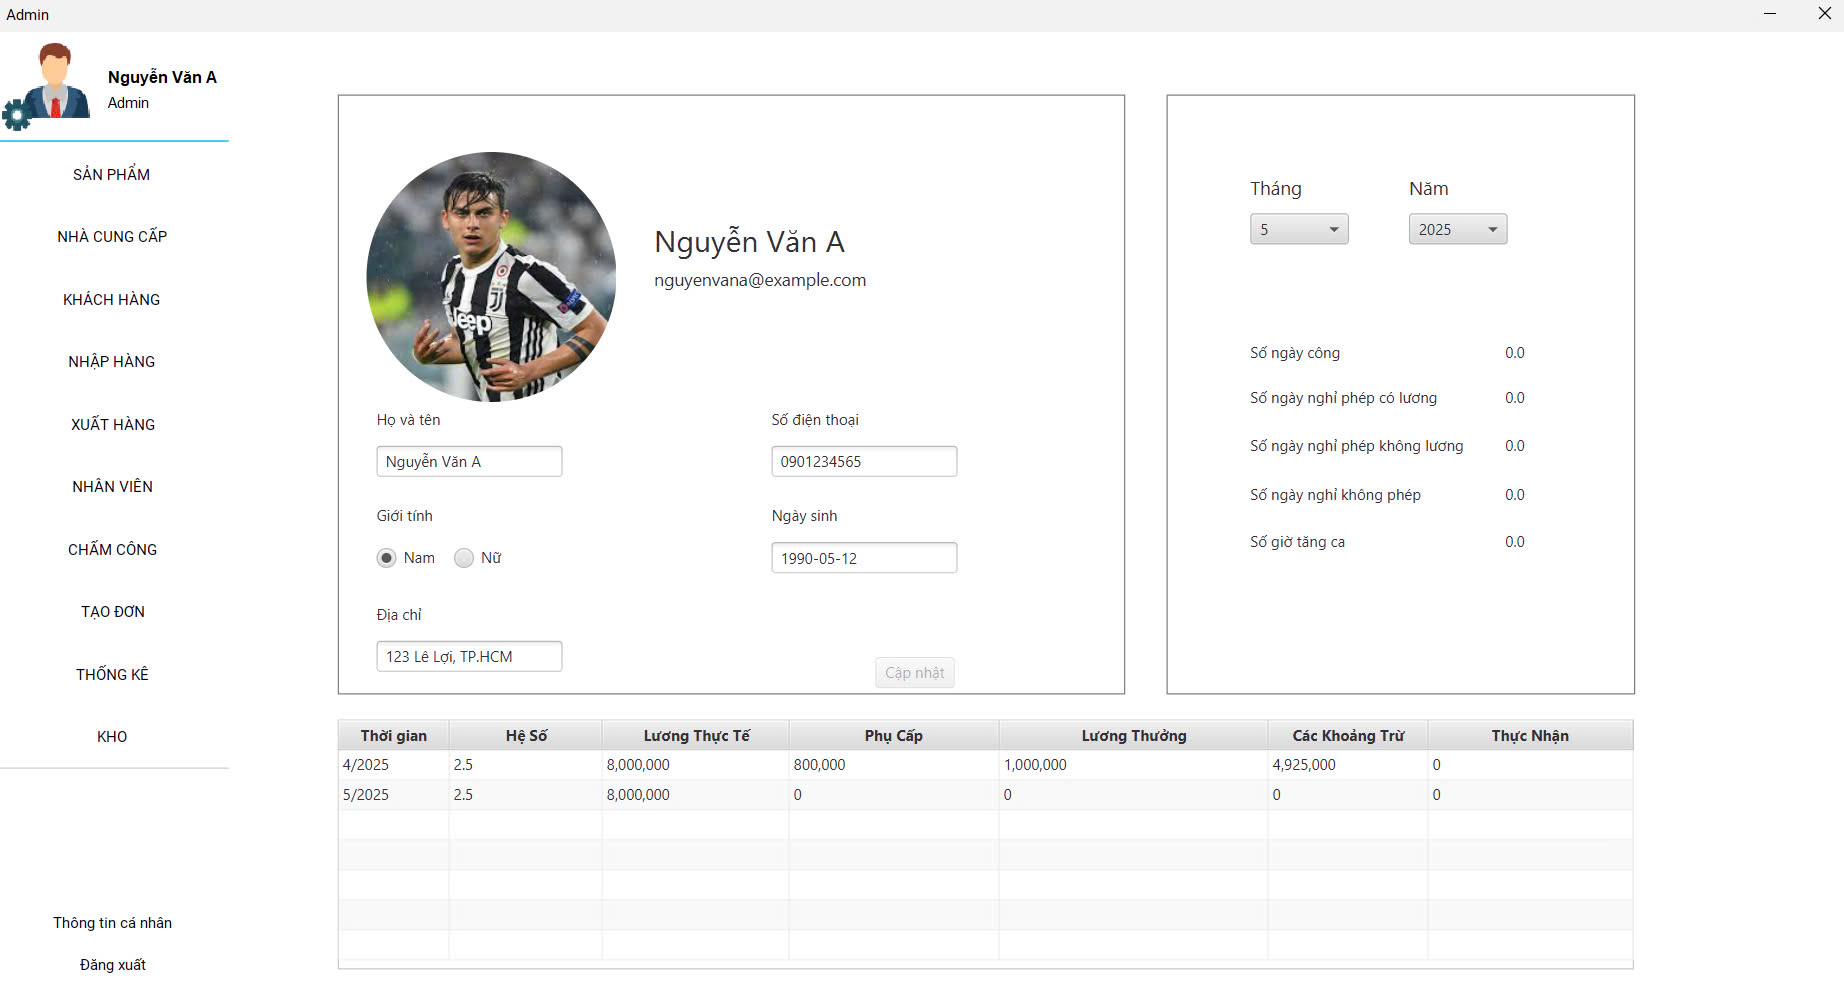
\includegraphics[width=0.8\linewidth]{image/Bao-cao-HTTTDN/giaodien-thongtincanhan.jpg}
    \caption{Giao diện thông tin cá nhân.}
    \label{fig:image/Bao-cao-HTTTDN/giaodien-thongtincanhan}
\end{figure}
\begin{figure}[H]
    \centering
    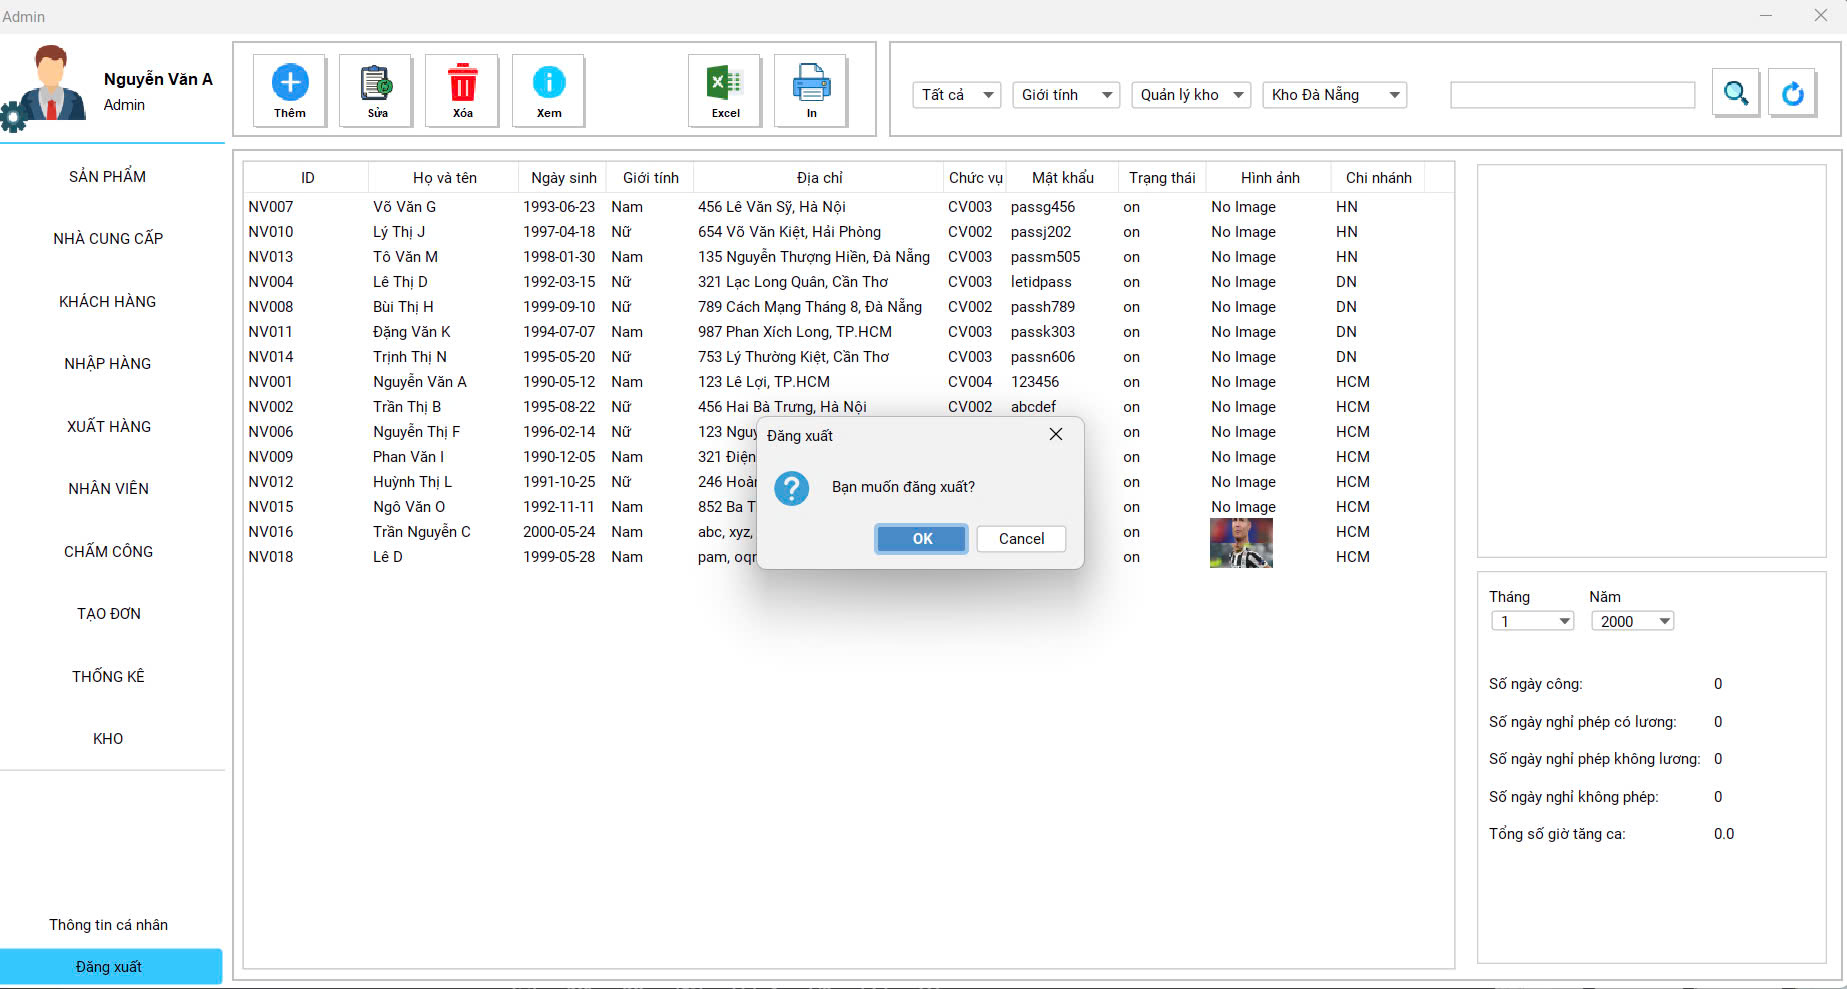
\includegraphics[width=0.8\linewidth]{image/Bao-cao-HTTTDN/giaodien-dangxuat.jpg}
    \caption{Giao diện đăng xuất.}
    \label{fig:image/Bao-cao-HTTTDN/giaodien-dangxuat.jpg}
\end{figure}
\section{Thiết kế các phân mảnh}
\begin{figure}[H]
    \centering
    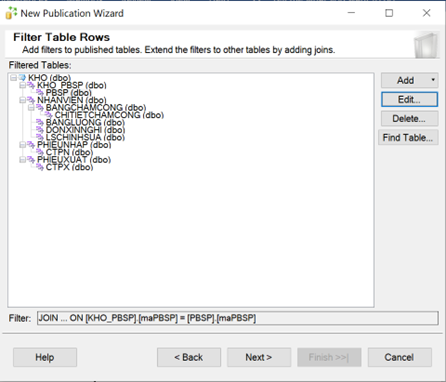
\includegraphics[width=0.8\linewidth]{image/Bao-cao-HTTTDN/17.png}
    \caption{Bảng phân mảnh.}
    \label{fig:image/Bao-cao-HTTTDN/17}
\end{figure}
\begin{minipage}[t]{\linewidth}
    \textbf{Lược đồ phân mảnh:}
    \begin{itemize}[label={}, leftmargin=1.5em]
        \item KHO (Phân mảnh chính/nguyên thuỷ) (Theo Kho\_HN, Kho\_DN, Kho\_HCM)
              \begin{itemize}[label=+, leftmargin=1.5em]
                  \item KHO\_PBSP (Phân mảnh ngang dẫn xuất theo KHO)
                  \item PHIEUNHAP (Phân mảnh ngang dẫn xuất theo KHO)
                        \begin{itemize}[label=+, leftmargin=1.5em]
                            \item CTPN (Phân mảnh ngang dẫn xuất theo PHIEUNHAP)
                        \end{itemize}
                  \item NHANVIEN (Phân mảnh ngang dẫn xuất theo KHO)
                        \begin{itemize}[label=+, leftmargin=1.5em]
                            \item BANGLUONG (Phân mảnh ngang dẫn xuất theo NHANVIEN)
                            \item BANGCHAMCONG (Phân mảnh ngang dẫn xuất theo \newline NHANVIEN)
                                  \begin{itemize}[label=+, leftmargin=1.5em]
                                      \item CHITIETCHAMCONG (Phân mảnh ngang dẫn xuất theo BANGCHAMCONG)
                                  \end{itemize}
                            \item DONXINNGHI (Phân mảnh ngang dẫn xuất theo NHANVIEN)
                            \item LSCHINHSUA (Phân mảnh ngang dẫn xuất theo NHANVIEN)
                        \end{itemize}
                  \item PHIEUXUAT (Phân mảnh ngang dẫn xuất theo KHO)
                  \begin{itemize}[label=+, leftmargin=1.5em]
                    \item CTPX (Phân mảnh ngang dẫn xuất theo PHIEUXUAT)
                  \end{itemize}
              \end{itemize}
        \item THUONGHIEU, SANPHAM, CHUCVU, KHACHHANG, PBSP,\newline NHACUNGCAP: nhân bản (do các site đều như nhau)
    \end{itemize}


\end{minipage}
\chapter{CÀI ĐẶT, BẢO TRÌ HỆ~THỐNG THÔNG~TIN VÀ HƯỚNG~DẪN SỬ DỤNG HỆ THỐNG}
\section{Cài đặt và bảo trì}
\subsection{Cài đặt môi trường phân tán}
\begin{enumerate}[label=B\arabic*:]
    \item Tạo publication trong Replication trên SQL Server Management Studio \newline
          \begin{figure}[H]
              \centering
              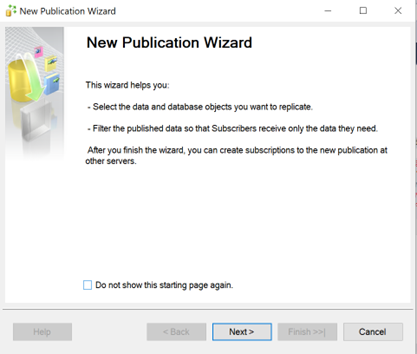
\includegraphics[width=0.8\linewidth]{image/Bao-cao-HTTTDN/1.png}
          \end{figure}
    \item Chọn Next \newline
          \begin{figure}[H]
              \centering
              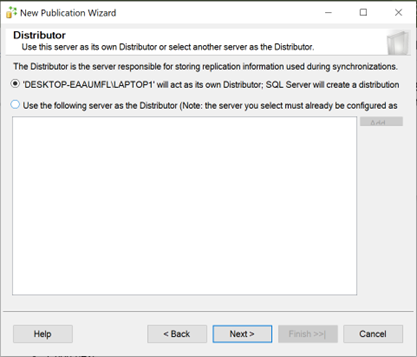
\includegraphics[width=0.8\linewidth]{image/Bao-cao-HTTTDN/2.png}
          \end{figure}
    \item Chọn Next \newline
          \begin{figure}[H]
              \centering
              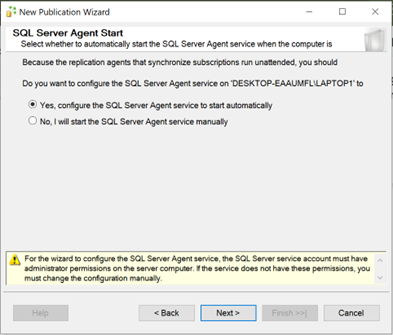
\includegraphics[width=0.45\linewidth]{image/Bao-cao-HTTTDN/3.png} \hfill
              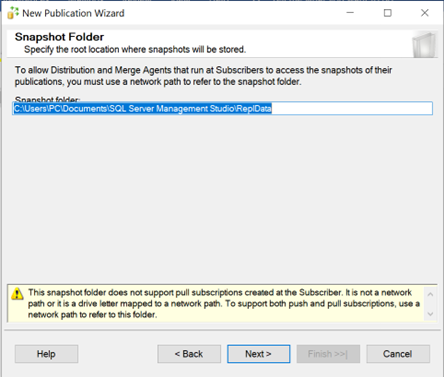
\includegraphics[width=0.45\linewidth]{image/Bao-cao-HTTTDN/4.png} \\
              \vspace{2mm}
              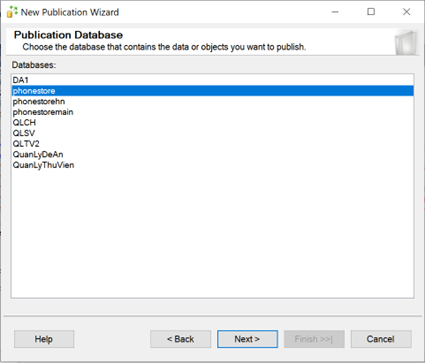
\includegraphics[width=0.45\linewidth]{image/Bao-cao-HTTTDN/5.png} \hfill
              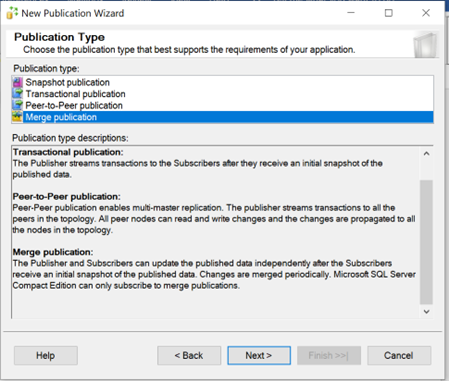
\includegraphics[width=0.45\linewidth]{image/Bao-cao-HTTTDN/6.png} \\
              \vspace{2mm}
              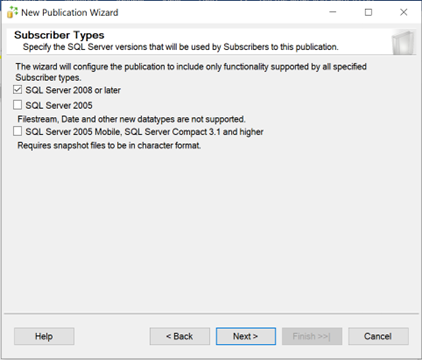
\includegraphics[width=0.45\linewidth]{image/Bao-cao-HTTTDN/7.png} \hfill
              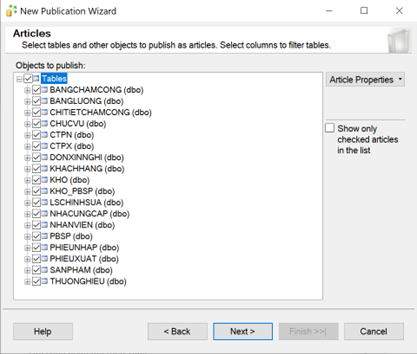
\includegraphics[width=0.45\linewidth]{image/Bao-cao-HTTTDN/8.png} \\
          \end{figure}

          \begin{figure}[H]
              \centering
              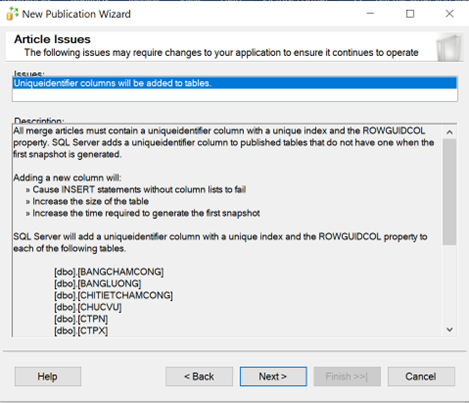
\includegraphics[width=0.45\linewidth]{image/Bao-cao-HTTTDN/9.png} \hfill
              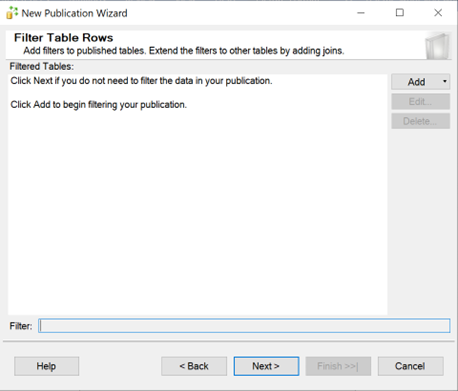
\includegraphics[width=0.45\linewidth]{image/Bao-cao-HTTTDN/10.png} \\
              \vspace{2mm}
              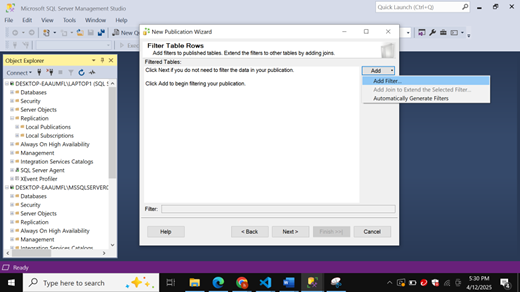
\includegraphics[width=0.45\linewidth]{image/Bao-cao-HTTTDN/11.png} \hfill
              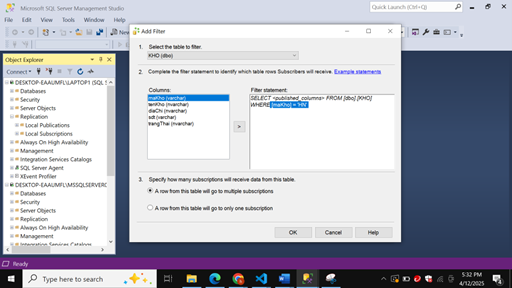
\includegraphics[width=0.45\linewidth]{image/Bao-cao-HTTTDN/12.png} \\
              \vspace{2mm}
              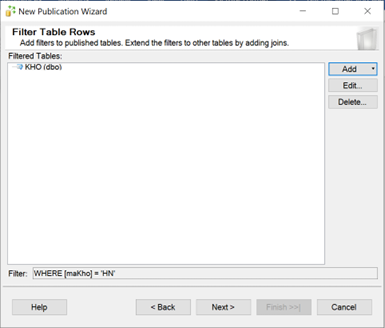
\includegraphics[width=0.45\linewidth]{image/Bao-cao-HTTTDN/13.png} \hfill
              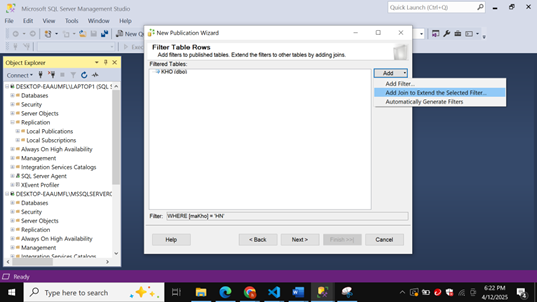
\includegraphics[width=0.45\linewidth]{image/Bao-cao-HTTTDN/14.png} \\
          \end{figure}

          \begin{figure}[H]
              \centering
              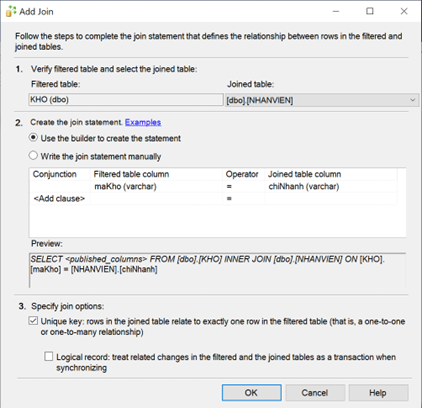
\includegraphics[width=0.45\linewidth]{image/Bao-cao-HTTTDN/15.png} \hfill
              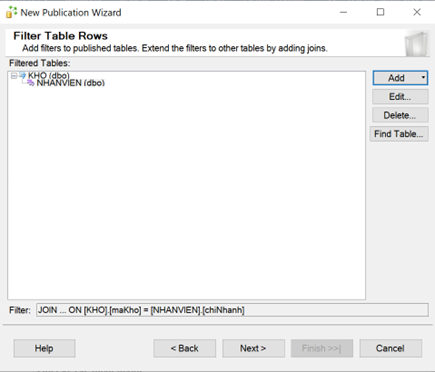
\includegraphics[width=0.45\linewidth]{image/Bao-cao-HTTTDN/16.png} \\
              \vspace{2mm}
              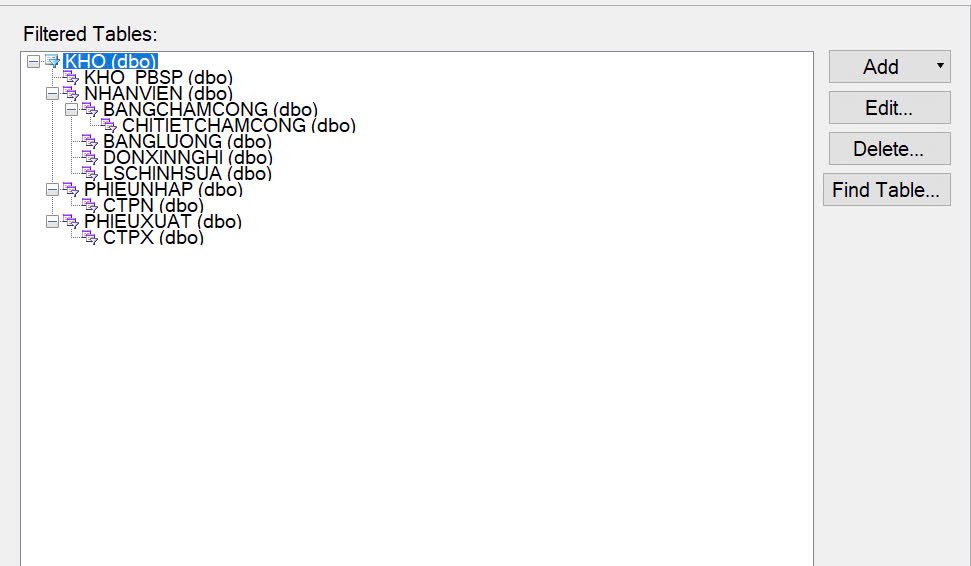
\includegraphics[width=0.45\linewidth]{image/Bao-cao-HTTTDN/21.jpg} \hfill
              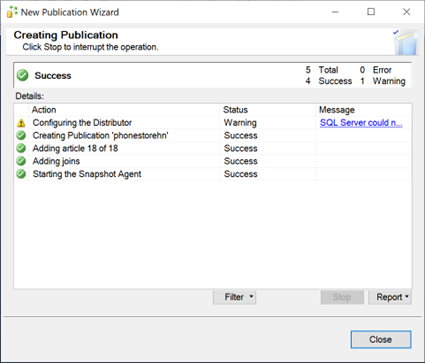
\includegraphics[width=0.45\linewidth]{image/Bao-cao-HTTTDN/18.png} \\
              \vspace{2mm}
              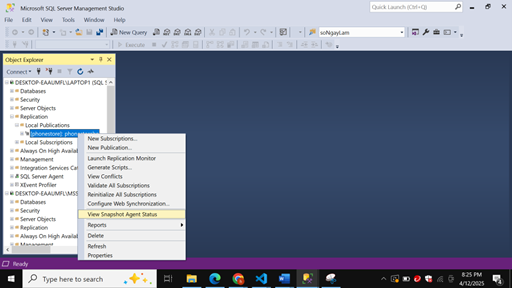
\includegraphics[width=0.6\linewidth]{image/Bao-cao-HTTTDN/19.png}
          \end{figure}

    \item Tạo Subsection để phân tán publication \newline
          \begin{figure}[H]
              \centering
              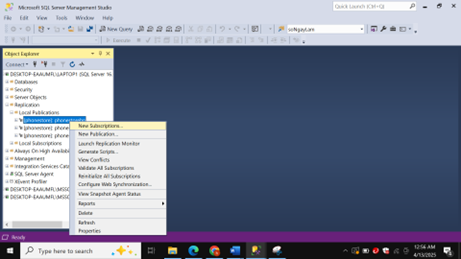
\includegraphics[width=0.45\linewidth]{image/Bao-cao-HTTTDN/22.png} \hfill
              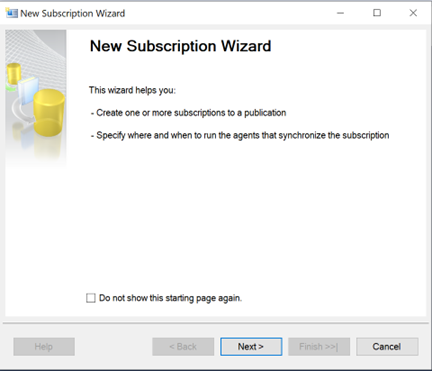
\includegraphics[width=0.45\linewidth]{image/Bao-cao-HTTTDN/23.png} \\
              \vspace{2mm}
              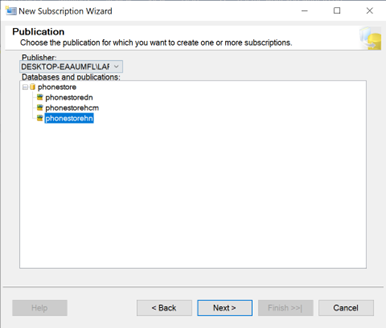
\includegraphics[width=0.45\linewidth]{image/Bao-cao-HTTTDN/24.png} \hfill
              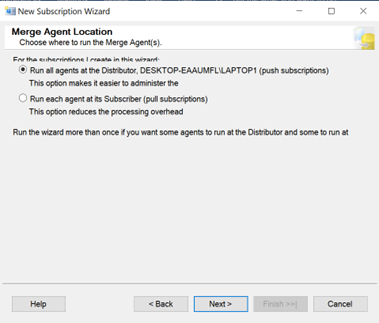
\includegraphics[width=0.45\linewidth]{image/Bao-cao-HTTTDN/25.png} \\
              \vspace{2mm}
              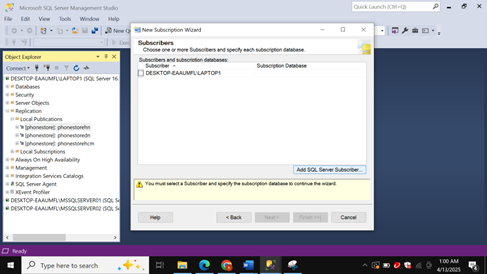
\includegraphics[width=0.45\linewidth]{image/Bao-cao-HTTTDN/26.png} \\
          \end{figure}
    \item Chọn Subscriber (server sẽ chứa dữ liệu phân tán publication \\ phonestorehn). Có thể chọn server khác để chứa dữ liệu phân tán này Add~SQL~server~Subscriber. \newline
          \begin{figure}[H]
              \centering
              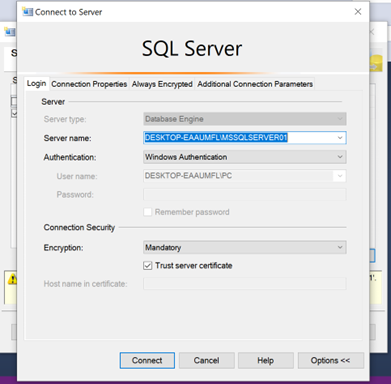
\includegraphics[width=0.45\linewidth]{image/Bao-cao-HTTTDN/27.png} \hfill
              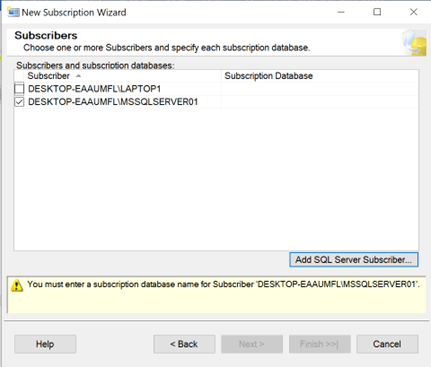
\includegraphics[width=0.45\linewidth]{image/Bao-cao-HTTTDN/28.png} \\
              \vspace{2mm}
              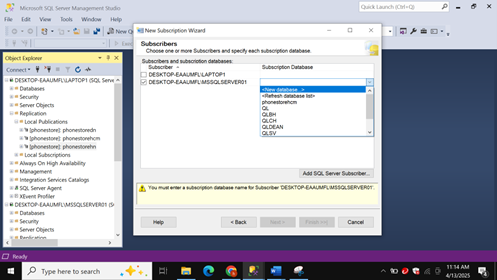
\includegraphics[width=0.45\linewidth]{image/Bao-cao-HTTTDN/29.png} \hfill
              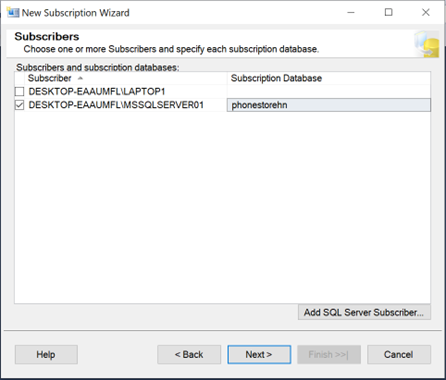
\includegraphics[width=0.45\linewidth]{image/Bao-cao-HTTTDN/30.png} \\
              \vspace{2mm}
              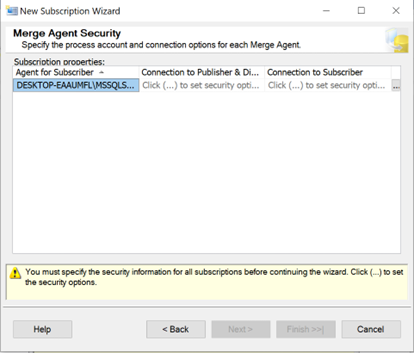
\includegraphics[width=0.45\linewidth]{image/Bao-cao-HTTTDN/31.png} \hfill
              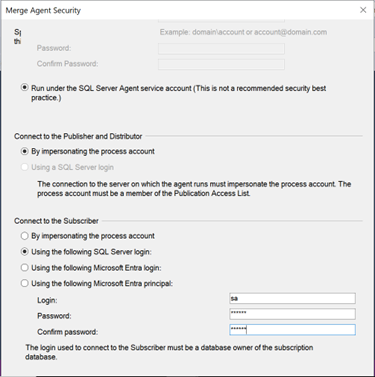
\includegraphics[width=0.45\linewidth]{image/Bao-cao-HTTTDN/32.png} \\
          \end{figure}
    \item Tài khoản login vào Subscriber (MSSQLSERVER01) \newline
          \begin{figure}[H]
              \centering
              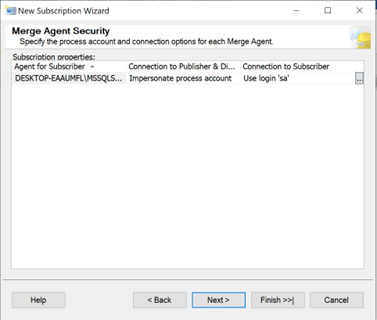
\includegraphics[width=0.45\linewidth]{image/Bao-cao-HTTTDN/33.png} \hfill
              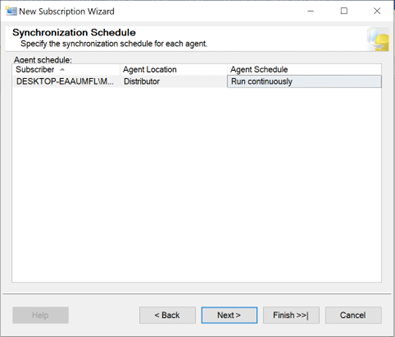
\includegraphics[width=0.45\linewidth]{image/Bao-cao-HTTTDN/34.png} \\
          \end{figure}
    \item Chọn Run continuously \newline
          \begin{figure}[H]
              \centering
              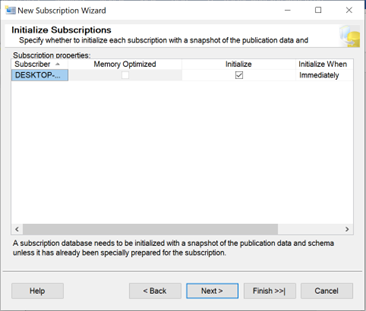
\includegraphics[width=0.45\linewidth]{image/Bao-cao-HTTTDN/35.png} \hfill
              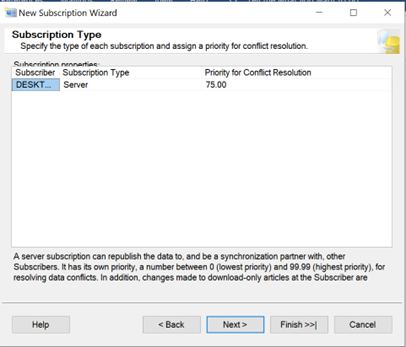
\includegraphics[width=0.45\linewidth]{image/Bao-cao-HTTTDN/36.png} \\
              \vspace{2mm}
              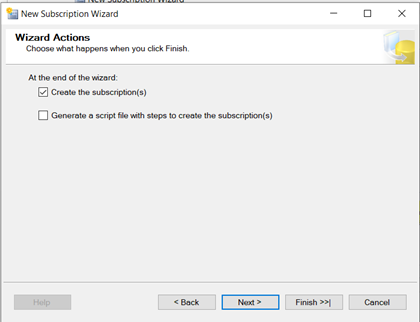
\includegraphics[width=0.45\linewidth]{image/Bao-cao-HTTTDN/37.png} \hfill
              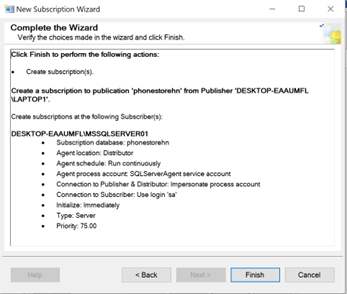
\includegraphics[width=0.45\linewidth]{image/Bao-cao-HTTTDN/38.png} \\
              \vspace{2mm}
              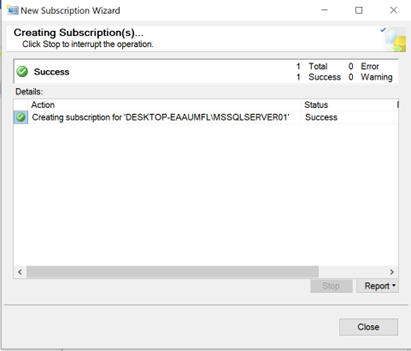
\includegraphics[width=0.45\linewidth]{image/Bao-cao-HTTTDN/39.png} \hfill
              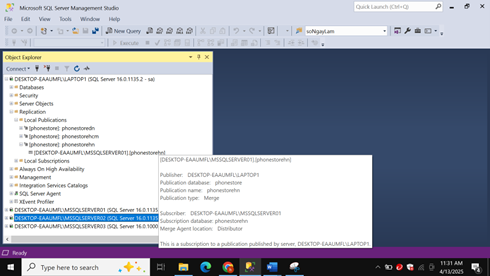
\includegraphics[width=0.45\linewidth]{image/Bao-cao-HTTTDN/40.png} \\
          \end{figure}

          \begin{itemize}
              \item Distributor và Publisher là .\textbackslash LAPTOP1
                    \begin{itemize}
                        \item Database gốc (toàn cục): phonestore
                        \item Publication: phonestorehn (dữ liệu phân tán của KHO1)
                    \end{itemize}
              \item Subscriber: .\textbackslash MSSQLSERVER01
                    \begin{itemize}
                        \item Database chứa dữ liệu phân tán tương ứng với Publication \newline phonestorehn: phonestore
                        \item Mở server .\textbackslash MSSQLSERVER01, sẽ thấy hình phía dưới sau:
                              \begin{figure}[H]
                                  \centering
                                  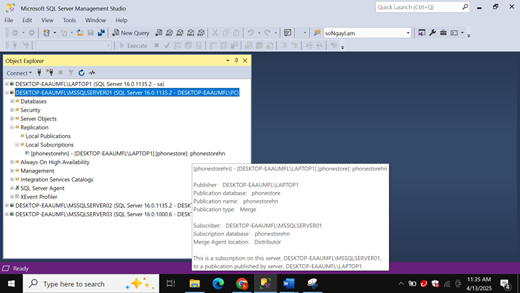
\includegraphics[width=0.5\linewidth]{image/Bao-cao-HTTTDN/41.png}
                                  \vspace{2mm}
                                  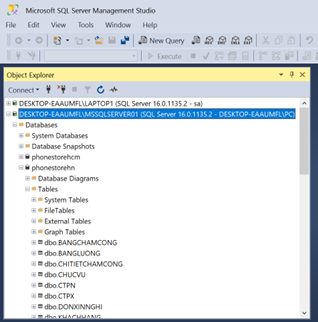
\includegraphics[width=0.5\linewidth]{image/Bao-cao-HTTTDN/42.png} \\
                              \end{figure}
                        \item Và database phonestorehn sẽ có các table ứng với các phân mảnh trong publication phonestore
                    \end{itemize}
          \end{itemize}
    \item Tạo link server
          \begin{itemize}
              \item Quy tắc:
                    \begin{itemize}
                        \item Tên các csdl ở các server subscriber phải giống nhau
                        \item Tên link server phải giống nhau
                    \end{itemize}
              \item Các bước thực hiện sau:
                    \begin{enumerate}[label=B8.\arabic*:]
                        \item Tạo remotelogin tên "HTKN" (Hỗ trợ kết nối - dùng cho phép connect) ở cả 4 server
                        \item Phân quyền account "HTKN" cho thấy database "phonestore"
                        \item Tạo linked server như sau:
                              \begin{itemize}[label=+]
                                  \item Trên server gốc tạo linked server LINK1, LINK2, LINK3 lần~lượt trỏ đến server 1, server 2, server 3
                                  \item Trên server 1 tạo linked server LINK0, LINK2, LINK3 lần lượt trỏ đến server gốc, server 2, server 3
                                  \item Trên server 2 tạo linked server LINK0, LINK1, LINK3 lần lượt trỏ đến server gốc, server 1, server 3
                                  \item Trên server 3 tạo linked server LINK0, LINK1, LINK2 lần lượt trỏ đến server gốc, server 1, server 2
                              \end{itemize}

                              \begin{figure}[H]
                                  \centering
                                  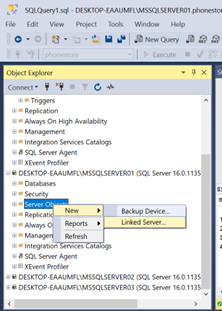
\includegraphics[width=0.4\linewidth]{image/Bao-cao-HTTTDN/43.png} \hfill
                                  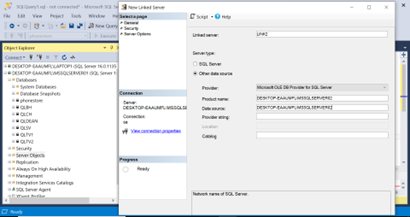
\includegraphics[width=0.45\linewidth]{image/Bao-cao-HTTTDN/44.png} \\
                                  \vspace{2mm}
                                  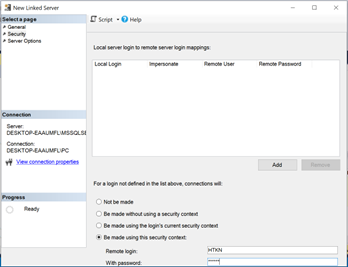
\includegraphics[width=0.45\linewidth]{image/Bao-cao-HTTTDN/45.png} \hfill
                                  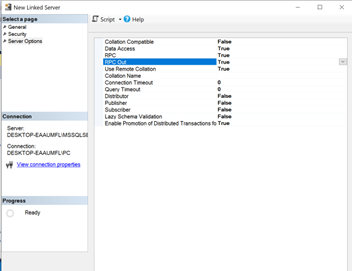
\includegraphics[width=0.45\linewidth]{image/Bao-cao-HTTTDN/46.png} \\
                              \end{figure}

                              \begin{itemize}
                                  \item RPC (Remote Procedure Call): Cho phép máy chủ SQL hiện tại có thể chạy thủ tục lưu trữ (Stored Procedures) từ linked server (máy chủ liên kết). Tức là bạn có thể gọi thủ tục từ server khác như: \newline \texttt{EXEC [LinkedServerName].DatabaseName.dbo.StoredProcedureName}
                                  \item RPC Out: Cho phép linked server gọi Stored Procedures trên chính máy chủ hiện tại
                                  \item Nghĩa là nếu máy chủ A liên kết đến B và RPC Out = True, thì B có thể gọi thủ tục trên A
                              \end{itemize}

                              \textbf{Chú ý:} Tạo linked server LINK0 tại server gốc để tránh bị báo lỗi khi truy vấn. \newline
                              \begin{figure}[H]
                                  \centering
                                  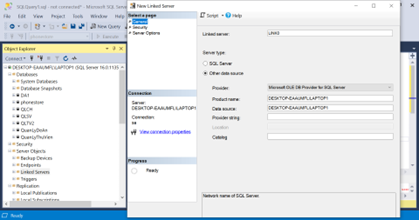
\includegraphics[width=0.5\linewidth]{image/Bao-cao-HTTTDN/47.png} \\
                                  \vspace{2mm}
                                  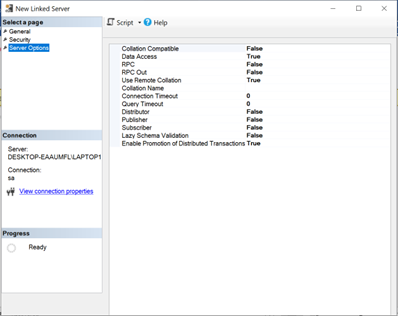
\includegraphics[width=0.5\linewidth]{image/Bao-cao-HTTTDN/48.png}
                              \end{figure}
                    \end{enumerate}
          \end{itemize}
    \item Thực hiện đẩy một Stored Procedure về phân mảnh sau:
          \begin{enumerate}[label=B9.\arabic*:]
              \item Vào replication chọn phân mảnh muốn đẩy xuống
              \item Nhấn chuột phải chọn Properties
              \item Chọn Articles -> bỏ dấu tích "show only checked articles of the list
              \item Đánh dấu các stored procedure muốn sử dụng tại phân mảnh đó
              \item Nhấn OK để kết thúc
              \item Chuột phải lại vào phân mảnh chọn "view snapshot agent status" \textrightarrow{} start để nó đẩy xuống phân mảnh
          \end{enumerate}
\end{enumerate}
\subsection{Bảo trì hệ thống và xử lý lỗi}
\quad Xử lý lỗi hay thường gặp:
\begin{figure}[H]
    \centering
    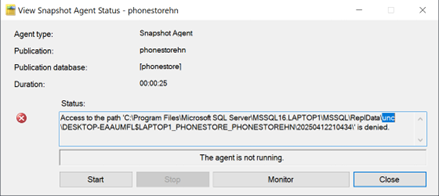
\includegraphics[width=0.8\linewidth]{image/Bao-cao-HTTTDN/20-loi.png}   \\
\end{figure}
\begin{minipage}[t]{\linewidth}
    \begin{enumerate}[label=B\arabic*:]
        \item Cấp quyền cho thư mục ReplData:
              \begin{itemize}
                  \item Mở File Explorer và đi tới đường dẫn: \texttt{C:\textbackslash Program Files\textbackslash Microsoft SQL Server\textbackslash MSSQL16.LAPTOP1\textbackslash MSSQL\textbackslash ReplData}
                  \item Chuột phải vào thư mục ReplData \textrightarrow{} chọn Properties
                  \item Vào tab Security \textrightarrow{} nhấn Edit
                  \item Nhấn Add, rồi nhập: \texttt{NT SERVICE\textbackslash SQLSERVERAGENT} hoặc nếu bạn dùng SQL Server Agent bằng tài khoản khác (như NETWORK \\ SERVICE hay một tài khoản domain), thì nhập đúng tài khoản đó
                  \item Sau khi thêm, chọn Allow quyền Full Control hoặc ít nhất là Modify, Read \& Execute, Write
                  \item Nhấn OK để lưu và thoát
              \end{itemize}
        \item Kiểm tra tài khoản đang chạy SQL Server Agent
              \begin{itemize}
                  \item Mở SQL Server Configuration Manager
                  \item Chọn SQL Server Services
                  \item Kiểm tra dịch vụ: SQL Server (<instance\_name>), SQL Server Agent (<instance\_name>)
                  \item Xem cột Log On As để biết tài khoản nào đang chạy
              \end{itemize}
        \item Khởi động lại SQL Server Agent và thử lại
              \begin{itemize}
                  \item Mở SQL Server Management Studio (SSMS)
                  \item Trong Object Explorer, chuột phải vào SQL Server Agent \textrightarrow{} chọn Start (nếu chưa chạy)
                  \item Quay lại phần Replication → click phải vào Publication \textrightarrow{} chọn View Snapshot Agent Status \textrightarrow{} bấm Start lại
              \end{itemize}
    \end{enumerate}
\end{minipage}
\subsection{Sao lưu và phục hồi dữ liệu}
\quad Trong quá trình vận hành hệ thống, có thể xảy ra lỗi ngoài ý muốn dẫn đến hư tổn dữ liệu. Vì vậy ta cần có phương án back up dữ liệu, dưới đây là một trong những cách back up dữ liệu cho hệ thống.

    \begin{enumerate}[label=B\arabic*:]
        \item Mở SQL Server Management Studio
        \item Click chuột phải vào database phonestore \textrightarrow{} chọn Tasks \textrightarrow{} chọn Back~Up
        \begin{figure}[H]
            \centering
            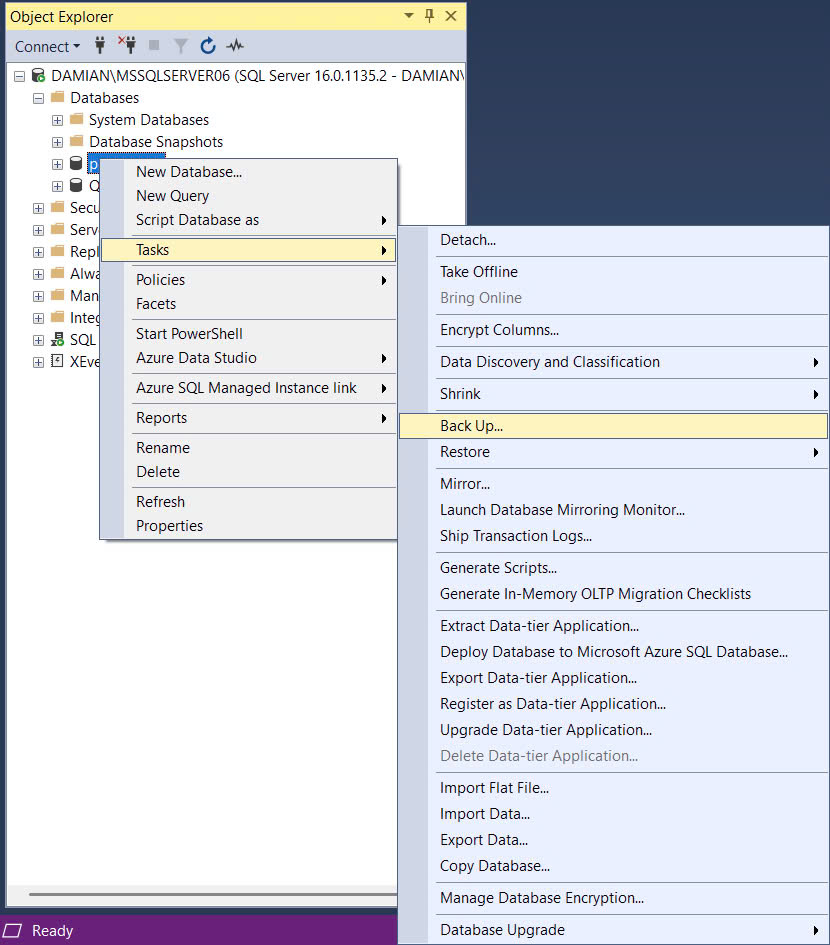
\includegraphics[width=0.6\linewidth]{image/Bao-cao-HTTTDN/1-1.jpg}
        \end{figure}
        \item Chọn Type là Full để backup toàn bộ
        \begin{figure}[H]
            \centering
            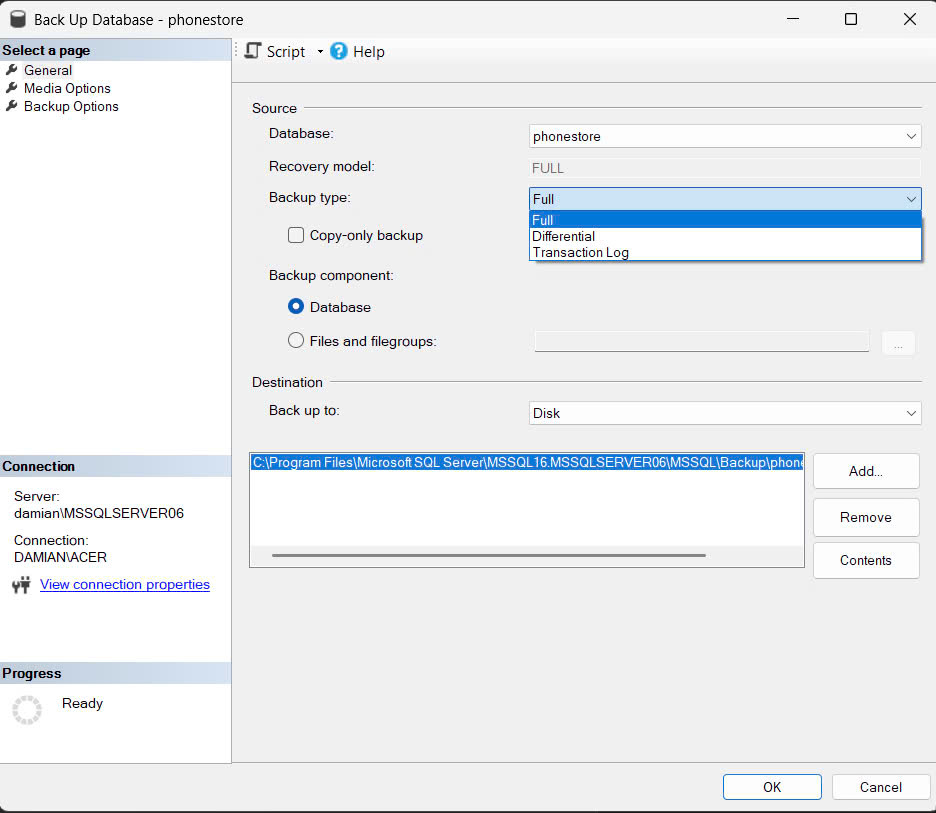
\includegraphics[width=0.6\linewidth]{image/Bao-cao-HTTTDN/1-2.jpg}
        \end{figure}
        \item Chọn Back up to: Disk để lưu back up vào ổ đĩa
        \begin{figure}[H]
            \centering
            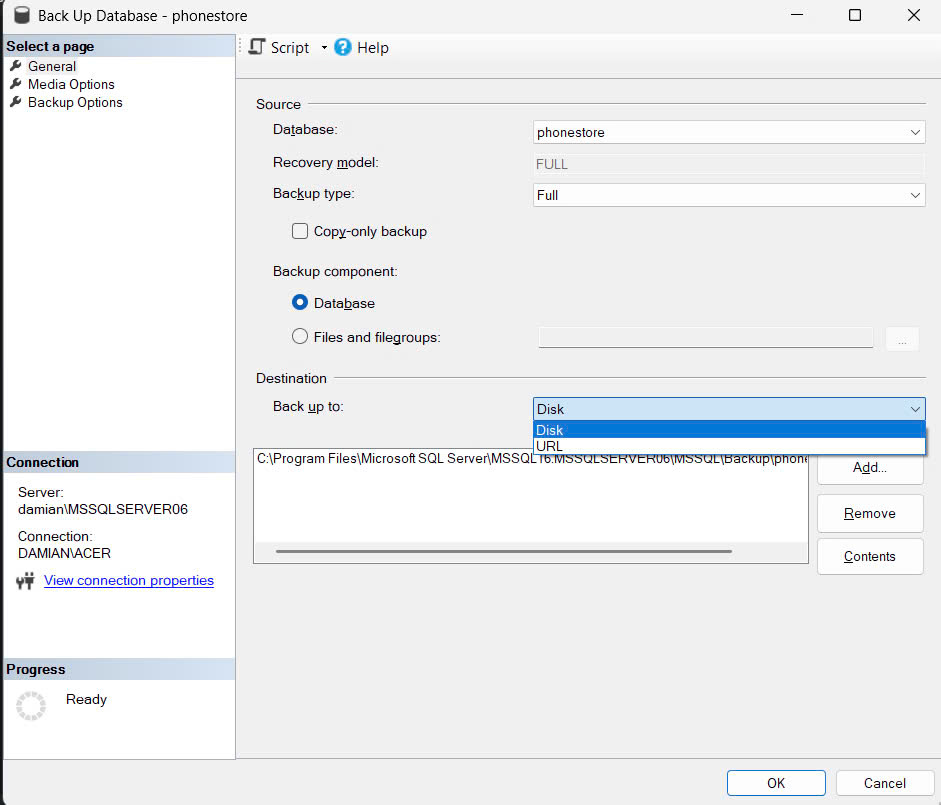
\includegraphics[width=0.6\linewidth]{image/Bao-cao-HTTTDN/1-3.jpg}
        \end{figure}
        \item Chọn đường dẫn
        \begin{figure}[H]
            \centering
            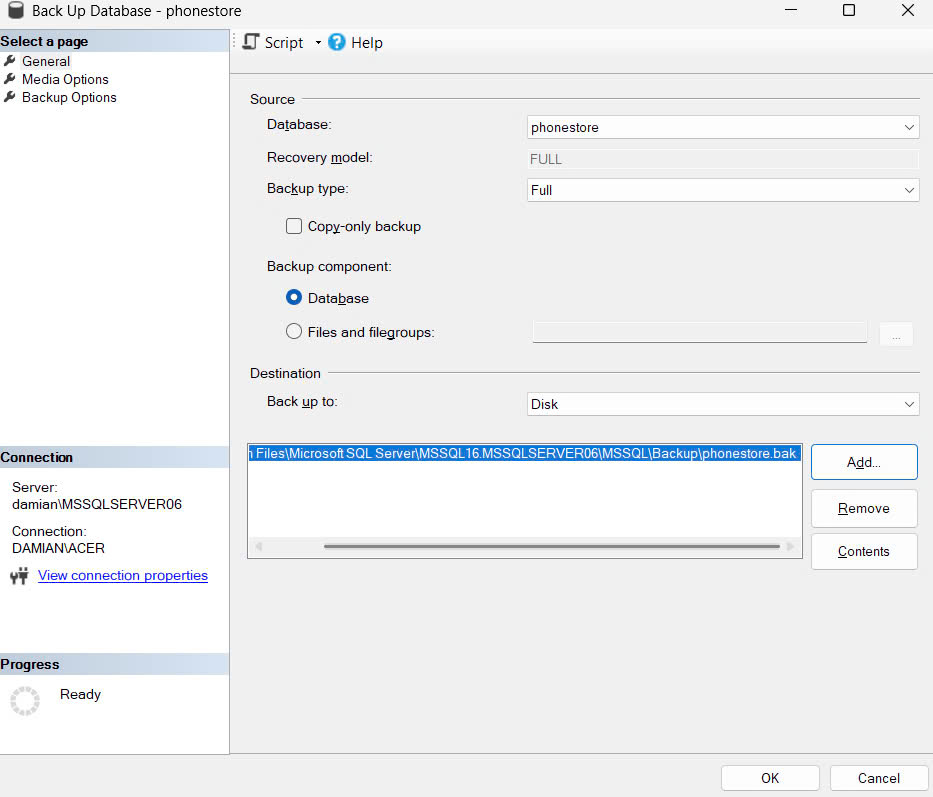
\includegraphics[width=0.6\linewidth]{image/Bao-cao-HTTTDN/1-4.jpg}
        \end{figure}
        \item Chọn OK để bắt đầu quá trình backup. Khi hoàn thành, hệ thống sẽ thông báo "The backup of database completed successfully."
        \begin{figure}[H]
            \centering
            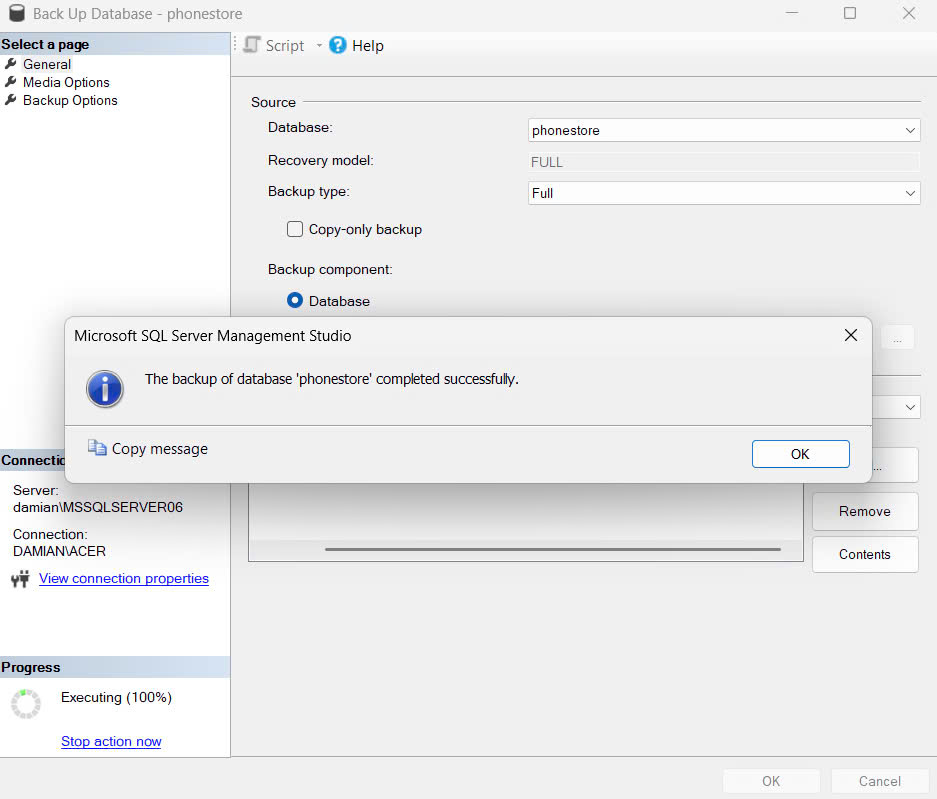
\includegraphics[width=0.6\linewidth]{image/Bao-cao-HTTTDN/1-5.jpg}
        \end{figure}
        \item Kết quả: File back up đã được tạo thành công và nằm đúng thư mục ta đã định sẵn
        \begin{figure}[H]
            \centering
            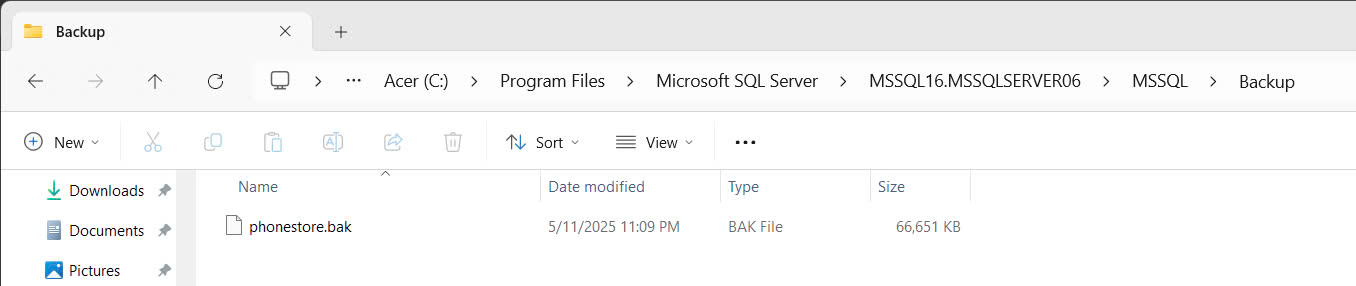
\includegraphics[width=0.8\linewidth]{image/Bao-cao-HTTTDN/1-6.jpg}
        \end{figure}
    \end{enumerate}
    \textbf{Lưu ý:} Để phục hồi dữ liệu, bạn chỉ cần click chuột phải vào database phonestore \textrightarrow{} chọn Tasks \textrightarrow{} chọn Restore \textrightarrow{} chọn file sao lưu đã tạo ở trên

\section{Hướng dẫn sử dụng hệ thống}
\subsection{Cài đặt môi trường}
\begin{itemize}
    \item Cài đặt Java Development Kit (JDK) 20 trở lên
    \item Cài đặt phần mềm NetBeans IDE (khuyến nghị bản 15 trở lên)
    \item Cài đặt SQL Server Management Studio 20 trở lên
\end{itemize}
\subsection{Cấu hình dự án}
\begin{minipage}[t]{\linewidth}
    \begin{itemize}
        \item Clone hoặc tải source code từ link: \url{https://github.com/Ttuandatt/Phone_Store_Management}
        \item Mở NetBeans, chọn File > Open Project, rồi chọn thư mục dự án Phone\_Store\_Management
        \item Đảm bảo các thư viện (lib) đã được add vào project. Nếu thiếu, vào \\ Properties > Libraries > Add JAR/Folder và thêm các file trong thư mục jars
    \end{itemize}
\end{minipage}

\subsection{Thiết lập CSDL}
\begin{minipage}[t]{\linewidth}
    \begin{itemize}
        \item Mở SQL Server Management Studio 20 và connection tới SQL Server \newline Services.
        \item Truy cập vào Databases \textrightarrow{} chọn New Database, tạo database mới tên phonestore (hoặc tên cùng với tên kết nối)
        \item Import file SQL:
              \begin{itemize}
                  \item Click chuột phải vào database vừa tạo -> chọn New query
                  \item Mở file phonestore.sql bằng Notepad hoặc bất kỳ trình soạn thảo nào
                  \item Copy toàn bộ nội dung và paste vào cửa sổ New Query trong SSMS
                  \item Bấm nút Execute để chạy câu lệnh, tạo các bảng và dữ liệu mẫu
              \end{itemize}
        \item Kiểm tra: Expand database \textrightarrow{} Expand Tables \textrightarrow{} Xem danh sách bảng đã được tạo thành công
    \end{itemize}
\end{minipage}
\subsection{Back up dữ liệu}
\begin{enumerate}[label=B\arabic*:]
    \item Kiểm tra thông tin trong file .bak
    \begin{itemize}
        \item Trước tiên, sử dụng lệnh sau để xem các tên logic (logical name) của các file dữ liệu và log có trong bản sao lưu: \newline
        \begin{verbatim}
RESTORE FILELISTONLY 
FROM DISK = 'D:\Backups\phonestore.bak';
        \end{verbatim}
        \item Kết quả sẽ trả về các cột như: LogicalName, PhysicalName,\newline Type (D = Data, L = Log). Ghi lại các tên logic này để sử dụng ở bước tiếp theo.
    \end{itemize}
    \item Phục hồi cơ sở dữ liệu từ file .bak
    \begin{itemize}
        \item Sử dụng lệnh sau để phục hồi dữ liệu. Ví dụ nếu phonestore\_data và phonestore\_log là các tên logic đã thu được từ bước trên: \newline
        \begin{verbatim}
RESTORE DATABASE phonestore
FROM DISK = 'D:\Backups\phonestore.bak'
WITH MOVE 'phonestore_data' TO 'D:\MSSQL\DATA\phonestore.mdf',
    MOVE 'phonestore_log' TO 'D:\MSSQL\DATA\phonestore_log.ldf',
    REPLACE;
        \end{verbatim}
        \item Lưu ý:
        \begin{itemize}
            \item Thay đổi đường dẫn cho phù hợp với hệ thống của bạn.
            \item Tham số REPLACE sẽ ghi đè nếu cơ sở dữ liệu cùng tên đã tồn tại. Nếu không muốn ghi đè, hãy bỏ REPLACE.
        \end{itemize}
    \end{itemize}    
    \item Ghi chú cho hệ thống phân tán (Replication) \newline
    File phonestore.bak thường là bản sao lưu toàn bộ cơ sở dữ liệu gốc trước khi triển khai phân tán. Do đó:
    \begin{itemize}
        \item Nếu bạn muốn tái triển khai hệ thống phân tán, hãy restore file này vào server trung tâm (Publisher) rồi cấu hình lại các publication như KHO\_HN, KHO\_DN, KHO\_HCM.
        \item Nếu bạn muốn restore vào một trong các server con (ví dụ: server3, server4, server5), cần lưu ý:
        \begin{itemize}
            \item File này có thể chứa dữ liệu của toàn bộ hệ thống, không chỉ riêng một mảnh.
            \item Nếu đã có replication, cần kiểm tra kỹ vì restore có thể gây xung đột schema hoặc dữ liệu.
        \end{itemize}
    \end{itemize}
\end{enumerate}

\subsection{Chạy hệ thống}
\begin{itemize}
    \item Bấm Run Project (Shift + F6) trong NetBeans
    \item Giao diện hệ thống chạy: \newline
          \textbf{Ghi chú:} (Các hình ảnh minh họa cho các bước thao tác được trình bày chi tiết trong mục "4.3 Các giao diện của phần mềm") \newline
          \begin{itemize}
              \item Đăng nhập hệ thống
                    \begin{enumerate}[label=B\arabic*:]
                        \item Nhập tài khoản và mật khẩu vào ô tương ứng
                        \item Bấm nút "Đăng nhập" để truy cập
                    \end{enumerate}
              \item Quản lý sản phẩm
                    \begin{enumerate}[label=B\arabic*:]
                        \item Nhấn mục "SẢN PHẨM" trong thanh menu bên trái để mở giao~diện quản lý sản phẩm
                        \item Tìm kiếm sản phẩm cần xem hoặc chỉnh sửa bằng cách nhập từ khóa vào ổ "Tìm kiểm" phía trên bảng danh sách
                        \item Nhấn vào một dòng trong bảng để hiển thị chi tiết thông tin sản~phẩm ở bên phải màn hình
                        \item Thực hiện các thao tác sau tùy theo nhu cầu:
                              \begin{itemize}
                                  \item Sửa sản phảm: Thay đổi các thông tin như tên sản phẩm, pin, hệ~điều hành, camera, xuất xứ, thương hiệu,...
                                  \item Reset: Nhấn nút "Reset" để xóa nội dung đang hiển thị trong khung chi tiết
                                  \item Xóa sản phẩm: Nhấn "Xóa sản phẩm" để xóa sản phẩm đã chọn khỏi hệ thống
                              \end{itemize}
                        \item Quan sát bảng danh sách phiên bản sản phẩm (phía dưới) để xem các biến thể như màu sắc, RAM, ROM, giá bán, số lượng tương ứng với sản phẩm đang được chọn
                    \end{enumerate}
              \item Quản lý nhà cung cấp
                    \begin{enumerate}[label=B\arabic*:]
                        \item Nhấn mục "NHÀ CUNG CẤP" trong thanh menu bên trái để mở giao~diện quản lý nhà cung cấp
                        \item Tìm kiếm nhà cung cấp cần xem hoặc nhấn vào combobox vào ô cần tìm ở phía trên và nhấn icon tìm kiếm
                        \item Thực hiên các thao tác sau tùy chỉnh theo nhu cầu:
                              \begin{itemize}
                                  \item Thêm nhà cung cấp: Khi nhấn nút icon "Thêm" sẽ hiện giao diện nhập các thông tin nhà cung cấp (tên nhà cung cấp, số điện thoại, email, địa chỉ, trạng thái sau đó nhấn nút "Lưu")
                                  \item Sửa nhà cung cấp: Nhấn chọn 1 dòng trong bảng danh sách nhà cung cấp để sửa thông tin cần sửa
                                  \item Xóa nhà cung cấp: Chọn 1 dòng trong danh sách nhà cung cấp để xóa. Hệ thống sẽ xác nhận lại có xóa không sau đó sẽ thực hiện xóa
                                  \item Xem nhà cung cấp: Chọn 1 dòng trong danh sách nhà cung cấp sau đó hệ thống sẽ hiện đầy đủ thông tin nhà cung cấp
                                  \item Xuất file Excel: Khi nhấn nút icon "Excel" thì hệ thống sẽ xuất file excel cho người dùng
                                  \item In file: Khi nhấn nút icon "In" thì hệ thống sẽ in file pdf cho người~dùng
                              \end{itemize}
                    \end{enumerate}
              \item Quản lý khách hàng
                    \begin{enumerate}[label=B\arabic*:]
                        \item Nhấn mục "KHÁCH HÀNG" trong thanh menu bên trái để mở giao~diện quản lý khách hàng
                        \item Tìm kiếm khách hàng cần xem hoặc nhấn vào combobox vào ô cần tìm ở phía trên và nhấn icon tìm kiếm
                        \item Thực hiên các thao tác sau tùy chỉnh theo nhu cầu:
                              \begin{itemize}
                                  \item Thêm khách hàng: Khi nhấn nút icon "Thêm" sẽ hiện giao diện nhập các thông tin khách hàng (họ tên, ngày sinh, giới tính, địa~chỉ, số điện thoại, email, trạng thái sau đó nhấn nút "Lưu")
                                  \item Sửa khách hàng: Nhấn chọn 1 dòng trong bảng danh sách khách hàng để sửa thông tin cần sửa
                                  \item Xóa khách hàng: Chọn 1 dòng trong danh sách khách hàng để xóa. Hệ thống sẽ xác nhận lại có xóa không, sau đó sẽ thực hiện xóa
                                  \item Xem khách hàng: Chọn 1 dòng trong danh sách khách hàng sau đó hệ thống sẽ hiện đầy đủ thông tin khách hàng
                                  \item Xuất file Excel: Khi nhấn nút icon "Excel" thì hệ thống sẽ xuất file excel cho người dùng
                                  \item In file: Khi nhấn nút icon "In" thì hệ thống sẽ in file pdf cho người~dùng
                              \end{itemize}
                    \end{enumerate}
              \item Quản lý nhập hàng
                    \begin{enumerate}[label=B\arabic*:]
                        \item Nhấn mục "NHẬP HÀNG" trong thanh menu bên trái để mở giao~diện quản lý nhập hàng
                        \item Có 2 lựa chọn: "Tạo phiếu nhập" hoặc "Phiếu nhập"
                        \item Thực hiên các thao tác sau khi lựa chọn:
                              \begin{enumerate}[label=B3.\arabic*:]
                                  \item Tạo phiếu nhập
                                        \begin{itemize}
                                            \item Tìm kiếm trong danh sách nhập hàng khi nhập từ khóa vào ô và nhấn vào icon tìm kiếm để tìm
                                            \item Reset lại trang thì nhấn icon ở phía trên gần icon tìm kiếm
                                            \item Thêm sản phẩm nhập hàng: Nhấn nút "Thêm sản phẩm", hệ thống sẽ hiện thông tin sản phẩm sản phẩm cần nhập hàng sau đó nhấn nút "Lưu"
                                            \item Sửa số lượng: Chọn sản phẩm trong danh sách bên phải để chỉnh sửa
                                            \item Xóa sản phẩm: Chọn 1 dòng sản phẩm để xóa. Hệ thống sẽ xác nhận lại có xóa không, sau đó sẽ thực hiện xóa
                                            \item Nhập hàng: Khi nhấn nút "Nhập hàng" sẽ hệ sẽ xác nhận và thực hiện nhập hàng
                                        \end{itemize}
                                  \item Phiếu nhập
                                        \begin{itemize}
                                            \item Tìm kiếm phiếu nhập cần xem và nhấn icon tìm kiếm
                                            \item Chọn 1 dòng phiếu nhập thông tin chi tiết của phiếu nhập sẽ hiện ở phía bên phải để xác nhận trạng thái "Đã xác nhận" hoặc "Đã nhận hàng"
                                        \end{itemize}
                              \end{enumerate}
                    \end{enumerate}
              \item Quản lý xuất hàng
              \begin{enumerate}[label=B\arabic*:]
                \item Nhấn mục "XUẤT HÀNG" trong thanh menu bên trái để mở giao~diện quản lý xuất hàng
                \item Có 2 lựa chọn: "Tạo phiếu xuất" hoặc "Phiếu xuất"
                \item Thực hiên các thao tác sau khi lựa chọn:
                      \begin{enumerate}[label=B3.\arabic*:]
                          \item Tạo phiếu xuất
                                \begin{itemize}
                                    \item Tìm kiếm trong danh sách xuất hàng khi nhập từ khóa vào ô và nhấn vào icon tìm kiếm để tìm
                                    \item Reset lại trang thì nhấn icon ở phía trên gần icon tìm kiếm
                                    \item Nhập số lượng sản phẩm, các thông tin liên quan đến sản phẩm nằm ở bên phải sau đó nhấn nút xác nhận "OK" để thực hiện các bước tiếp theo để tạo phiếu xuất
                                    \item Sửa số lượng: Chọn sản phẩm trong danh sách bên phải để chỉnh sửa
                                    \item Xóa sản phẩm: Chọn 1 dòng sản phẩm để xóa. Hệ thống sẽ xác nhận lại có xóa không, sau đó sẽ thực hiện xóa
                                    \item Xuất hàng: Khi nhấn nút "Xuất hàng" sẽ hệ sẽ xác nhận và thực hiện nhập hàng
                                \end{itemize}
                          \item Phiếu xuất
                                \begin{itemize}
                                    \item Tìm kiếm phiếu xuất cần xem và nhấn icon tìm kiếm
                                    \item Chọn 1 dòng phiếu xuất thông tin chi tiết của phiếu xuất sẽ hiện ở phía bên phải để xem thông tin chi tiết của phiếu xuất
                                \end{itemize}
                      \end{enumerate}
            \end{enumerate}
              \item Quản lý nhân viên
                    \begin{enumerate}[label=B\arabic*:]
                        \item Nhấn mục "NHÂN VIÊN" trong thanh menu bên trái để mở giao~diện quản lý quản lý nhân viên
                        \item Chọn các mục sau: "Danh sách nhân viên", "Danh sách lương", "Danh sách đơn xin"
                        \item Thực hiên các thao tác sau tùy chỉnh theo nhu cầu:
                              \begin{enumerate}[label=B3.\arabic*:]
                                  \item Danh sách nhân viên
                                        \begin{itemize}
                                            \item Tìm kiếm nhân viên cần xem hoặc nhấn vào combobox vào ô cần tìm ở phía trên và nhấn icon tìm kiếm
                                            \item Thêm nhân viên: Khi nhấn nút icon "Thêm" sẽ hiện giao~diện nhập các thông tin nhân viên (mã nhân viên, họ tên, ngày sinh, giới tính, địa chỉ, chức vụ, mật khẩu, hình ảnh, trạng~thái, chi~nhánh sau đó nhấn nút "Lưu")
                                            \item Sửa nhân viên: Nhấn chọn 1 dòng trong bảng danh sách nhân~viên để sửa thông tin cần sửa
                                            \item Xóa nhân viên: Chọn 1 dòng trong danh sách nhân viên để xóa. Hệ thống sẽ xác nhận lại có xóa không, sau đó sẽ thực~hiện xóa
                                            \item Xem nhân viên: Chọn 1 dòng trong danh sách nhân viên sau đó hệ thống sẽ hiện đầy đủ thông tin nhân viên
                                            \item Xuất file Excel: Khi nhấn nút icon "Excel" thì hệ thống sẽ xuất file excel cho người dùng
                                            \item In file: Khi nhấn nút icon "In" thì hệ thống sẽ in file pdf cho người dùng
                                        \end{itemize}
                                  \item Danh sách lương 
                                        \begin{itemize}
                                            \item Tìm kiếm hoặc nhấn vào combobox vào ô cần tìm ở phía trên và nhấn icon tìm kiếm
                                            \item Thêm chấm công: Khi nhấn nút icon "Thêm" sẽ hiện giao diện nhập các thông tin
                                            \item Sửa: Nhấn chọn 1 dòng trong bảng danh sách chấm công để sửa thông tin cần sửa (Lưu ý dựa vào chức vụ mới có thể sửa)
                                            \item Xóa chấm công: Chọn 1 dòng trong danh sách chấm công để xóa. Hệ thống sẽ xác nhận lại có xóa không, sau đó sẽ thực~hiện xóa (Lưu ý dựa vào chức vụ mới có thể sửa)
                                            \item Xuất file Excel: Khi nhấn nút icon "Excel" thì hệ thống sẽ xuất file excel cho người dùng
                                            \item In file: Khi nhấn nút icon "In" thì hệ thống sẽ in file pdf cho người dùng
                                        \end{itemize}
                                  \item Danh sách đơn xin
                                        \begin{itemize}
                                            \item Tìm kiếm hoặc nhấn vào combobox vào ô cần tìm ở phía trên và nhấn icon tìm kiếm
                                            \item Thêm đơn xin: Khi nhấn nút icon "Thêm" sẽ hiện giao diện nhập các thông tin
                                            \item Sửa: Nhấn chọn 1 dòng trong bảng danh sách đơn xin để sửa thông tin cần sửa (Lưu ý dựa vào chức vụ mới có thể sửa)
                                            \item Xem: Nhấn chọn 1 dòng trong bảng danh sách đơn xin, hệ~thống sẽ hiện đầy đủ thông tin đơn
                                            \item Xóa: Chọn 1 dòng trong danh sách đơn xin để xóa. Hệ thống sẽ xác nhận lại có xóa không, sau đó sẽ thực hiện xóa (Lưu ý dựa vào chức vụ mới có thể sửa)
                                            \item Xuất file Excel: Khi nhấn nút icon "Excel" thì hệ thống sẽ xuất file excel cho người dùng
                                            \item In file: Khi nhấn nút icon "In" thì hệ thống sẽ in file pdf cho người dùng
                                        \end{itemize}
                              \end{enumerate}
                    \end{enumerate}
              \item Quản lý chấm công
                    \begin{enumerate}[label=B\arabic*:]
                        \item Nhấn mục "CHẤM CÔNG" trong thanh menu bên trái để mở giao~diện chấm công
                        \item Tìm kiếm chấm công cần xem hoặc nhấn vào combobox vào ô cần tìm ở phía trên và nhấn icon tìm kiếm
                        \item Thực hiên các thao tác sau tùy chỉnh theo nhu cầu nhân viên chấm~công:
                        \begin{itemize}
                            \item Thêm chấm công: Khi nhấn nút icon "Thêm" sẽ hiện giao diện nhập các thông tin chấm công (ngày, tháng, năm, nghỉ, tăng ca, xóa, ... sau đó nhấn nút "Thêm")
                            \item Sửa chấm công: Nhấn chọn 1 dòng trong bảng danh sách chấm~công để sửa thông tin cần sửa
                            \item Xóa chấm công: Chọn 1 dòng trong danh sách chấm công để xóa. Hệ thống sẽ xác nhận lại có xóa không, sau đó sẽ thực hiện xóa
                            \item Xuất file Excel: Khi nhấn nút icon "Excel" thì hệ thống sẽ xuất file excel cho người dùng
                            \item In file: Khi nhấn nút icon "In" thì hệ thống sẽ in file pdf cho người~dùng
                        \end{itemize}
                    \end{enumerate}
              \item Quản lý tạo đơn
                    \begin{enumerate}[label=B\arabic*:]
                        \item Nhấn mục "TẠO ĐƠN" trong thanh menu bên trái để mở giao diện tạo đơn
                        \item Nhập thông tin đơn nghỉ nằm ở bên trái (mã đơn, ngày bắt đầu, ngày kết thúc, loại đơn nào, lý do nghỉ phép)
                        \item Nhấn nút "Lưu" đơn, hệ thống sẽ xác nhận đơn thành công (khi nhập đầy đủ thông tin nghỉ phép) hay thất bại (khi nhập thiếu thông tin nghỉ phép). Nếu muốn hủy thao tác, nhấn nút "Hủy"
                        \item Xem các đơn đã tạo thì nằm ở bên phải của giao diện
                    \end{enumerate}
              \item Thống kê: Thể hiện các biểu đồ biểu diễn thu nhập sản phẩm, chi phí sản phẩm, lợi nhuận sản phẩm
              \item Kho
                \begin{enumerate}[label=B\arabic*:]
                    \item Nhấn mục "KHO" trong menu bên trái để mở giao diện tạo đơn
                    \item Thêm kho: Nhập thông tin kho nằm ở bên trái (kho ở đâu, tên kho, địa chỉ, sđt, trạng thái) sau đó nhấn nút "Lưu"
                    \item Làm mới dữ liệu: Nhấn "Làm mới" để xóa các trường và nhập lại
                    \item Xem danh sách thông tin kho nằm ở bên phải của giao diện
                \end{enumerate}
              \item Thông tin cá nhân: Nhấn mục "THÔNG TIN CÁ NHÂN" trong thanh menu bên trái để mở giao diện thông tin cá nhân.
              \item Đăng xuất: Khi nhấn nút "Đăng xuất" sẽ hiện thông báo xác nhận đăng~xuất hay không. Nếu nhấn "Có" thì sẽ đăng xuất khỏi hệ thống và hiện lại giao diện đăng nhập, còn nếu nhấn "Cancel" thì sẽ không đăng xuất.
          \end{itemize}
\end{itemize}

\chapter{TỔNG KẾT VÀ HƯỚNG PHÁT TRIỂN HỆ~THỐNG}
\section{Ưu điểm}
\begin{itemize}
    \item Đáp ứng đầy đủ các nhu cầu thiết yếu trong quản lý nhân viên và quy~trình xuất/nhập kho:
    \begin{itemize}
        \item Cung cấp các chức năng phục vụ cho quy trình xuất/nhập kho như: 
        \begin{itemize}
            \item Tạo phiếu nhập/xuất
            \item Xem danh sách phiếu nhập/xuất
            \item Duyệt phiếu nhập/xuất
        \end{itemize}
        \item Cung cấp các chức năng phục vụ cho quy trình quản lý nhân viên:
        \begin{itemize}
            \item Thêm/Xóa/Sửa nhân viên
            \item Xem danh sách nhân viên đang hoạt động tại kho/toàn kho (đối với Admin)
            \item Tìm kiếm nhân viên dựa trên từ khóa
            \item Sắp xếp hiển thị danh sách nhân viên
            \item Lọc nhân viên theo kho
        \end{itemize}
        \item Cung cấp các chức năng phục vụ cho quy trình chấm công và tính lương:
        \begin{itemize}
            \item Thêm/xoá/sửa chấm công cho nhân viên 
            \item Xem chấm công của nhân viên
            \item Cập nhật/duyệt/xem chi tiết bảng lương của nhân viên
            \item Duyệt bảng lương nhân viên
            \item Nhân viên xem bảng lương của mình khi bảng lương được duyệt
        \end{itemize}
    \end{itemize}
    \item Giao diện trực quan, dễ hiểu, dễ thao tác:
    \begin{itemize}
        \item Giao diện với các nút, danh sách lựa chọn, ô nhập liệu được xây dựng mang tính tối giản và hạn chế các quá trình phức tạp, giúp người dùng có thể nắm bắt được cách vận hành ứng dụng trong thời gian ngắn nhất.
        \item Giao diện được phân chia theo màu sắc dựa trên chức vụ của người dùng trong hệ thống, giúp người dùng dễ dàng phân biệt và tránh nhầm lẫn giữa các giao diện trong quá trình vận hành ứng dụng.
    \end{itemize} 
    \item Sử dụng cơ sở dữ liệu phân tán thay cho cơ sở dữ liệu tập trung:
    \begin{itemize}
        \item Tăng tính sẵn sàng (High Availability): Nếu một chi nhánh (kho) gặp sự cố hoặc bị ngắt kết nối, các chi nhánh còn lại vẫn hoạt động bình thường mà không ảnh hưởng đến toàn bộ hệ thống. 
        \item Cải thiện hiệu năng (Improved Performance): Dữ liệu được lưu trữ gần với vị trí của người dùng (kho HN, DN, HCM), giúp giảm thời gian truy xuất và tăng tốc độ xử lý. 
        \item Giảm tải mạng (Reduced Network Load): Thay vì phải truy vấn về một trung tâm dữ liệu duy nhất, mỗi chi nhánh có thể truy vấn dữ liệu cục bộ, giúp giảm tải cho băng thông mạng. 
        \item Khả năng mở rộng (Scalability): Dễ dàng mở rộng bằng cách thêm chi nhánh kho mới mà không cần thay đổi cấu trúc tổng thể của hệ thống. 
        \item Độ tin cậy và an toàn dữ liệu (Reliability and Data Security): Phân tán dữ liệu giúp giảm rủi ro mất mát thông tin do thiên tai hoặc sự cố tại một địa điểm. Ngoài ra, việc phân tán còn giúp bảo mật tốt hơn khi thông tin nhạy cảm được lưu trữ ở nhiều nơi khác nhau. 
        \item Quản lý dữ liệu linh hoạt (Flexible Data Management): Mỗi kho có thể tự quản lý dữ liệu liên quan đến khu vực của mình, giảm sự phụ thuộc vào máy chủ trung tâm. 
        \item Quản lý dữ liệu linh hoạt (Flexible Data Management): Mỗi kho có thể tự quản lý dữ liệu liên quan đến khu vực của mình, giảm sự phụ thuộc vào máy chủ trung tâm. 
        \item Hỗ trợ truy cập cục bộ (Local Autonomy): Các chi nhánh có thể tự cập nhật và quản lý dữ liệu mà không cần thông qua trung tâm, tăng tốc~độ cập nhật thông tin.
    \end{itemize}
\end{itemize}
\section{Nhược điểm}
\begin{itemize}
    \item Chưa có chức năng phân quyền linh động.
    \item Chưa có chức năng mã hóa mật khẩu.
    \item Chi phí đầu tư ban đầu cao: Việc triển khai một hệ thống phân tán đòi~hỏi đầu tư vào phần cứng, phần mềm và mạng lưới kết nối giữa các chi~nhánh.
    \item Quản lý phức tạp: Hệ thống phân tán yêu cầu quản lý nhiều máy chủ và cơ sở dữ liệu khác nhau, điều này có thể làm tăng độ phức tạp trong việc bảo trì và quản lý.
    \item Đồng bộ hóa dữ liệu: Việc đồng bộ hóa dữ liệu giữa các chi nhánh có thể~gặp khó khăn, đặc biệt khi có sự thay đổi dữ liệu đồng thời tại nhiều~nơi.
    \item Bảo mật: Mặc dù phân tán có thể tăng cường bảo mật, nhưng cũng có thể tạo ra nhiều điểm yếu hơn trong hệ thống. Nếu một chi nhánh bị tấn~công, dữ liệu của các chi nhánh khác có thể bị ảnh hưởng.
    \item Khó khăn trong việc triển khai và bảo trì: Việc triển khai và bảo trì một hệ thống phân tán có thể phức tạp hơn so với một hệ thống tập trung, đòi~hỏi kiến thức chuyên môn cao hơn.
    \item Độ trễ mạng: Mặc dù hệ thống phân tán có thể giảm tải mạng, nhưng nếu kết nối giữa các chi nhánh không ổn định, điều này có thể dẫn đến độ trễ trong việc truy xuất dữ liệu.
    \item Khó khăn trong việc đảm bảo tính nhất quán: Việc duy trì tính nhất quán của dữ liệu giữa các chi nhánh có thể gặp khó khăn, đặc biệt khi có sự thay đổi dữ liệu đồng thời tại nhiều nơi.
    \item Đòi hỏi kỹ năng quản lý cao: Quản lý một hệ thống phân tán đòi hỏi kỹ~năng và kiến thức cao hơn so với quản lý một hệ thống tập trung.
\end{itemize}
\section{Hướng cải tiến, phát triển cho hệ thống}
\begin{itemize}
    \item Bổ sung chức năng phân quyền linh động, tuỳ chỉnh quyền theo vai trò, phòng ban hoặc cá nhân. Cho phép thiết lập quyền truy cập chi tiết đến từng chức năng (thêm, sửa, xoá, xem...).
    \item Mã hóa mật khẩu và tăng cường bảo mật đăng nhập.
    \item Cải thiện hiệu suất và tốc độ tải trang bằng cách:
    \begin{itemize}
        \item Tối ưu hóa truy vấn cơ sở dữ liệu: Sử dụng chỉ mục, cache, stored procedure...
        \item Phân trang và tải dữ liệu theo nhu cầu (lazy loading): Giảm tải cho server khi hiển thị danh sách dài như sản phẩm, nhân viên, đơn hàng.
        \item Sử dụng bộ nhớ đệm (caching) cho dữ liệu thường truy cập.
    \end{itemize}
\end{itemize}
\end{document}